\begin{filecontents}{refs.bib}
@online{solarfarm, 
  author  = {Buckley, Alastair and nee Hall, Lisa Clark and {Colantuono, Giuseppe Everard}, Aldous}, 
  title   = {{The Sheffield Solar Farm}}, 
  url     = {http://www.sheffieldsolarfarm.group.shef.ac.uk/solar-panel-data},
  urldate = {2013-05-16}, 
}
@article{foo2010,
  author = {Foo Bar},
  journal = {J.P.B.},
  year = {2010},
  volume = {290}
  title = {Where the wild things are},
  doi = {10.1.1/jpb001},
  url = {http://dx.doi.org/10.1.1/jpb001}
}
\end{filecontents}

\documentclass[paper=a4,%
               fontsize=11,%
               twoside,%
               headings=optiontohead,%
               headsepline,%
               openany,
               DIV=12,%
               BCOR=10mm,%
               headinclude=true,%
               footinclude=false,%
               %parskip=full,%
               bibliography=totoc,%
               draft=false,%
               numbers=noenddot,
]{scrbook}

\usepackage[%
  backend=bibtex      % biber or bibtex
%,style=authoryear    % Alphabeticalsch
 ,style=numeric-comp  % numerical-compressed
 ,sorting=none        % no sorting
 ,sortcites=true      % some other example options ...
 ,block=none
 ,indexing=false
 ,citereset=none
 ,isbn=true
 ,url=true
 ,doi=true            % prints doi
 ,natbib=true
 ,backref=true
 % if you need natbib functions
]{biblatex}
\addbibresource{refs.bib}  % better than \bibliography

\usepackage[breaklinks=true, colorlinks=no, linkcolor=blue, linktoc=all, pdfborder={0 0 0}]{hyperref} % hyper refs without borders 

\usepackage[utf8]{inputenc}
\usepackage[basic,italic,defaultimath,nohbar,defaultmathsizes]{mathastext}
\usepackage[main=english, greek]{babel}
\usepackage{scrhack}
\usepackage{xcolor}
\usepackage{siunitx}
\usepackage{pdfpages}
\usepackage{acronym}
\usepackage{amssymb}
\usepackage{appendix}
%\usepackage{minted}
\usepackage{listings}
\usepackage{footnote}
\usepackage{booktabs}
\usepackage{amsmath}
\usepackage[nottoc,numbib,notlot]{tocbibind}
\usepackage{multirow}
\usepackage{multicol}
\usepackage{url}
\usepackage{float}
\usepackage{csquotes}
\usepackage{color}
\usepackage[subentrycounter,toc]{glossaries}
\setglossarystyle{altlisthypergroup}
\makeglossaries
\loadglsentries{glo.tex}
\usepackage{tikz}
\usepackage{graphicx}
\usepackage{grffile}

\usepackage{xcolor}
\usepackage{charter}


\addtokomafont{disposition}{\selectfont\color{black}}
\usepackage{addfont}
\usepackage[oldstylemath]{kpfonts}
%\addfont{OT1}{d7seg}{\dviiseg}

%\usepackage[oldstylemath]{kpfonts}

\addtokomafont{chapter}{\fontsize{30pt}{30pt}\selectfont}%\fontsize{50pt}{50pt}
\newkomafont{chapternumber}{\fontfamily{0T1}\fontsize{400pt}{600pt}\selectfont\color{gray}}
\newkomafont{chaptername}{\itshape\rmfamily\small\color{black}}


\RedeclareSectionCommand[
       style = chapter,
  prefixfont = \sffamily\Large\bfseries,
        font = \Huge\bfseries\sffamily,
  beforeskip = 10ex,
   innerskip = 1cm,
   afterskip = 10ex plus  0.2ex,
    tocstyle = chapter]{chapter}
\renewcommand\chapterformat{%
  \raisebox{-6pt}{\colorbox{white}{%
    \parbox[b][60pt]{45pt}{\centering%
      {\usekomafont{chaptername}{\chapapp}}%
      \vfill
      {\usekomafont{chapternumber}{\textbf{\thechapter}}}%\autodot
      \vspace{5pt}%
}}}\enskip}

\DeclareNewSectionCommand[
  style=section,
  counterwithin=subsubsection,
  %font=\normalsize,
  afterskip=1.5ex plus .2ex,
  beforeskip=-3.25ex plus -1ex minus -.2ex,
  indent=0pt,
  level=4,
  tocstyle=section,
  toclevel=4,
  tocindent=10em,
  tocnumwidth=5em
]{subsubsubsection}
\setcounter{secnumdepth}{\subsubsubsectionnumdepth}
\setcounter{tocdepth}{\subsubsubsectiontocdepth}

\RedeclareSectionCommand[
  level=5,
  counterwithin=subsubsubsection,
  toclevel=5,
  tocindent=12em,
  tocnumwidth=6em
]{paragraph}
\RedeclareSectionCommand[
  level=6,
  toclevel=6,
  tocindent=14em,
  tocnumwidth=7em
]{subparagraph}
\definecolor{auburn1}{rgb}{0.43, 0.21, 0.1}
\definecolor{source}{gray}{0.85}% my comment style
\definecolor{auburn}{rgb}{0.36, 0.54, 0.66}
\newcommand{\myTitleStyle}[1]{{\LARGE\sffamily\color{auburn} #1}}
%\newcommand{\myCommentStyle}[1]{{\footnotesize\sffamily\color{black!100!white} #1}}
 
% my string style
\newcommand{\myStringStyle}[1]{{\footnotesize\sffamily\color{violet!100!black} #1}}
%\newcommand{\myStringStyle}[1]{{\footnotesize\sffamily\color{black!100!black} #1}}
 
% my symbol style
\newcommand{\mySymbolStyle}[1]{{\footnotesize\sffamily\color{violet!100!black} #1}}
%\newcommand{\mySymbolStyle}[1]{{\footnotesize\sffamily\color{black!100!black} #1}}
 
% my keyword style
\newcommand{\myKeywordStyle}[1]{{\footnotesize\sffamily\color{green!70!black} #1}}
%\newcommand{\myKeywordStyle}[1]{{\footnotesize\sffamily\color{black!70!black} #1}}
 
% my global style
\newcommand{\myGlobalStyle}[1]{{\footnotesize\sffamily\color{blue!100!black} #1}}
%\newcommand{\myGlobalStyle}[1]{{\footnotesize\sffamily\color{black!100!black} #1}}
 
% my number style
\newcommand{\myNumberStyle}[1]{{\footnotesize\sffamily\color{brown!100!black} #1}}
%\newcommand{\myNumberStyle}[1]{{\footnotesize\sffamily\color{black!100!black} #1}}


% removing the dot after figure number

%\renewcommand*{\figureformat}{%
%  \figurename~\thefigure%
%  \autodot% DELETED
%}



%\renewcommand{\cleardoublepage}{}
%\renewcommand{\clearpage}{}


\begin{document}
\frontmatter
\begin{titlepage}
\vspace*{0.2cm}
  \begin{center} 
\noindent

	\rule{\textwidth}{1.6pt}\vspace*{-\baselineskip}\vspace*{2pt} % Thick horizontal rule
	\rule{\textwidth}{0.4pt} % Thin horizontal rule
	
	\vspace{0.9\baselineskip} % Whitespace above the title

\myTitleStyle{Development of the Detector Control System and  Instrumentation for the Silicon Tracking System in the Compressed Baryonic Matter Experiment}
%\title{How hard would it be to build a spaceship from scrap}
%\maketitle

	\vspace{0.9\baselineskip} % Whitespace below the title
	
	\rule{\textwidth}{0.4pt}\vspace*{-\baselineskip}\vspace{3.2pt} % Thin horizontal rule
	\rule{\textwidth}{1.6pt} % Thick horizontal rule
%\noindent\color{auburn}\rule{14cm}{1pt}
%\noindent\color{auburn}\rule{2cm}{1pt}
  \end{center}
  
  \vspace*{1.5cm}

  \begin{center} \sffamily\large
    Dissertation\\
    zur Erlangung des Doktorgrades\\
    der Naturwissenschaftens
  \end{center}

  \vspace*{1.5cm}

  \begin{center} \sffamily\large
    vorgelegt beim Fachbereich Physik\\
    der Johann Wolfgang Goethe-Universit\"at\\
    in Frankfurt am Main
  \end{center}

  \vspace*{1.5cm}

  \begin{center} \sffamily\large
    von
    Marcel Bajdel\\
    aus Katowice, Polen
  \end{center}

  \vspace*{1.5cm}

  \begin{center} \sffamily\large
    Frankfurt am Main 2023\\
    D30
  \end{center}

\end{titlepage}

\thispagestyle{empty}
\vspace*{0.5\textheight}

\noindent{}%
vom Fachbereich Physik der \\[2pt]
Johann Wolfgang Goethe-Universit\"at als Dissertation angenommen.

\vspace*{2cm}

\noindent{}%
\begin{tabular}{@{}l@{\hskip 1ex}l}
  Dekan: \hspace{2.48cm} Prof. Dr. Roger Erb
\end{tabular}

\vspace*{1cm}

\noindent{}%
\begin{tabular}{@{}l@{\hskip 1ex}l}
  Gutachter: \hspace{2cm}Prof. Dr. Joachim Stroth \\
  \hspace{3.84cm} Prof. Dr. Hans Rudolf Schmidt
\end{tabular}

\vspace*{2cm}
\noindent{}%
Datum der Disputation:



\renewcommand\contentsname{\myTitleStyle{Table of Contents}}
\tableofcontents
\addtocontents{toc}{~\hfill\textbf{Page}\par}

% --------------------------------
\thispagestyle{empty}
%\clearpage
\begin{center}

\hspace{0pt}
\vfill

\Large\foreignlanguage{greek}{Δεν υπάρχει τίποτα μόνιμο, εκτός από την αλλαγή.\\}
\vspace{0.5cm}
\normalsize{There is nothing permanent, except change.\\}
\vspace{1cm}
\color{auburn}\foreignlanguage{greek}{\textit{Ἡράκλειτος}}
\vfill
\hspace{0pt}
\end{center}
%\pagebreak
%--------------------------------
\chapter*{Abstract}
\chapter*{Kurzfassung}
%%\chapter{Acknowledgments}
%\newpage
\vspace{2cm}
\rightline{We Don’t See Things As They Are, We See Them As We Are}
\rightline{Anaïs Nin}
\vspace{2cm}
Firstly, I would like to thank my supervisors Joachim Stroth and Hans Rudolf Schmidt for giving me a chance to contribute to the CBM experiment and pursue my PhD in the STS group.


I want to express my deepest gratitude to Piotr Koczoń for his unwavering support and assistance throughout my doctoral research journey. Their guidance, encouragement, and expertise have been invaluable to me, and I could not have completed this project without his help. 


I would like to express my deep gratitude to Peter Zumbruch for the incredible support and guidance he provided me during my PhD studies. Peter's vast knowledge and expertise in the field were instrumental in shaping my research ideas and methodology, and his willingness to offer feedback and constructive criticism helped me to develop my work to the highest possible standard. 

I would like to thank the STS group and the Detector Laboratory team for their support and team-oriented team spirit which undoubtedly helped me realize this work successfully. I want to thank the STS PhD students and Postdocs for countless hours in the laboratory and fruitful discussions that formed this thesis. I want to thank in particular Anton Lymanets for introducing me to the laboratory and showing me how to handle all the necessary equipment. Thanks to Adrian for invaluable discussions about STS electronics and help, both during weight lifting and in the laboratory. I am immensely grateful to Shaifali and Kshitij for their exceptional work and steadfast commitment to our shared goals. Their collaborative efforts have been a driving force in our research and have enabled us to achieve significant milestones. Big thanks to Maksym and Anton, who were always around providing excellent input both at work and after it. At last, I would also like to thank all the people that contributed greatly to this work: Johann Heuser, Jo\"rg Lehnert, Ulrich Frankenfeld, David Emschermann, Christian J. Schmidt.

.


\mainmatter
\chapter{Introduction}
\label{chap:intro}
Throughout history, mankind has always been fascinated by the physics laws governing the universe. The concept known as atomism was one of the first attempts to understand the nature of matter. The concept of atoms formulated by Leucippus of Abdera (5th century before the common era) and further pursued by Democritus initiated the search for the building blocks of nature~\cite{sep-atomism-ancient}. According to this theory, everything consists of "atoms" (in ancient Greek \foreignlanguage{greek}{ἄτομος} which means uncuttable) that are physically indivisible, and the rest of space is just void. 

It is astounding to consider that at the turn of the twentieth century (roughly, 2500 years after atomism was formulated), the structure of the atom remained unknown. The electron had just been discovered, and its behavior and characteristics were still poorly understood. Knowledge about particle physics was scarce. Particles like nuclei, protons, and neutrons were not discovered~\cite{intro_particle_physics}. 
Further discoveries of radioactivity (in the year 1896) and radioactive elements (in the year 1898) by H. Becquerel and M. Skłodowska-Curie marked the gateway to the 20th-century physics. 

High energy physics aims to explore the smallest and largest scales of the universe, seeking out new discoveries from the tiniest particles to the largest objects in space.
The number of important discoveries that have been made in the twentieth century is truly remarkable. Eventually, in 1970 these findings led to the formulation of a mathematical model called the Standard Model~\cite{intro_particle_physics}.  It describes the strong, weak, and electromagnetic fundamental interactions\footnote{The interactions that are considered not to be reducible to more basic ones.} between the particles. 
 
 
 This work aims to take the reader on a journey from the theoretical objectives of physics, to the often complex process of development and construction of particle detectors for a high-energy physics experiment.
 %Modern ways of conducting experiments often involve use of advanced engineering and software engineering.
 
\section{Standard Model and the strong interaction}

The standard model is one of the most successful physics theories to date. It has explained numerous results from experiments worldwide. The most notable predictions of the Standard Model are the Higgs boson, W and Z bosons, the gluon, and the top and charm quark.

The standard model contains 17 particles (summarized in Figure~\ref{fig_standard})  that are the smallest building blocks and are categorized into two groups: bosons and fermions. These groups are distinguished by their spin properties: fermions (characterized by half-integer spin) obey Fermi–Dirac statistics and bosons (integer spin) obey Bose–Einstein statistics. 

Fermions are divided into two classes: quarks, which interact with the strong nuclear force, and leptons, which do not interact with it. Up and down quarks are located at the heart of atoms, inside the protons and neutrons. The other four quarks are only observed in particle accelerator collisions.

The electron is the most recognized of the leptons. Other charged leptons, known as muons and taus, are only discovered in particle accelerators and cosmic rays from space. Furthermore, each of the mentioned leptons has its corresponding neutrino, which has no electrical charge and a very small mass.

In addition to the particles, the Standard Model includes three forces that govern the behavior of matter. These forces are electromagnetism, strong and weak nuclear forces. The force-transmitting particles are the photon (electromagnetism), the gluon (strong nuclear force), the W \& Z bosons (the weak force), and the Higgs boson.

\begin{figure}[!h]
\centering
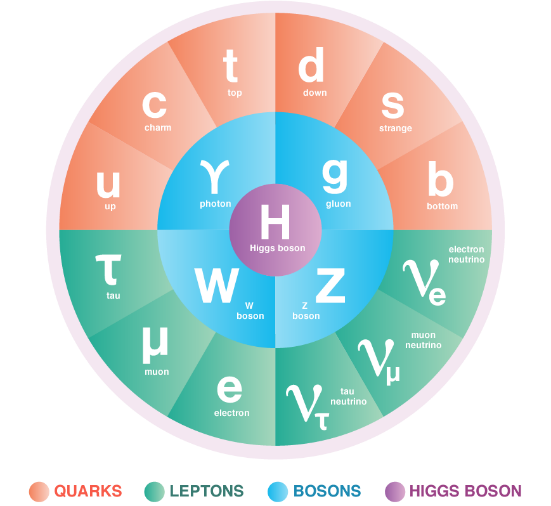
\includegraphics[width=0.7\columnwidth]{Chapter1/images/particles.png}
\caption{Fermions and bosons of the Standard Model~\cite{standard_model}.}
\label{fig_standard}
\end{figure}

\newpage

The Strong Force theoretical foundation, Quantum Chromodynamics (QCD), is a well-established theory describing the interaction between quarks through the exchange of gluons. 

Yet, key phenomena in strong interactions, like the confinement of quarks and gluons into hadrons\footnote{Hadrons are composed of quarks, and therefore they experience the strong nuclear force.} and the creation of mass, have remained unclear.

In extreme environments such as high-temperature T, or the high baryon density $\rho$, the confined baryonic matter forms a new state of matter called the quark-gluon plasma (\gls{QGP})~\cite{phase_diagram}. Hot deconfined matter dominated the early cosmos just a few microseconds after the Big Bang, but compact stars may also contain cold and baryon\footnote{Baryons are composed of three quarks, and they make up most of the visible matter in the universe.}-rich quark matter in their interiors.

A well-established non-perturbative approach to solving quantum chromodynamics theory is known as Lattice \gls{QCD}. LQCD can also be used to address issues like the confinement mechanism and chiral symmetry breaking, the role of topology, and the equilibrium properties of \gls{QCD} at finite temperature~\cite{lattice_qcd}. 

\section{Studies of nuclear matter and its forms}
 The strong interacting matter phase diagram represents various phases, such as liquid, gas, or plasma. It also describes the borders between these states and types of transitions (see Figure~\ref{fig_phase}). The diagram illustrates the experimental results and theoretical predictions for the properties of strongly interacting matter.

The direct insight into the \gls{QGP} is impossible, as it rapidly changes to the hadronic gas in a heavy-ion reaction. The experimental search for \gls{QGP} in heavy-ion collisions was related to several model predictions of possible \gls{QGP} signatures: 
\begin{itemize}
    \item suppressed production of charmonium states (bound states of a charmed quark and a charmed antiquark), in particular, $\mathrm{J/\psi}$ mesons \cite{MATSUI1986416},
    \item enhanced production of strange and multi-strange hadrons from the \gls{QGP} \cite{strageness},
    \item characteristic radiation of photons and dilepton pairs from the \gls{QGP},
    \item elliptic flow \cite{Stefaniak:2022dxo},
    \item inelastic fluctuations \cite{Stefaniak:2022dxo}.
\end{itemize}
The results of the QGP search program at The Super Proton Synchrotron \gls{SPS} on central collisions of medium and heavy nuclei were found to be adequate with the QGP predictions~\cite{Rafelski_2015}.

The crossover transition region was experimentally investigated at the Large Hadron Collider (\gls{LHC}) and Relativistic Heavy Ioc Colllider (\gls{RHIC}). This region is characterized by a low baryon chemical potential and high temperatures (around $150\,\mathrm{MeV}$), at which the number of baryons to antibaryons is equal. Lattice \gls{QCD} calculations show that the transition at $\mu_{B} = 0$ is a crossover transition~\cite{Aoki_2006}. The nuclear matter is expected to hadronize at the temperature of 155--160 MeV~\cite{Bazavov_2012, Stachel_2014}.



\begin{figure}[!h]
\centering
 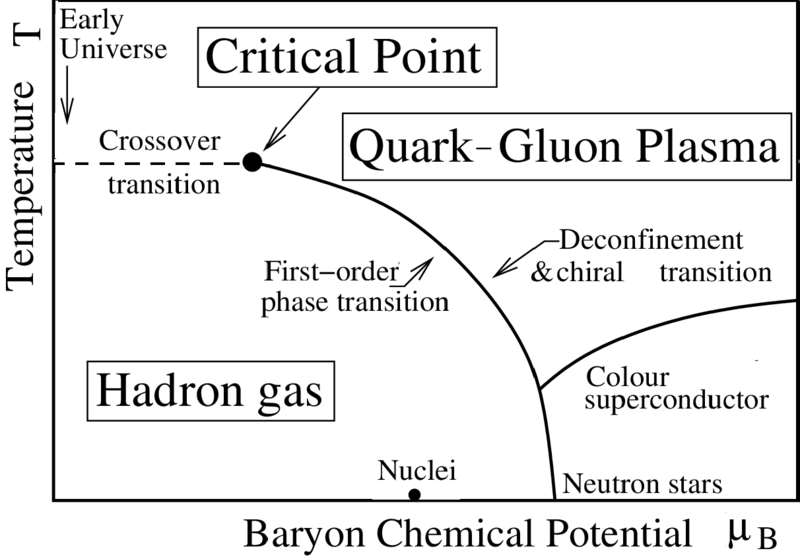
\includegraphics[width=0.65\columnwidth]{Chapter1/images/phase.png}
\caption{The phase diagram illustrating the regimes of confined and deconfined states of nuclear matter. The critical point separates the region of a cross-over (explored by \gls{RHIC} and \gls{LHC}) from that of a first-order phase transition to be studied by the CBM experiment~\cite{friese_diagram}.}
\label{fig_phase}
\end{figure}
Figure \ref{fig_phase} also depicts structures at higher baryon-chemical potentials, such as a chiral and a deconfinement first-order phase transition merging at a critical point. To date, none of these structures or phases have been discovered. As previously stated, first-principles theories, such as perturbative QCD, continue to struggle to generate solid predictions for matter characteristics at higher baryon-chemical potentials~\cite{Sakai_2008, Fischer_01, Tawfik_01}. 


%\section{Physics goa}

\section{Probing dense nuclear matter with heavy-ion collisions}

Heavy-ion collisions at beam energies between \agev{2} and \agev{11} have an enormous potential to explore many aspects of the phase diagram. Figure \ref{fig:cbm_density} represents the time evolution of Au+Au collision system at \agev{10} beam energy. Similar densities as those produced in heavy-ion collisions are expected to prevail during the supernovae core collapse and in the core of neutron stars. Furthermore, the calculations of different transport models and hydrodynamics show that the density of the fireball will reach more than $8\rho_{0}$ during the Au+Au collisions at \agev{10}~\cite{CBM_physics}.

\begin{figure}[!h]
    \centering
    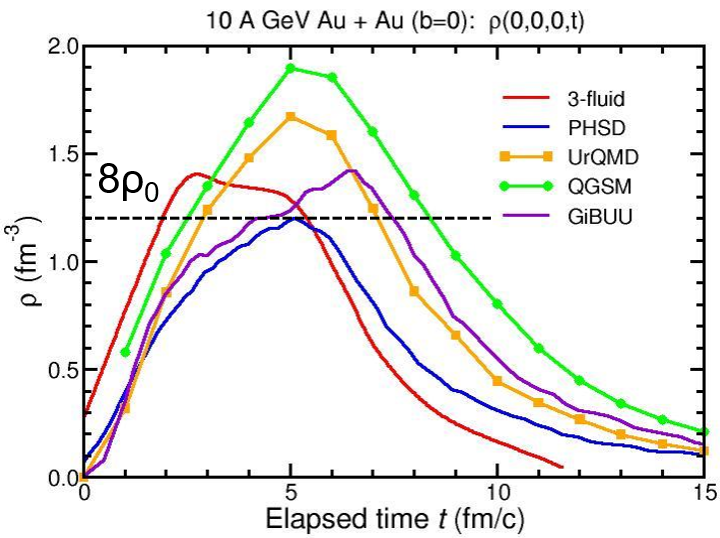
\includegraphics[width=0.65\columnwidth]{Chapter1/images/CBM_density.png}
    \caption{The time evolution of the central net-baryon density $\rho(t)$ calculated using different transport models and 3-fluid hydrodynamics of a head-on Au+Au collision at \agev{10} energy~\cite{CBM_physics}.}
    \label{fig:cbm_density}
\end{figure}

Figure~\ref{fig_heavyion} depicts the presumed evolution of the heavy-ions collision. Depending on the temperature and net-baryon density of the system, there are two outcomes described in Figure~\ref{fig_heavyion}. It illustrates the various forms of QCD matter intervening during the subsequent phases of the hadronic and heavy-ion collisions.

\begin{figure}[!h]
\centering
 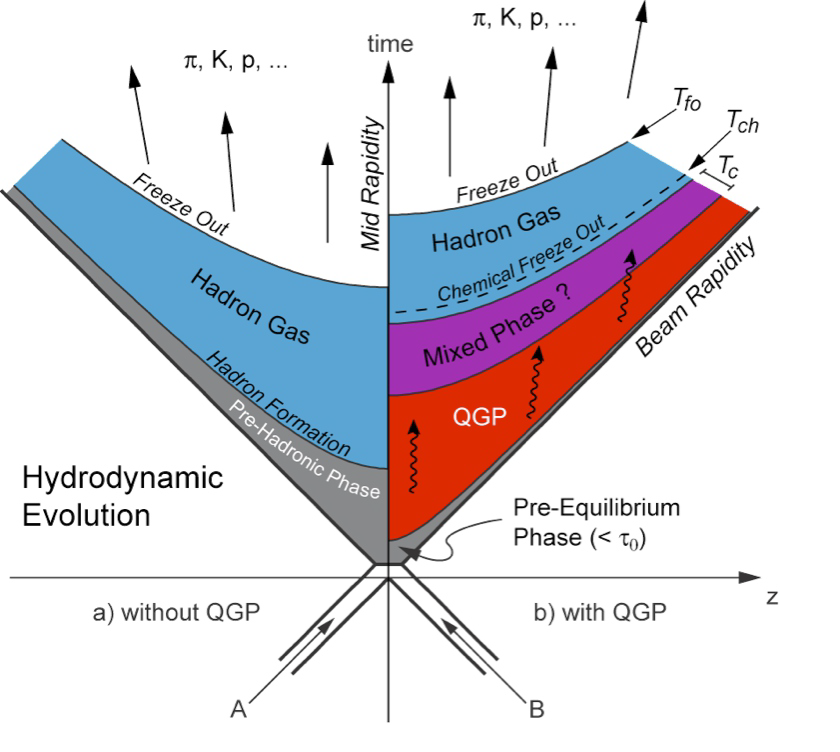
\includegraphics[width=0.55\columnwidth]{Chapter1/images/heavyion.png}
\caption{Schematic representation of the various stages of a HIC as a function of time t and the longitudinal coordinate z (the collision axis). The critical temperature is represented by $T_c$, whilst the freeze-out and chemical freeze-out temperatures are indicated by $T_{fo}$ and $T_{ch}$, respectively~\cite{Sahoo:2745520}.}
\label{fig_heavyion}
\end{figure}
\newpage
 After the collision (right side of the graph in Figure~\ref{fig_heavyion}), the system enters a pre-equilibrium phase, followed by a deconfined QGP medium and a probable mixed phase (which should exhibit first-order phase transition signals).

Heavy-ion experiments around the world have been exploring the facets of the phase diagram through systems characterized by a wide range of temperatures and densities. Figure~\ref{fig:cbm_rates} shows the interaction rates of existing and planned heavy-ion experiments. In the upcoming facilities, the main focus is put on the highest possible luminosity. Groundbreaking heavy-ion experiments at AGS in Brookhaven and at low CERN-SPS beam energies have investigated the QCD phase diagram at high baryo-chemical potentials. Because of the detector technologies available at the time, these observations were limited to abundantly generated hadrons and di-electrons with severely constrained statistics.

\begin{figure}[!h]
    \centering
    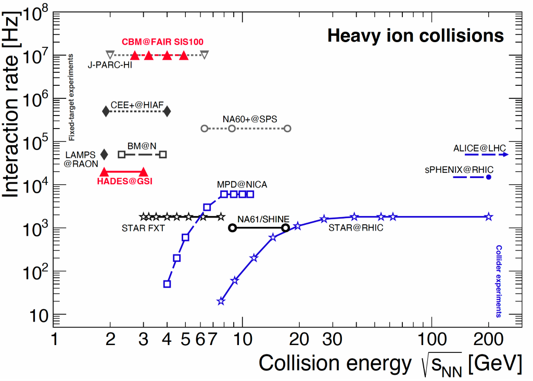
\includegraphics[width=0.7\columnwidth]{Chapter1/images/interaction_rates.png}
    \caption{Interaction rates achieved by existing and planned heavy-ion experiments as a function of the center-of-mass energy. “STAR FXT” denotes the fixed-target operation of STAR.  Blue symbols show collider experiments, whereas black and gray symbols show fixed-target experiments~\cite{Ablyazimov_2017}.}
    \label{fig:cbm_rates}
\end{figure}

The NA61/SHINE experiment at CERN-SPS has been searching for the first-order phase transition by investigating collisions of hadrons with light and heavy-ion beams (pions, protons, beryllium, argon, and xenon ions) with a variety of nuclear targets~\cite{CBM_physics, Turko:2301677}. The collision energies varied from \agev{13} to \agev{158} depending on the size of the colliding system~\cite{na61energy}. 

The Solenoidal Tracker at \gls{RHIC} has
performed a beam energy scan $\sqrt{s_{NN}} =$~\gev{7.7}--\gev{200}, where $\sqrt{s_{NN}}$ is the center of mass energy of the nucleus-nucleus (NN) system. The studied systems included gold, uranium, aluminum, deuteron, helium, and zirconium ions and protons ($\sqrt{s_{NN}}=$~\gev{200})~\cite{Stefaniak:2022dxo}. The Beam Energy Scan (\gls{BES}) phase I program findings shed light on first-order phase transition in the QCD phase diagram and the turn-off of the quark-gluon plasma distinctive fingerprints at low collision energy. BES phase II program (BES II) covers the $\sqrt{s_{NN}}$ from \agev{7.7} to \agev{19.6} in the collider mode and from \agev{3} to \agev{7.7} in the fixed-target mode~\cite{STAR2, STAR1}.
The studies conducted at \gls{STAR} and A Large Ion Collider Experiment (\gls{ALICE}) at \gls{LHC} aimed at studies related to the \gls{QGP} and revealed that the partonic degrees of freedom prevail at the early phase of the fireball evolution~\cite{CBM_physics}.


The Nuclotron at the Joint Institute for Nuclear Research (JINR) in Dubna is preparing the fixed-target experiment BM@N to explore heavy-ion collisions at gold beam energy up to roughly \agev{4}. Furthermore, the Nuclotron-based Ion Collider fAcility NICA with the Multi-Purpose Detector (MPD) is being built at JINR. The NICA collider is intended to operate at collision energies ranging from $\sqrt{s_{NN}} =$~\agev{8} to \agev{11}, with reaction rates up to \khz{6} for minimal bias Au+Au collisions~\cite{Ablyazimov_2017}.

The High-Acceptance DiElectron Spectrometer (\gls{HADES}) detector at SIS18 detects hadrons and electron pairs in heavy-ion collision systems at reaction rates of up to \khz{20} and beam energy of 1-\agev{2}~\cite{Ablyazimov_2017}.


Unfortunately, due to luminosity or detector limits, the investigations with the previously mentioned experiments were unable to measure rare observables with extremely low production cross-sections and must instead focus on abundantly generated particles. As the \gls{CBM} experiment will measure with event rate up to $10\,\mathrm{MHz}$, it is well-positioned to explore many facets of the \gls{QCD} matter. \gls{CBM} is a fixed target experiment that aims to measure rare particles as probes of dense matter with very good precision at beam energies up to \agev{11} or $\sqrt{s_{NN}}$ = \gev{4.9} (up to \agev{14} for light nuclei and \agev{29} for protons) and interaction intensities up to $10\,\mathrm{MHz}$~\cite{cbmus}.

The \gls{CBM} experiment will be able to explore the equation of state at densities (2–6 times saturation density) close to those existing in cores of massive neutron stars, supernovas, and neutron star mergers (4-5\,$\rho_{0})$~\cite{Senger_2020}. The majority of the experimental observables which are sensitive to the properties of dense nuclear matter, like the flow of (anti-) particles, higher moments of event-by-event multiplicity distributions of conserved quantities, multi-strange (anti-) hyperons, di-leptons, and particles containing charm quarks are prone to the statistics. Therefore, the key feature of successful experiments is high rate capability, which ensures high precision~\cite{Ablyazimov_2017}. 

The \gls{CBM} experiment aims to investigate:
\begin{enumerate}
    \item the equation of state of baryonic matter at neutron star densities,
    \begin{itemize}
        \item differential collective behavior of protons, pions, and deuterons - the collective hadrons motion provides information on the dense stage of the heavy-ion collision. It is driven by the pressure gradient created at the beginning of the fireball evolution~\cite{Reisdorf_2007}.
        \item hyperons and their interactions - are preferentially produced in the dense phase of the fireball via sequential collisions~\cite{CBM_physics}.
    \end{itemize}
    \item modifications of hadron properties in the dense baryonic matter and the onset of chiral symmetry restoration. These phenomenons affect the invariant-mass spectra of di-leptons, which will be measured both in the electron and the muon channel,
    \item phase transitions from hadronic matter to quarkonic or partonic matter:
    \begin{itemize}
        \item the excitation function of multi-strange hyperons, which are driven into equilibrium at the phase boundary~\cite{CBM_physics},
        \item the excitation function of the invariant mass spectra of lepton pairs which reflect the fireball temperature, and, hence, may reveal a caloric curve and a first-order phase transition~\cite{CBM_physics},
        \item the excitation function of higher-order event-by-event fluctuations of conserved quantities such as strangeness, charge, and baryon number, which are expected to occur in the vicinity of the critical point~\cite{CBM_physics}.
    \end{itemize}
    \item hypernuclei (double $\Lambda$, strange di-baryons, etc.) and the measurement of their lifetime, which will provide information on the hyperon-nucleon and hyperon-hyperon interaction~\cite{CBM_physics},
    \item charm production mechanisms~\cite{CBM_physics}.
\end{enumerate}
A detailed description and explanation of the \gls{CBM} physics program can be found in the \gls{CBM} Physics Book~\cite{CBM_physics} and in~\cite{Ablyazimov_2017}.




\section{Overview of the FAIR facility}
The Facility of Antiproton and Ion Research in Europe (\gls{FAIR})~\cite{fair} is a future international research facility for accelerator-based research. 

\begin{figure}[!h]
    \centering
    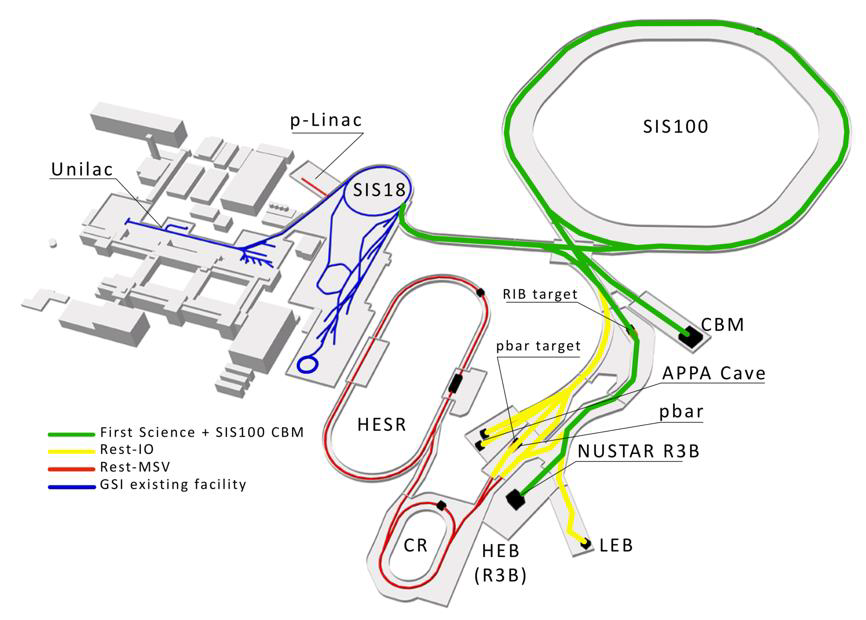
\includegraphics[width=0.85\columnwidth]{Chapter1/images/fair2.png}
    \caption{Overview of the GSI/FAIR research facility~\cite{fair}. The existing beam lines of the \gls{GSI} facility are denoted with blue lines. The planned facility and the corresponding experiments are located to the right.}
    \label{fig:fair}
\end{figure}

It will provide unique research opportunities in hadron and nuclear physics, atomic physics, nuclear astrophysics, materials research, plasma physics, and radiation biophysics, including developing novel medical treatments and applications for space science~\cite{fair1}. 
 
FAIR (see Figure \ref{fig:fair}) will extend GSI with Schwerionensynchrotron 100 (SIS100) accelerator, storage rings, and dedicated experiments from different fields, namely Atomic Physics, Plasma physics and Applications (APPA), antiProton ANnihilation at DArmstadt (PANDA), Nuclear Structure, Astrophysics, and Reactions (NUSTAR), and Compressed Baryonic Matter (\gls{CBM}). The latest status of SIS100 and its plans were recently described by Spiller~\cite{Spiller_2020}.

The SIS100, which will provide high-intensity beams of protons up
to energy of \gev{29}  with intensities up to $2.5\times 10^{13}$~protons/cycle and nuclei up to \agev{15} for $Z/A = 0.5$. Gold or uranium beams with kinetic energies up to \agev{11} will be available. Typical intensities for the heavy ions also depend on charge state and vary from $2.7\,\mathrm{GeV/u}$ for $\mathrm{U^{28+}}$ ions with $5\times 10^{11}$\,ions/cycle to $10\,\mathrm{GeV/u}$ for $\mathrm{U^{92+}}$ ions with $4\times 10^{10}$\,ions/cycle. High-intensity secondary beams will be produced by a large acceptance Superconducting Fragment Separator, which investigates very efficiently rare isotopes created in reactions with the primary beams. 

Moreover, a secondary antiproton beam will be produced by bombarding a metal target with $27.5\,\mathrm{GeV}$ protons. The collection of the pbar will be achieved with the \footnote{Magnetic horn is a high-current, pulsed focusing device used for the antiproton beam.}{magnetic horn}. The separation of the antiprotons from primary protons
and other secondary particles will be provided by the succeeding pbar separator, which will transfer antiprotons to the collector ring (CR)~\cite{SI100_CR}.




\section{Compressed Baryonic Matter experiment, subdetectors and their tasks}
The Compressed Baryonic Matter (\gls{CBM}) experiment is currently being constructed at \gls{FAIR}. Figure~\ref{fig:exp} depicts the CAD drawing of the \gls{CBM} experiment. The beam enters the experimental cave from the left side and traverses the High Acceptance Di-Electron Spectrometer (\gls{HADES}) experiment to finally reach the target of the \gls{CBM} experiment. 

\begin{figure}[!h]
    \centering
    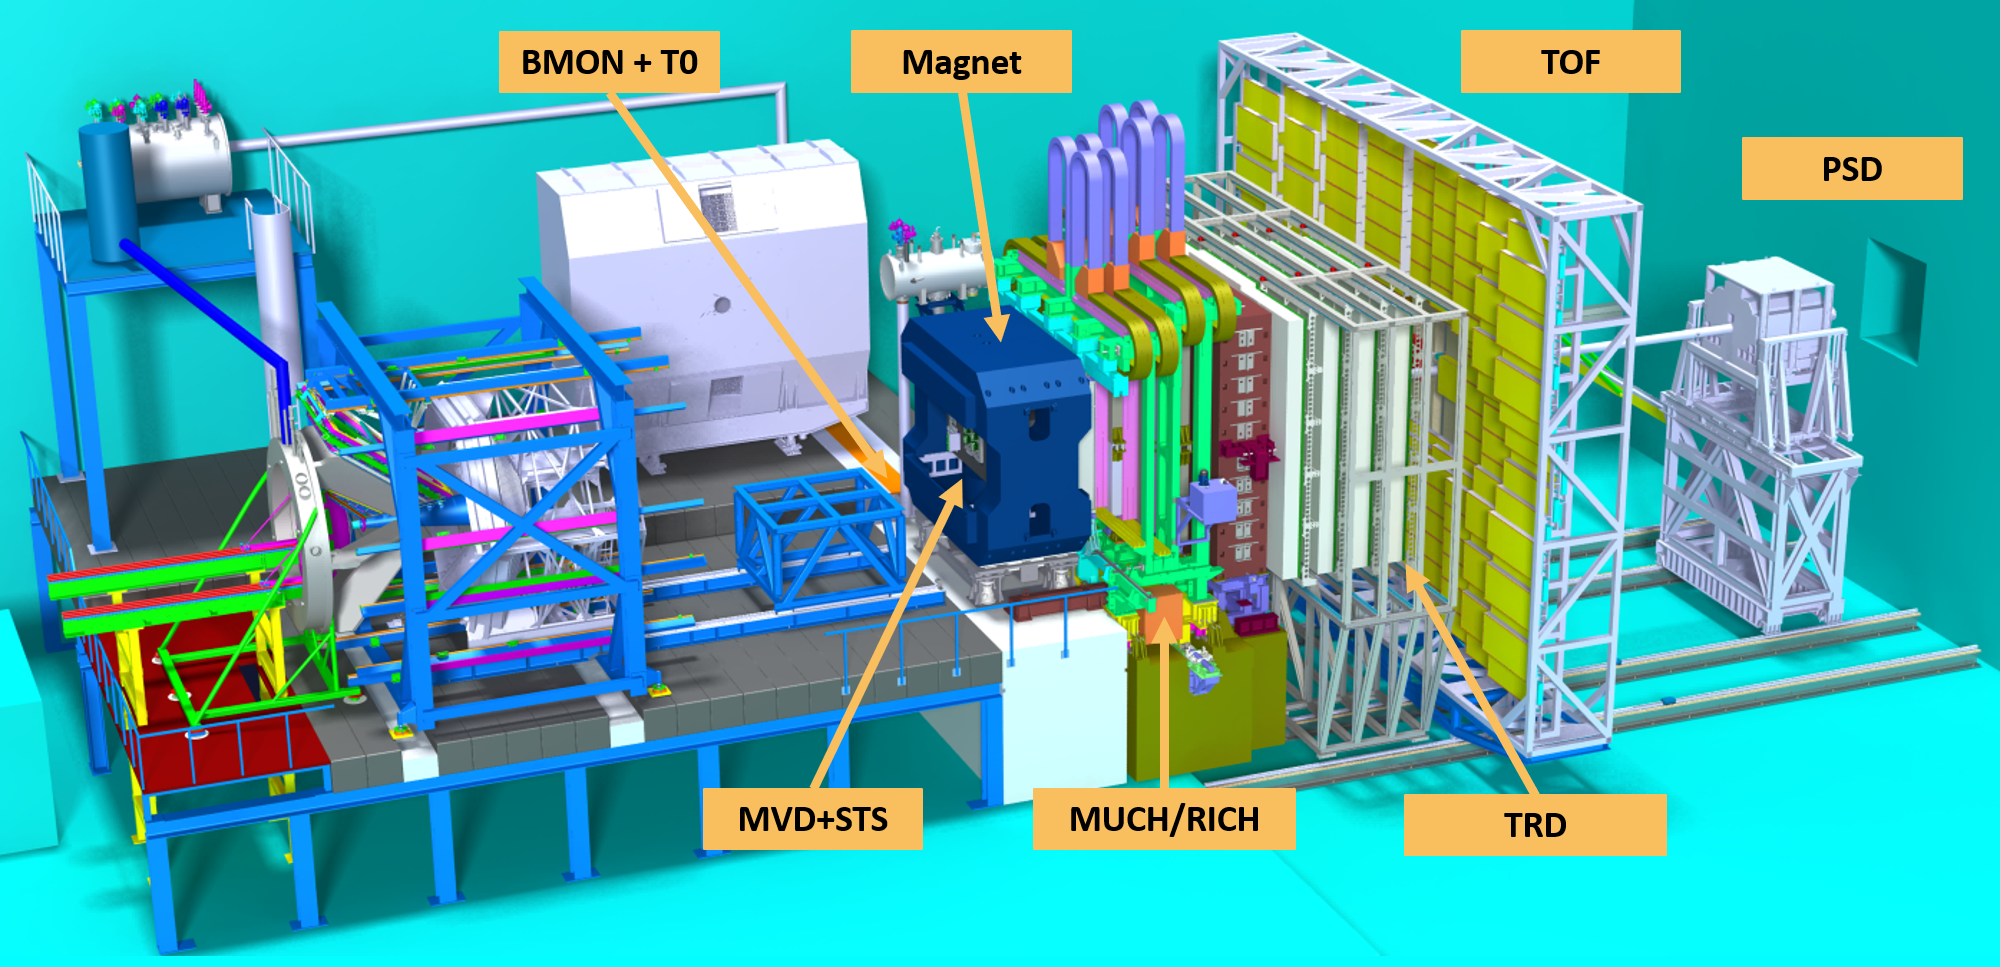
\includegraphics[width=1\columnwidth]{Chapter1/images/CBMnew.png}
    \caption{HADES experiment on the left side and the \gls{CBM} experiment on the right side.}
    \label{fig:exp}
\end{figure}

The main features of the experiment are described below:
\begin{itemize}
\item tracking acceptance: $\SI{2.5}{\degree} < \theta_{lab} < \SI{25}{\degree}$,
\item peak event intensities up to 10 MHz for Au+Au systems,
\item fast and radiation hard detectors,
\item free-streaming triggerless Data Acquisition (\gls{DAQ}),
\item 4D tracking (spatial and time),
\item online event reconstruction and selection,
\item data rates from the readout electronics of up to 2~TB/s.
\end{itemize}


In order to get valuable insight into the physics observables proper detector systems need to be developed. The detector concept is based on identifying the stable charged particles that are often decay products of resonances and unstable particles. Charged particles can be bent in a magnetic field of known strength to investigate their momentum. Together with information from Time-of-flight (\gls{TOF}) the mass of particles can be distinguished. Di-leptons are considered special due to their nature. They may contain undisturbed information from the early, dense phase of the fireball evolution. On the other hand, it is necessary to separate them from the abundant pions. In order to perform the complete analysis, the following detector systems are foreseen for the \gls{CBM} experiment:\bigbreak


\textbf{Beam monitor, or T0 (\gls{BMON})} and its conceptual design, was summarized during the 40th \gls{CBM} Collaboration Meeting~\cite{bmon}. Two separate stations in front of the target are made out of high-purity poly-crystalline CVD diamond material. This detector is foreseen to monitor beam quality (position, time structure) and determine the start time of the reaction.\bigbreak

\textbf{Micro Vertex Detector} (\gls{MVD}) consists of four planar stations with Monolithic Active Pixel Sensor (\gls{MAPS}) chips. A station layout and distance from the target can be tailored to the needs of a specific run, for example, to optimize vertexing or tracking. The vertexing detector geometry aims at a precision of secondary vertices determination of about 50 -- \mum{100} along the beam axis. The main aim is decay vertex identification of the very short-lived particles such as charmed mesons, which decay within a few hundred \SI{}{\micro\metre} behind the target, as well as background rejection in di-electron spectroscopy~\cite{MVD}.\bigbreak

 \textbf{Silicon Tracking System} (\gls{STS}) which is responsible for tracking charged particles inside the magnetic field. The \gls{STS} is located inside a superconducting dipole magnet~\cite{Malakhov:109025}. The charged particles traversing the active volume of \gls{STS} are bent due to the applied magnetic field. The trajectories of charged particles inside the magnetic field will be determined by MVD and STS across a \SI{1}{\metre} length downstream of the target~\cite{Heuser:54798}.\bigbreak
 
\textbf{Muon Chamber System} (\gls{MUCH}) is the fourth subsystem of the \gls{CBM} experiment. It is dedicated to muon detection (for example rare particles decaying into muons like $J/\psi$) and track reconstruction. This concept is based on the layered design of the hadron absorbers (5 layers), separated with tracking detector planes which are based on Gas Electron Multiplication (\gls{GEM}) and Resistive Plate Chambers (\gls{RPC}) detectors~\cite{MUCH}.\bigbreak

\textbf{Ring Imaging Cherenkov Detector} (\gls{RICH}) is responsible for electron identification via Cherenkov radiation~\cite{RICH}. The detector consists of \SI{1.7}{\metre} a long $\mathrm{CO_{2}}$ gas radiator with pion threshold for Cherenkov radiation of \agevc{4.65}, two arrays of mirrors, and photon detector planes. It allows separating electrons from pions up to \agevc{8}. The models predict that a pion suppression on the level of 500 will be accomplished thanks to the high granularity (about 55 000 channels) and high number of photons per ring~\cite{RICH}.\bigbreak

\textbf{Transition Radiation Detector} (\gls{TRD}) suppresses pions and  supports track reconstruction with 9-10 detector layers grouped into 3 stations. It is placed between \SI{4}{\metre} to \SI{9}{\metre} downstream of the target, and the total active area reaches \SI{600}{\square\metre}. Because the RICH electron identification capabilities are limited to the lower momentum range ($p < $~\agevc{5}), the TRD will be employed as a supplementary device to supplement and expand the electron identification into higher momenta. The TRD configuration designed for the SIS100 CBM setup will therefore be capable of identifying electrons beyond a momentum threshold of $p > $~\agevc{1} with a 90\% efficiency while reducing the hadronic background by a factor of 10 - 20. The working principle of the detector is based on the phenomenon that the ultra-relativistic particles traversing through a medium with alternating dielectric constant produce transition radiation. It is composed of two parts, the readout chamber, and the radiator. The photons are generated by the electrons passing through the radiator, while the heavier pions do not produce any radiation. For detection of the produced radiation, multi-wire proportional chambers will be used with a $\mathrm{85\% Xe/15\% CO_{2}}$ gas mixture)~\cite{TRD}. \bigbreak

\textbf{Time-of-Flight Detector} (\gls{TOF}) is designed to identify hadrons (pions, kaons, and protons). As the name indicates, the detector measures the time-of-flight of the reaction products with Multi-Gap Resistive-Plate Chambers (\gls{MRPC}). The \glspl{MRPC} have an excellent time resolution of \SI{60}{\pico\second}.  It might be located between \SI{6}{\metre} and \SI{10}{\metre} (depending on the physics objectives) and will cover an area of about \SI{120}{\square\metre}~\cite{TOF}. \bigbreak

\textbf{Projectile Spectator Detector} (gls{PSD}) is the last subsystem of the \gls{CBM} experiment, and it determines the collision centrality and event plane. The detector is meant to measure the nucleons from a projectile nucleus in heavy-ion collisions. The proposed 44 module design of the PSD covers a large transverse area around the beam spot position, such that most of the projectile spectator fragments deposit their energy in the \gls{PSD}. The detector concept is a compensating hadron calorimeter consisting of lead-scintillator sandwich modules~\cite{PSD}.\bigbreak


The CBM detector system can be used in two operation modes: the first one is optimized for electron identification (electron configuration) and the second is designed for muon identification (muon configuration). In the first one, all the subsystems apart from MUCH will be involved. In the muon configuration, the \gls{RICH} detector is replaced by \gls{MUCH}.

For the high-rate CBM experiment, the triggerless data read-out and acquisition system plays a crucial role. The time-stamped signals will be read out without event correlation and transferred to a high-performance computing farm, the GSI GreenIT Cube. The online event reconstruction and selection will be performed by high-speed algorithms. In the first step, the tracks of the charged particles are reconstructed from the space and time information from the various detector signals. This process is based on the Cellular Automaton (\gls{CA}) track finder~\cite{CA}. Subsequently, the particles are identified, taking into account secondary decay vertices and information from \gls{RICH} or \gls{MUCH}, \gls{TRD}, and \gls{TOF}. Finally, the particles are grouped into events, which will be selected for storage if they contain important observables. In parallel, the event and its plane are characterized using information from the PSD.

Another important online system is called Experiment Control System (\gls{ECS}). It is a software structure that aims to provide automatization, monitoring, and control of hardware and the detector subsystems. A detailed description of \gls{ECS} and the detector-specific control system (\gls{DCS}) will be given in Chapter~\ref{chap:online_systems}.



\section{Thesis overview and its rationale}
The thesis consists of seven chapters. The second chapter introduces the role of silicon trackers in large scientific experiments and discusses the design details of \gls{STS}, including the physics performance and experimental challenges. Those elements define the requirements for the Detector Control System (\gls{DCS}). The third chapter serves as an introduction to the control and monitoring of a large experiment, with an extended focus on the detector-related slow control system and the developed control framework. The following three chapters are focused on the results and their consequences for the experiment:
\begin{itemize}
    \item chapter 4 covers the first implementations of the mentioned control framework. The first application is related to the slow control interface for the Front-End Electronics (\gls{FEE}) readout. The second and third examples are related to the irradiation studies of the powering modules for the Low Voltage (\gls{LV}) powering of \gls{STS} electronics and thermal cycling of Front-end boards (\glspl{FEB}). The performed studies and results of these activities are discussed in detail,
    \item chapter 5 describes the efforts to design and test a distributed sensing system for \gls{STS} with a focus on humidity sensing. Three considered technologies feature capacitive sensors, fiber optic sensors, and remote sensing with the use of a sampling system. The chapter focuses on the design choices and characterization of the fiber Bragg grating-based sensors. 
    \item chapter 6 focuses on controlling a small-scale prototype version of \gls{STS} in the \gls{mCBM} experiment. The first sections describe in detail the hardware and software solutions implemented in the detector. Subsequently, the results from the full-blown \gls{DCS} are presented and discussed, including the radiation effects on the silicon sensors and general considerations about the power dissipation of different elements of \gls{STS} powering scheme. Moreover, considerations about the \gls{DCS} are given. 
\end{itemize}
The last part of the thesis summarizes the results and sheds light on the next steps toward the realization of \gls{STS} and its controls. The most important findings and results from the performed studies are also discussed.
\chapter{The STS and its role in the CBM experiment}
\label{chap:CBM_STS}

%\section{Overview of the Silicon Tracking System (STS)}
All semiconductor based detector systems include very similar functions. The signals from the detector channels have to be amplified and processed for storage and analysis. The silicon sensors, analog-digital converter and all the necessary support structures are often referred to as a detector module. Nevertheless, there are many parameters that have to be optimized in order to achieve the detector performance.

The use of microstrip silicon sensors was demonstrated in other experiments around the world. It's design and thickness are primarily dependent on the constraints related to the scaterring and signal over noise ratio. 

This chapter aims to present an introduction to the silicon based detector systems and general working principles. Subsequently, the design of the \gls{STS} is discussed with focus on the hardware and its control. At last, the requirements for the detector control system are considered. 

\subsection{Role of the semiconductors based detector}

Semiconductors can be considered as ionization chambers, which are features a pair of electrodes and applied external voltage. The particles passing through the volume of a sensor may result in forming an electron and hole pair. A typical charge deposition by a minimum ionizing particle in a \SI{300}{\micro\metre} thick wafer is around 25000 electron-hole pairs. The deposited charge is retrieved by one or more strips per side, what results in position determination. The analog signals are converted into digital ones, processed and analyzed.

In the simplest case, a plate could be used as an electrode, but it wouldn't be possible to determine the position of a particle very precisely. To address this problem, the electrodes can be segmented into strips. Figure~\ref{fig_si} shows an example of implementing segmented electrodes to determine the particle position. In order to achieve the two-dimensional information, the second electrode has usually an inclination of a few degrees. Apart from microstrip sensors, there are also for example pixel devices which enable determining two-dimensional positions. It can be achieved either by proper segmentation of the electronics or designing the geometry.  

\begin{figure}[!h]
\centering
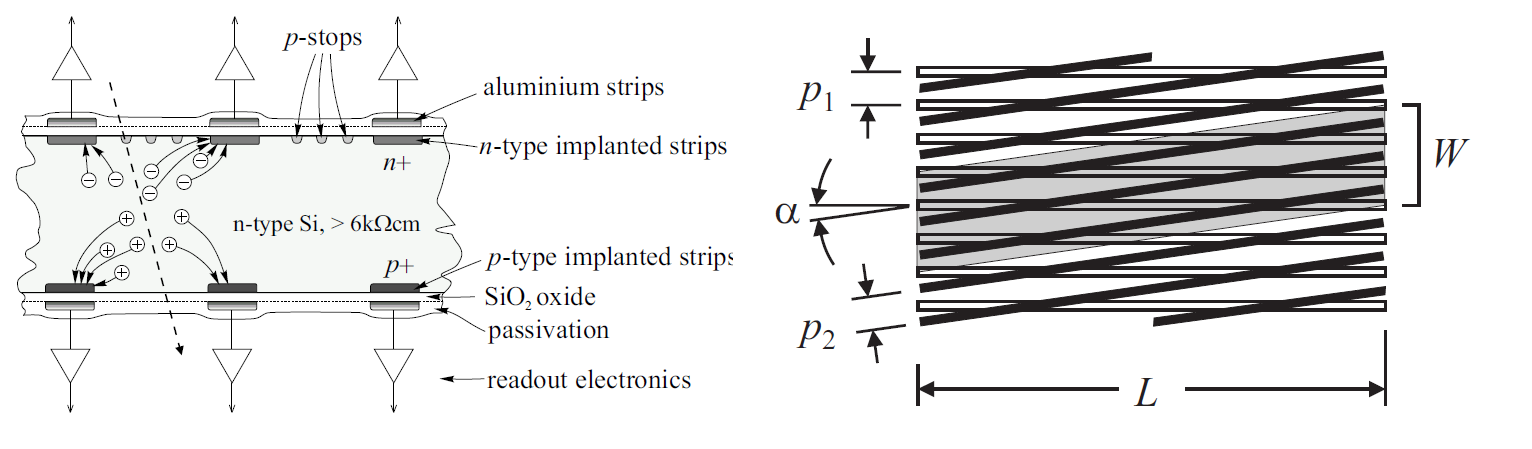
\includegraphics[width=1\columnwidth]{Chapter2/images/silicons.png}
\caption{The segmented electrode enables defining the particle position (left)~\cite{Sokolov:2006vdx}. The right scheme depicts the strips oriented at a small angle, which aims to reduce fake hits~\cite{Spieler}.}
\label{fig_si}
\end{figure}
\newpage


The sensitive volume of a silicon sensor produces the average signal current given by 
\begin{equation}
    Q_{s} = \frac{E}{E_{i}}e
\end{equation}
where E is the absorbed energy, $E_{i}$ is the energy required to form a charge pair. The energy needs to be greater than the bandgap, so that the electron can move to the conduction band. The silicon has a gap of 1.12~eV. Nevertheless, the commonly used ionization energy for silicon is about 3.6~eV. This effect is related to the fact that only about 30\% of the particle's energy is converted into electrical signal, the rest goes into phonon excitation.



\section{Radiation damage to the silicon sensors} 

The most important formula which allows for the trackers to be used in particle physics is Bethe-Bloch formula:

\begin{equation}
-\dfrac{\mathrm dE}{\mathrm dx} = 4 \pi N_{a} r_{e}^{2} m_{e} c^{2} z^{2}  \dfrac{Z}{A} \frac{1}{\beta^{2}} \left[ \frac{1}{2}\ln(\frac{2m_{e}\gamma^{2}c^{2} T_{max}}{I^{2}}) - \beta^{2} -  2\frac{\delta(\gamma)}{Z}\right]
\end{equation}

Where z is the charge of the particle, $T_{max}$ is the maximum kinetic energy that can be imparted to a free electron in a single collision, I is the mean excitation energy, Z the atomic number, A the atomic mass, $N_{A}$ the Avogadro’s number, $m_{e}$ the electron mass, c the speed of light, $r_{e}$ the classical electron radius, $\beta = v/c$ and $\gamma = \frac{1}{\sqrt{1-\square\beta}}$ and $\delta$ density effect correction. It describes the average energy loss of a charged particle in a given medium (for example, gas or a semiconductor). 

Radiation damage can be divided into two main groups: displacement damage and ionization damage. The first mentioned phenomenon is related to the incident particles displacing the silicon atoms from their position in the lattice. The ionization damage occurs in the insulating layers of the sensor. 

The influence of the radiation on the silicon is described by so-called Hamburg model. 

The traversing particles are not only causing the ionization of the lattice, but also interact with the silicon via electromagnetic and strong forces. Atoms can be displaced and create defects. Those defects populate new levels in the band gap, changing the properties of the silicon. That’s why the performance of the silicon sensor will degrade over time, what should also be considered while designing an experiment. The leakage current of a sensor after irradiation is related to the fluence as follows:
\begin{equation}
\label{eq:fluence}
    I_{d} = I_{0} + \alpha + \phi + Ad
\end{equation}
where $I_{0}$ is the leakage current before the irradiation, $\alpha$ is a damage coefficient dependent on particle type and temperature, $\phi$ is the particle fluence, d is the detector thickness, and A is the area. 
Typical values for the damage coefficeint reach 


\begin{equation}
\label{Sil:temp}
    I_{R}(T) \propto T^{2}e^{\frac{-E}{2kT}}
\end{equation}
 By assuming that one of the  temperature sensors at a similar height as the silicon sensors mimics their temperature. This assumption clearly doesn't consider several effects like silicon sensors' self-heating. Nevertheless, it allows us to scale down leakage current to $20\,^{\circ}$C using the equation \ref{Sil:scal}.
 
\begin{equation}
\label{Sil:scal}
    \frac{I_{R}(T_{2})}{I_{R}(T_{1})} = (\frac{T_{2}}{T_{1}})^{2}e^{\frac{-E}{2kT}\frac{T_{1}-T_{2}}{T_{1}T_{2}}}
\end{equation}

\begin{figure}[!h]
\centering
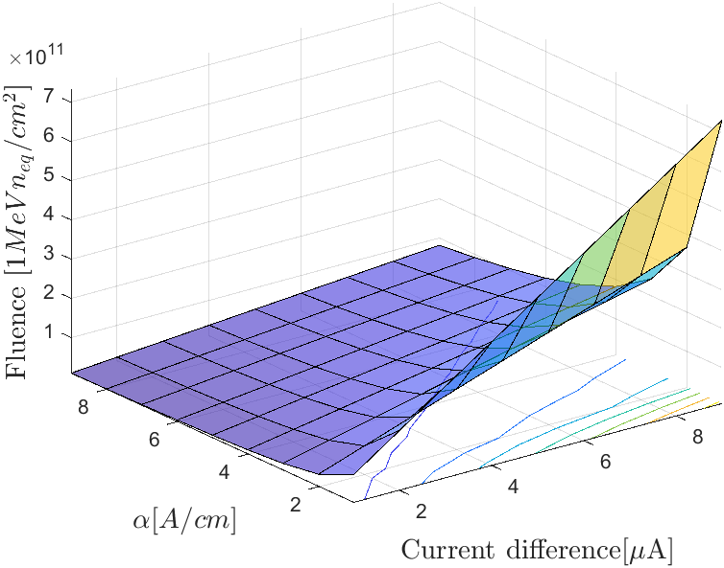
\includegraphics[width=0.65\columnwidth]{Chapter2/images/Leakage_current.png}
\caption{Fluence estimations based on the equation~\ref{eq:fluence} for the typical leakage changes during the \gls{mCBM} experiment.}
\label{fig_leakage}
\end{figure}

\begin{figure}[!h]
\centering
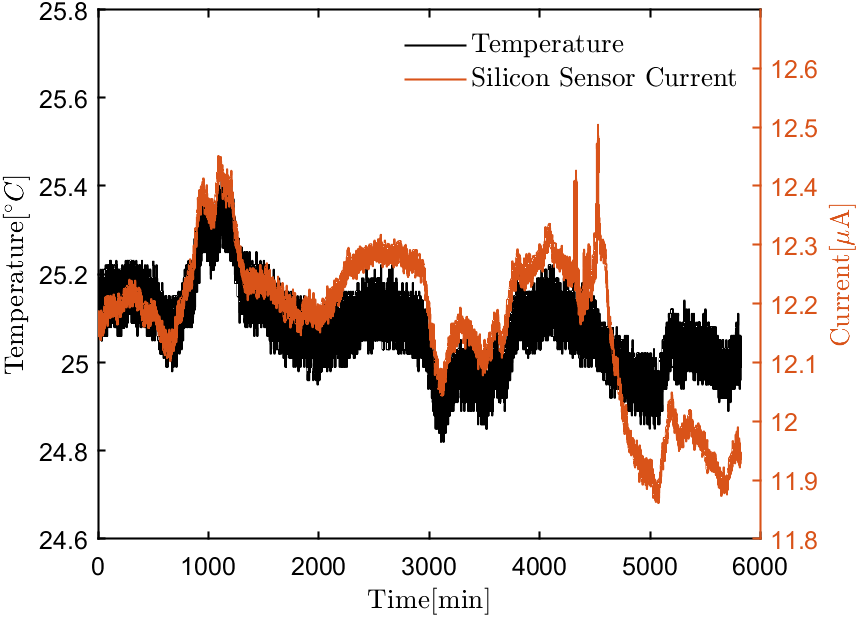
\includegraphics[width=0.65\columnwidth]{Chapter2/images/currenttempnobeam.png}
\caption{The first proposition of the CBM readout chain based on separate DPB and FLIB boards \cite{CRI}}
\label{fig_leakage1}
\end{figure}




\section{Design of STS}


The physics observables together with the foreseen accelerator specifications mentioned in the previous chapter define the requirements for the detector system. The \gls{STS} is designed to provide track reconstruction and momentum determination of the charged particles. The detector has to work with ion beam energies from 2 to 14 AGeV (protons 39 GeV). In addition to that, a very high interaction rate 10~MHz results in up to 700 tracks per central Au+Au collisions. The \gls{STS} extends more than \SI{1}{\metre} downstream of the target and will be installed in a volume of \SI{3}{\square\metre}. 

In order to achieve physics goals, \gls{STS} has to address the following:
\begin{itemize}
    \item  aperture - the aperture of the whole experiment is expected to cover polar angles from \SI{2}{\degree} up to \SI{25}{\degree}. This range corresponds to center-of-mass rapidity close to the beam rapidity. 
    \item spatial resolution - a single-hit resolution of about \SI{20}{\micro\metre} in X direction and \SI{120}{\micro\metre} in Y, 
    \item single-hit efficiency - the detector layer should provide almost 100\% detection efficiency. The damaging effect of the radiation, implies that the \footnote{ratio of the most probable amplitude for a minimum ionizing particle divided by the root mean square of the single strip noise}{signal-to-noise} ratio needs to be over 10. Having that, the track reconstruction efficiency should exceed 95\% for particle momenta larger than 1~GeV/c. 
    \item momentum resolution - it's mainly influenced by the material budget of the system. The \gls{STS} is designed with the aim to avoid excessive multiple scattering. It is achieved by placing the electronics, mechanical infrastructure and cooling outside the active area. For the \gls{STS} the momentum resolution of $\Delta p/p = 1.5\%$ is foreseen. 
    \item radiation hardness - the silicon sensors and the electronics need to withstand the total dose of 10~kGy~\cite{Heuser:54798}. It was confirmed that after receiving twice the mentioned dose the charge collection efficiency decreases by up to 20\%. 
    \item hit rates and readout - the hit rates of charged particles for the inner-most silicon sensors (10~MHz per $\mathrm{cm^{2}}$ provide the requirements for the readout system (signal shaping time, number of readout channels etc.)
\end{itemize}

A simplified CAD drawing of the \gls{STS} is presented in Figure~\ref{fig_STS}. 

\begin{figure}[!h]
\centering
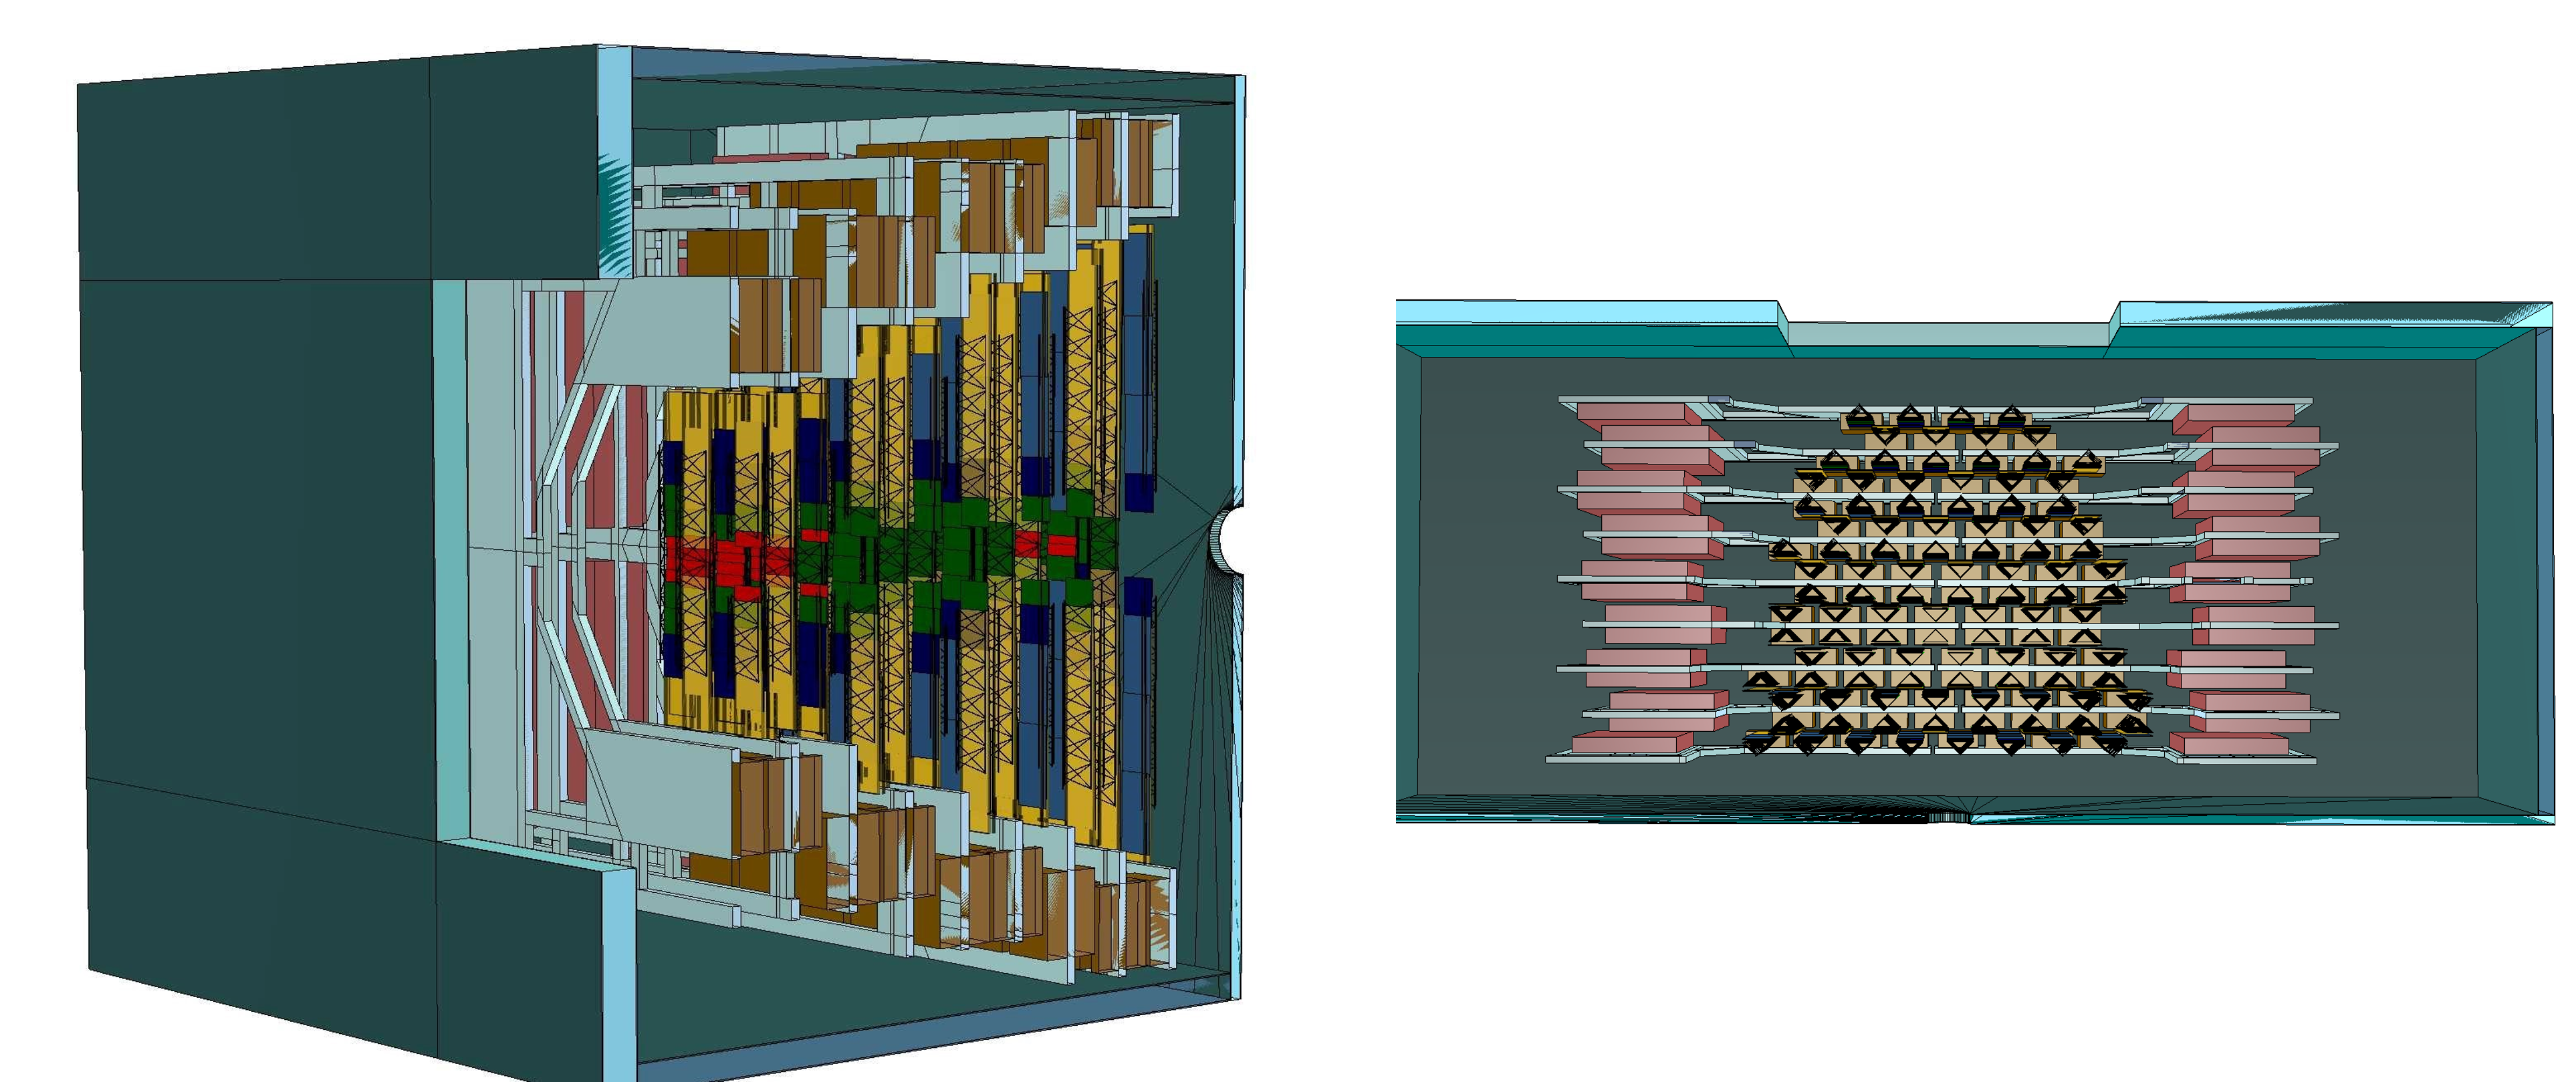
\includegraphics[width=0.85\columnwidth]{Chapter2/images/STS.png}
\caption{A simplified geometry of the Silicon Tracking System. The 8 tracking stations cover the polar angle from \SI{2}{\degree} up to \SI{25}{\degree}.}
\label{fig_STS}
\end{figure}

The detector consists of 876 detectors modules. A module is composed of double-sided silicon microstrip sensors, ultralight microcables (of up to 50~cm length) and Front End Boards (\gls{FEB}) populated with ASICs (STS-XYTER) glued on the fins. The modules are distributed on carbon fiber support-structures which populate C-frames~\cite{progress_report_2016}. Two C-frames form a tracking station of \gls{STS}.  Figure~\ref{fig_assembly} depicts a simplified assembly workflow of \gls{STS}.
The modules are produced in 166 variants, which differ in sensors size, micro-cable length and the orientation of the Front End Electronics~(\gls{FEE}).  


The stations are placed inside a thermally insulated box which resides in a dipole magnet. During \gls{STS} operation, the temperature inside the enclosure will be gradually decreased with the increasing radiation damage to the silicon sensors, to ensure no risk of thermal runaway~\cite{Spieler}. In principle, the largest amount of heat is dissipated by the low-voltage powering of the electronics and not the sensors themselves. Hence, an effective cooling is needed to address this problem.
The temperature of about \SI{-10}{\celsius} will ensure a safe performance of the semiconductors and minimize the contribution of the shot noise~\cite{Spieler}. The low ambient temperature also sets hard limits on the frost point. As the coolant temperatures might reach down to \SI{-40}{\celsius}, the frost point needs to be below \SI{-45} at all times. 

\newpage
\begin{figure}[!h]
\centering
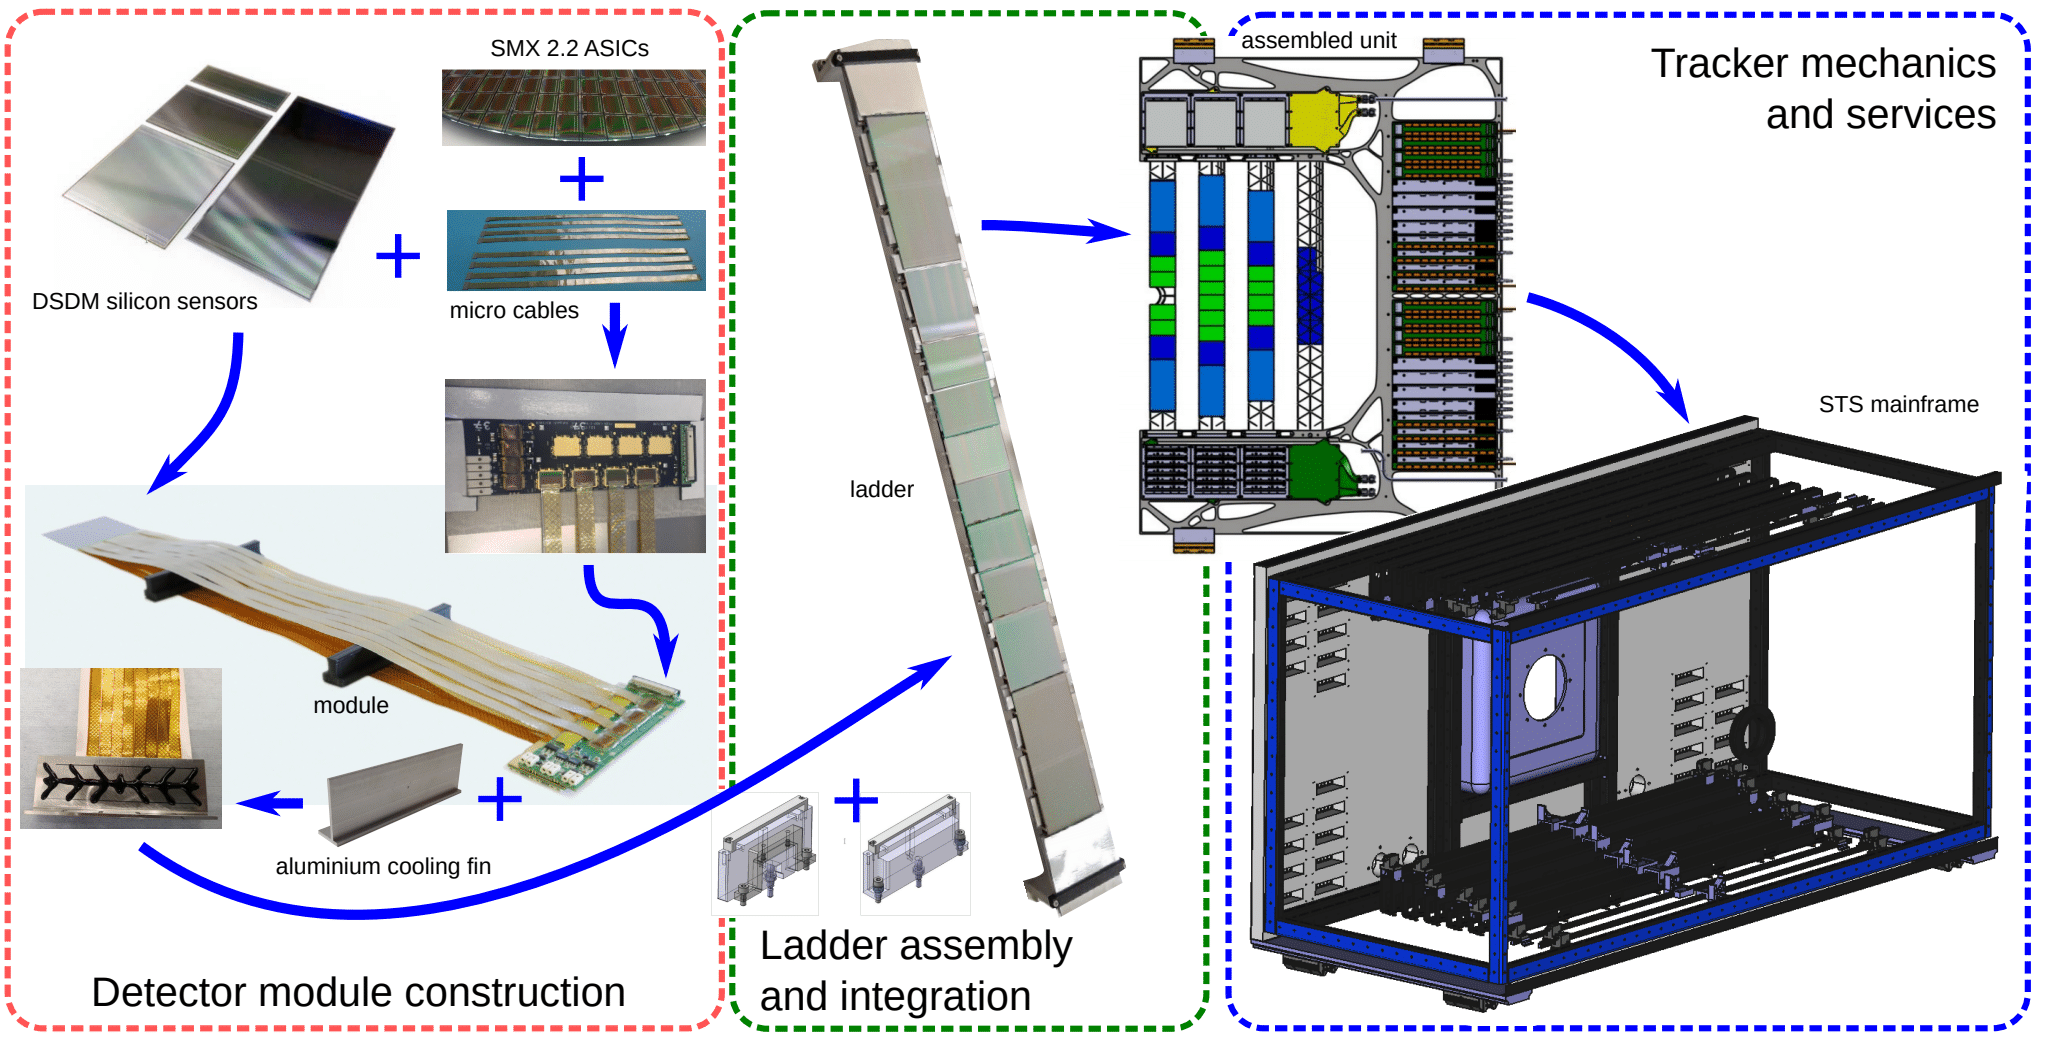
\includegraphics[width=1\columnwidth]{Chapter2/images/assembly_sequence.png}
\caption{A simplified assembly workflow of the \gls{STS}. The silicon sensors are connected to the ASICs on the \glspl{FEB} via microcables. The modules are assembled into carbon fiber ladders which form a C-frame. (Private information from M. Teklishyn)}
\label{fig_assembly}
\end{figure}

%The evolution of different experimental setups constructed for the purpose of testing components of the \gls{STS} is depicted in Figure \ref{fig_evolution_STS}. 

%\begin{figure}[!h]
%\centering
%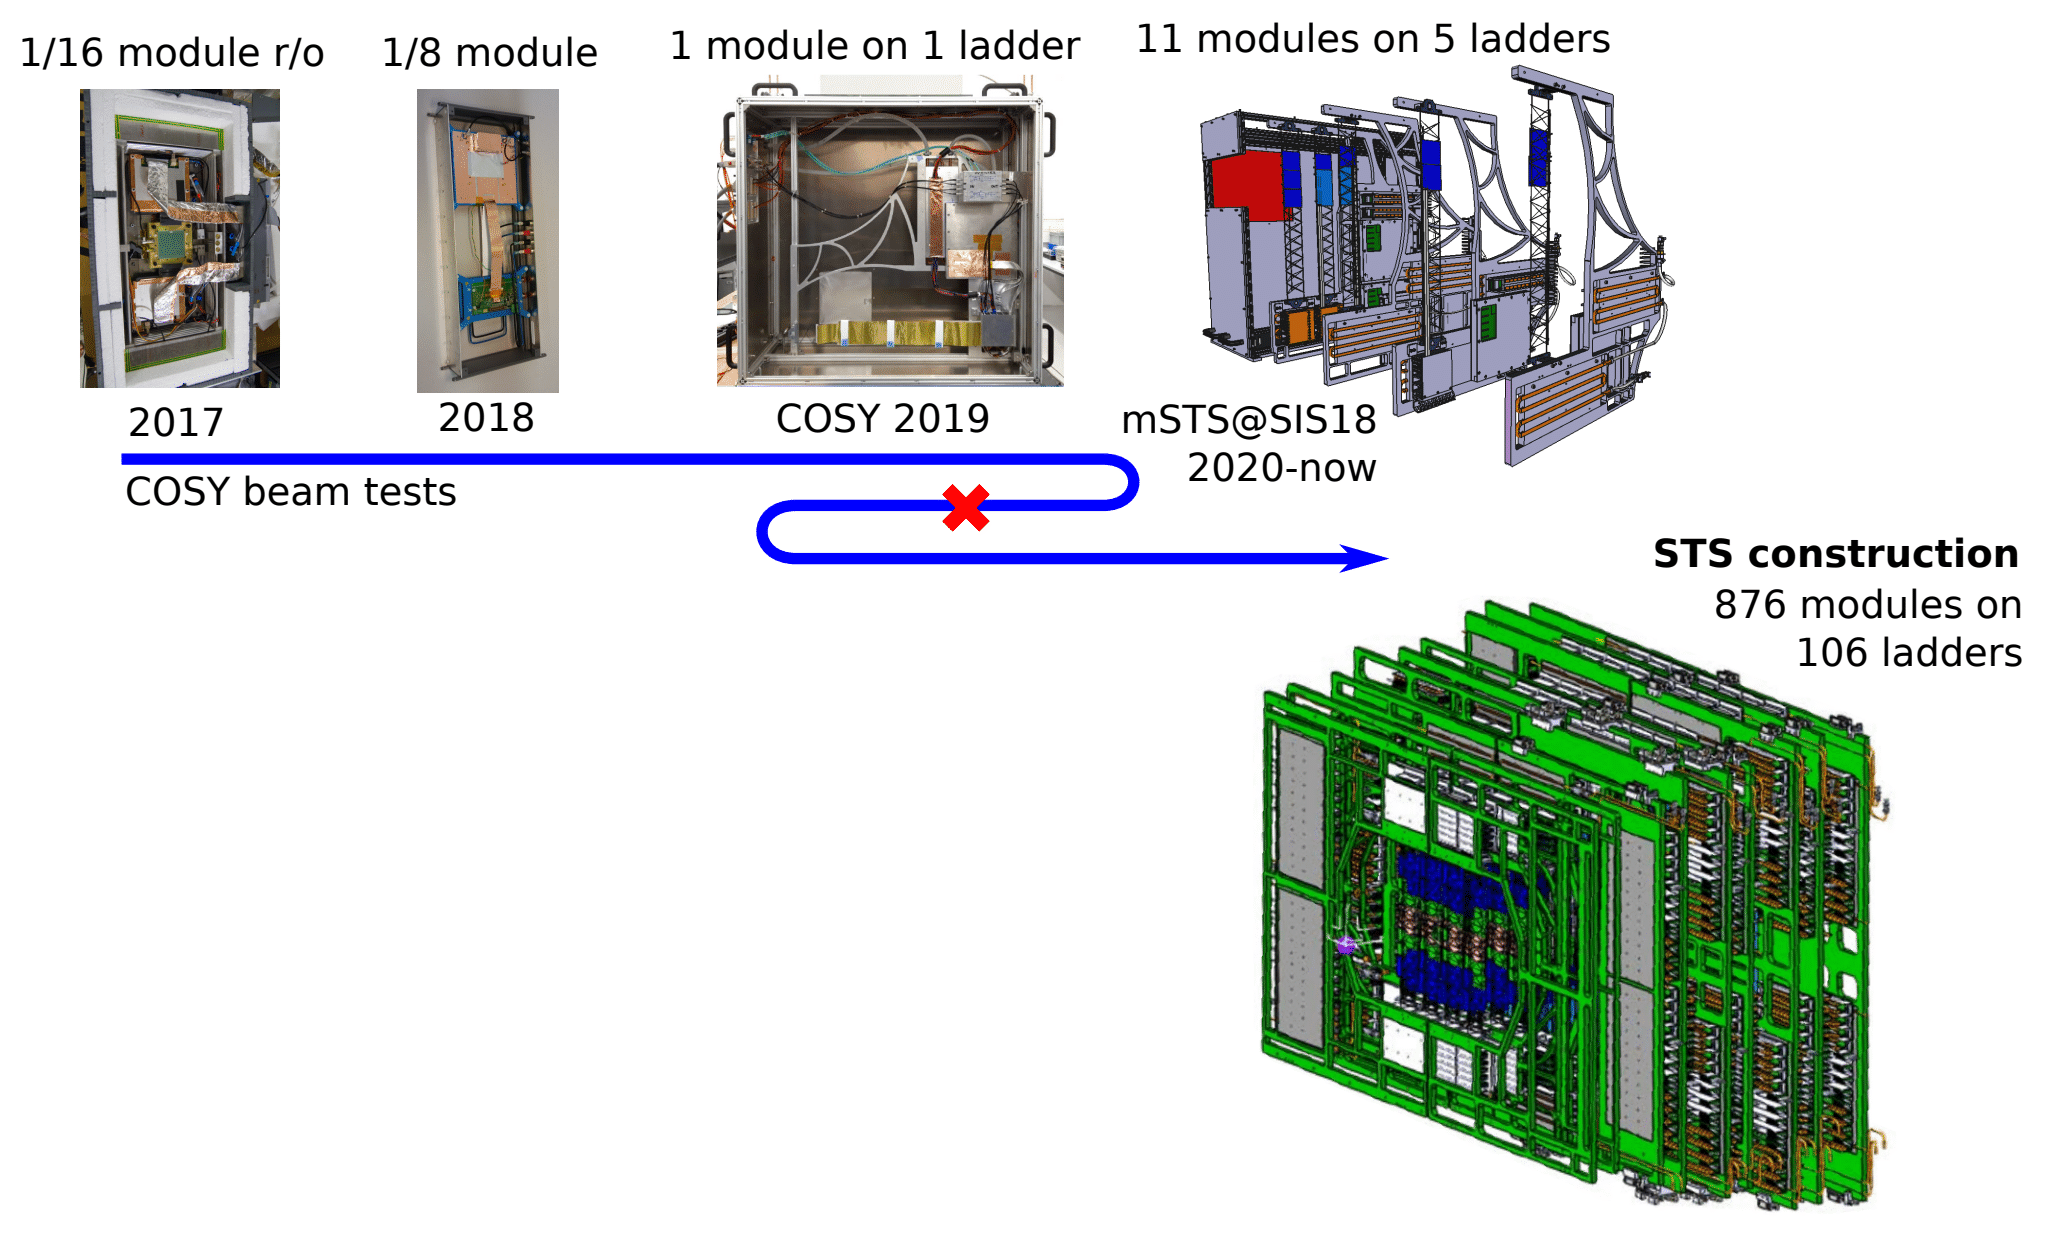
\includegraphics[width=0.95\columnwidth]{Chapter2/images/evolution_sts_new.png}
%\caption{Evolution of the test setups towards \gls{STS}. (Private information %from M. Teklishyn)}
%\label{fig_evolution_STS}
%\end{figure}




\subsection{Double-sided microstrip silicon sensors}
\label{sensors}

The use of microstrip silicon sensors has been demonstrated in many well-known experiments like those operated at \gls{CERN}(\gls{ALICE} and \gls{CMS}) and Brookhaven National Laboratory (\gls{STAR}). The aluminum strips on the p-side of the sensors are inclined by \SI{7.5}{\degree} with respect to the n-side. That implies that there is a set of shorter strips on the p-side. These strips are interconnected with each other using a second metallization layer on the sensors. An example of this solution is presented in Figure~\ref{fig_sts_si}. 

\begin{figure}[!h]
\centering
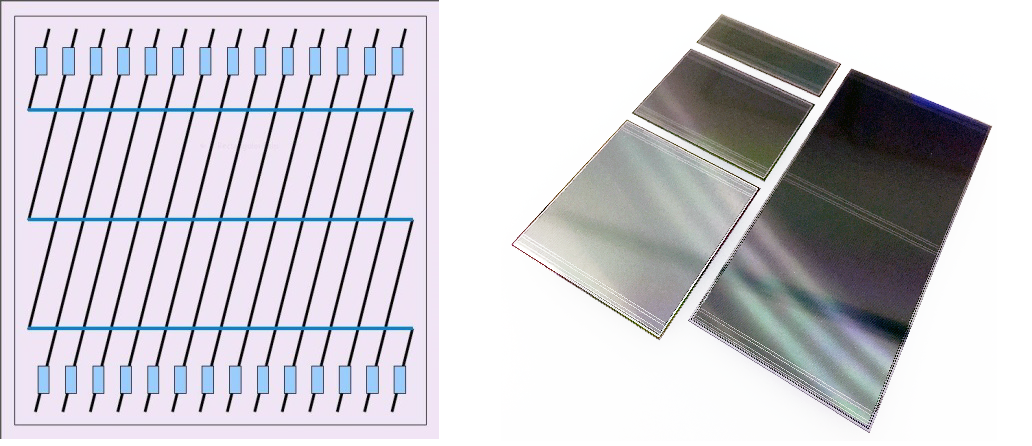
\includegraphics[width=0.75\columnwidth]{Chapter2/images/silicon_sensors.png}
\caption{Left: An example of sensor's electrode segmented into strips inclined by a small angle. The shortest strips are interconnected with each other. Right: The silicon sensors to be used for the \gls{STS}. The width of the sensor is \SI{6.2}{\centi\metre} and there are 4 strip lengths: \SI{2.2}{\centi\metre}, \SI{4.2}{\centi\metre}, \SI{6.2}{\centi\metre}, \SI{12.4}{\centi\metre}.}
\label{fig_sts_si}
\end{figure}

The sensors are produced on \SI{320}{\micro\metre} thick n-type wafers by Hamamatsu Photonics K.K. Each of the sensors features 1024 strips with \SI{58}{\micro\metre} pitch. The signal from the sensors is transported to the front-end electronics via ultra-light microcables. These cables are additionally shielded to protect the analog signals from any interference. 

\subsection{Module}
\label{module}
 The assembly of the detector is realized stepwise. The whole complex procedure requires utmost care and extremely high precision. Therefore, a proper workflow was developed to address the complexity of the module assembly~\cite{carmen2}.

\subsection{The readout chain of the STS}
\label{readout}
\label{DAQ}
The \gls{STS} readout chain is designed to control, readout and preprocess analog signals acquired from the silicon sensors. Moreover, it has to handle a high data throughput and store it. The \gls{CBM} experiment is going to run with a free-streaming Data Acquisition (\gls{DAQ}) system. It is made of the \gls{FEE}, data transport, online event reconstruction and online event selection~\cite{Kasinski1}.

The first layer of the \gls{STS}'s readout chain consists of Front-End Board (\gls{FEB}) which is populated with 8  Application-specific integrated circuits (ASICs)~\cite{Kasinski2}. Each ASIC or STS-XYTER is responsible for readout of 128 channels. The chips feature the analog front-end (\gls{AFE}), the digitizer and generation of hits using Analog Digital Converter (\gls{ADC}) and timestamp information. 

The next element, which transports data from the \gls{FEE} is the readout board (\gls{ROB}). It aggregates data from multiple \glspl{FEB} and sends it via optical links out of the detector enclosure to the Common Readout Interface (\gls{CRI}) board. Subsequently, the data is transported to the First Event Level Selector (\gls{FLES}). 

In total, the \gls{STS} features roughly, 14000 STS-XYTERs, 600 \glspl{ROB}. Given a typical average raw event size of roughly 50 kB for minimum-bias Au+Au collisions, a peak collision rate of 10~MHz results in an instantaneous raw data rate of about 500~GB/s (for the all the detector systems).

\begin{figure}[!h]
\centering
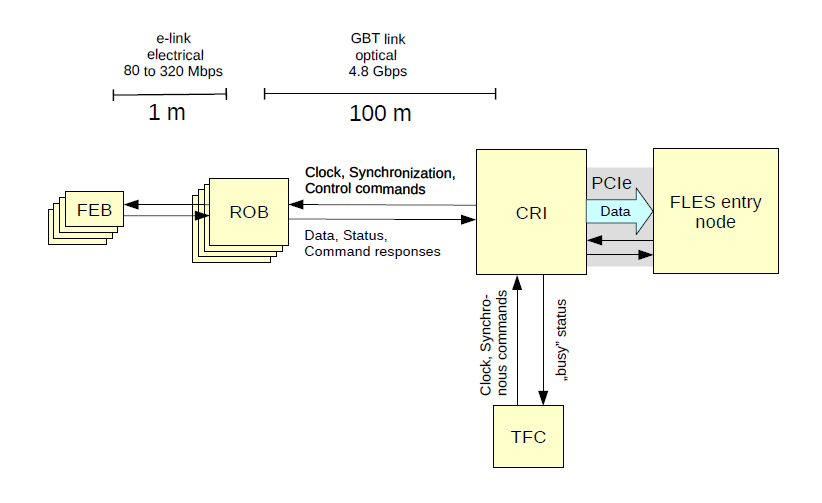
\includegraphics[width=0.8\columnwidth]{Chapter2/images/CRI_DAQ.png}
\caption{The basic building parts for one \gls{FLES} entry node are shown schematically. An entry node can hold many \glspl{CRI}. A \gls{CRI} often serves numerous \glspl{ROB}, whereas a \gls{ROB} typically serves multiple \glspl{FEB}. The Timing and Fast Control (\gls{TFC}) is a core system that is shared by all \glspl{CRI}.}
\label{fig_daq_cri}
\end{figure}

The testing phase features two other readout chains, which are based on Data Processing Board (\gls{DPB}) and GBTxEMU board. 
\subsubsection{STS-XYTER}

\subsubsection{Front-end boards (FEB)}

\subsubsection{Readout board (ROB)}

\subsubsection{Common Readout Interface (CRI)}
\subsection{Alternative readout chains for testing purposes}

\subsection{DPB-based readout chain}

\subsection{Tester readout chain}

There are three main readout chains that have been exercised for different detector development activities.  
The readout chain used in the module or FEBs test is built from two components: 
\begin{enumerate}
    \item the Common Readout Board (\gls{CROB}) for data concentration and transport with electrical to optical interface (see figure 
    \item Data Processing Board (DPB) based on the AFCK board (see Fig.
\end{enumerate}

\begin{figure}[!h]
\centering
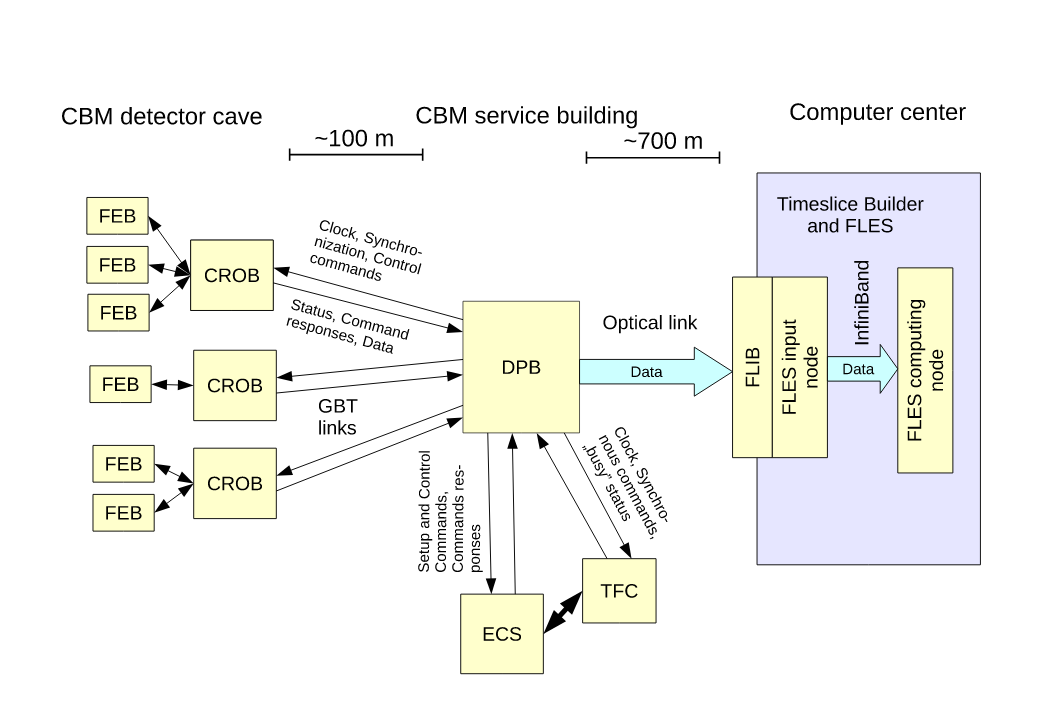
\includegraphics[width=0.75\columnwidth]{Chapter2/images/DPB.png}
\caption{The first proposition of the CBM readout chain based on separate DPB and FLIB boards \ref{fig_cri_board}}
\label{fig_dpb_scheme}
\end{figure}

\begin{figure}[!h]
\centering
\includegraphics[width=0.65\columnwidth]{Chapter2/images/feb_8_v2.pdf}
\caption{FEB}
\label{fig_febA_photo}
\end{figure}
\subsection{CRI based readout chain}
\begin{figure}[!h]
\centering
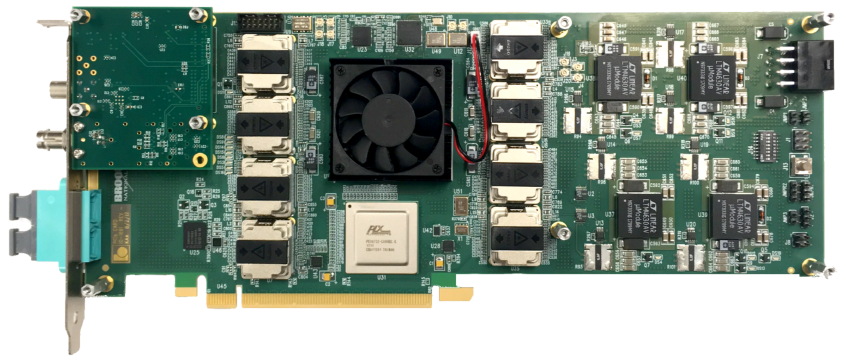
\includegraphics[width=0.65\columnwidth]{Chapter2/images/cri_board_atlas.pdf}
\caption{CRI board}
\label{fig_cri_board}
\end{figure}

\label{tester}
Another alternative to the two readout chains introduced in the last two sections is the so-called GBTxEMU-based tester. It is based on a commercial Artix-7 board (TE-0712, Trenz Electronics Gmbh), and allows emulating GBTX ASIC or the whole CROB. Moreover, it could also be used in an autonomous mode with the addition of VITA  57.1 FMC adapter
\subsection{Powering schematics of the detector}
\label{powering}
\subsection{Cooling concept for the STS's electronics and silicon sensors}
\label{cooling}


\section{Requirements for the control system}
\label{sys:req}
Custom solutions that are applied in \gls{STS} make the control of this system very challenging. Different services imply different control solutions which need to be implemented.
A distributed control system should offer remote control, alarm detection, reporting and logging, modeling and simulation, data processing (archiving, retrieval, plotting, conversion, analysis), common time management, access security, and automatic \footnote{Sequencing, also known as sequential control, it controls the device in a pre-determined order.}{sequencing}.
In addition to that, the \gls{DCS} for the Silicon Tracking System (\gls{STS}) is being designed taking into consideration the following aspects:

 
 \begin{itemize}
    \item potential control framework should offer the possibility to control a variety of different services, which often have different communication protocols,
    \item logging, and monitoring - there should be reliable means of supervision of processes, containers, and \footnote{The input/output controller is a device that interfaces between an input or output device and the computer or hardware device}{Input/Output Controllers} (\glspl{IOC}).
    \item the control software should be horizontally and vertically scalable, when it comes to adding additional computing nodes or applications/Input Output Controllers (\glspl{IOC})/containers,
    \item supervision - it should be possible to integrate a sub-system oriented with higher-level control structures,
     \item flexible - applications should be easy to run on different operating systems and processor architectures,
     \item sustainability and support - the experiment is supposed to run for about 10 years, excluding the building and commissioning time. The control system should be sustainable and long-term support provided,
     \item reliability - the system should be highly available, minimizing the downtimes,
     \item network separation - it should be running in a dedicated network (divided into several service-oriented subnets) to have a good overview of the processes and communication between the nodes,
     \item \glspl{GUI} - all parameters/\footnote{In control theory, a process variable is the currently measured value of a particular part of a process which is being monitored or controlled}{process variables} should be available in a user-friendly Graphical User Interface (\gls{GUI}). In case of error or malfunction, it should be stated clearly by the software where the error happened, what could be the potential risk and what actions need to be taken.

 \end{itemize}
\newpage


\chapter{DCS, an important part of the online systems}
\label{chap:online_systems}

As mentioned in the previous chapter, the \gls{CBM} will face an unprecedented interaction rate in high-energy physics experiments (up to $10^{7}$~events/s). That number sets also a clear requirement for the detector systems and their corresponding data acquisition. Moreover, due to the huge quantity of incoming data which is closely connected to the storage size, certain design decisions had to be made in order to reduce the raw data coming from the subsystems. To address \gls{CBM} conditions complex triggers would have to be introduced, e.g. signatures of off-target decays of $\Omega$ hyperons. The decay topologies required for the reconstruction of the collisions imply a long trigger latency~\cite{Friese_2017}. In order to realize such a complex trigger logic and reduce the data amount, the raw data needs to be evaluated in software on \glspl{CPU} and/or \glspl{GPU}. The self-triggered readout system implies that the association of data from different detectors to physical collision events must be based solely on their timestamp, which is generated in the frond-end electronic (\gls{FEE}) circuitry. As a result, a central timing system must synchronize the \gls{FEE} elements to sub-nanosecond precision. On the other hand, the typical "event building" action and the high-level trigger are transitioned to the \gls{FLES} ("First-level Event Selector") online compute farm. 

\begin{figure}[!h]
\centering
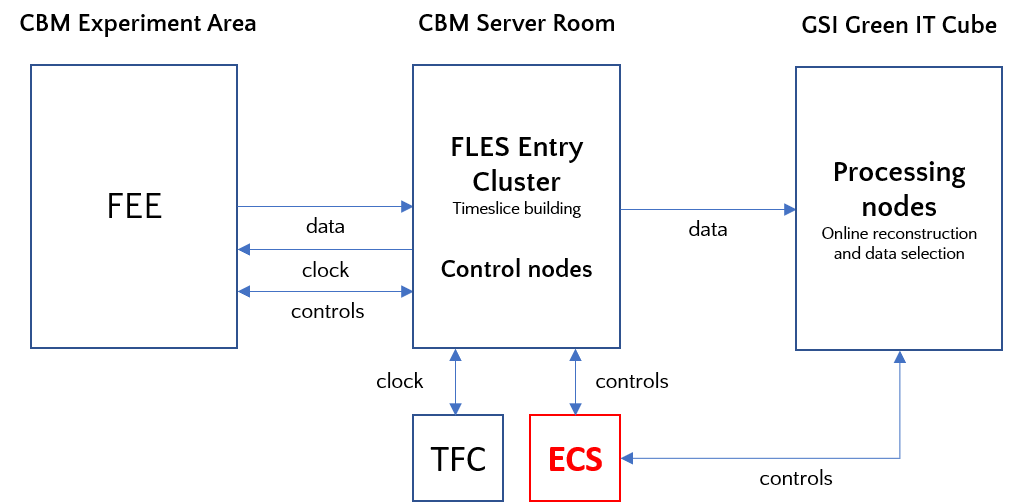
\includegraphics[width=0.8\columnwidth]{Chapter3/Controls/images/online.png}
\caption{Schematics of the CBM readout systems}
\label{fig_controls}
\end{figure}

The readout hardware is connected to the farm via custom-developed optical links that manage clock and time distribution, data transfer, and control communication. The Common Readout Interface (\gls{CRI}) connects the links to the online farm. The CRI forwards the clock and time information obtained from the Timing and Fast Control (\gls{TFC}) system to the detector \gls{FEE}, and also converts the data received from the detector. Figure~\ref{fig_controls} shows the schematic view of the controls and data acquisition chain of the \gls{CBM} experiment. The Experiment Control System (\gls{ECS}) highlighted in red is also the supervisory structure of the Detector Control System (\gls{DCS}) which controls and monitors the subsystems. The next sections focus on the software components related to the \gls{ECS}, and a detailed explanation of the experiment control with its design. Nevertheless, the main focus is put on the \gls{DCS}.
%\newpage
\section{How to control a HEP experiment?}

Modern \gls{HEP} experiments require complex control systems which are crucial to the successful operation of the installment. Proper implementation of such systems ensures higher safety margins and enhanced data production quality. 
Figure \ref{fig_sim} depicts the targeted controls architecture of the future \gls{CBM} experiment. It consists of different \footnote{A software agent is a persistent, goal-oriented computer program}{software agents} with clearly defined tasks. During the Phase - 0 experiment of the \gls{CBM} (\gls{mCBM}) some parts of the future \gls{ECS} were tested. The respective parts of the controls have been tested in a standalone mode, which means that there hasn't been any structured communication between \gls{DCS}, Device Control Agent (\gls{DCA}), and Experiment Control System (\gls{ECS}). Nevertheless, for the final experiment the detector control system should provide the information on the detector state to the agent(s) residing at a higher position in the control hierarchy, and also request the state of the~\gls{DAQ}.
\begin{figure}[!h]
\centering
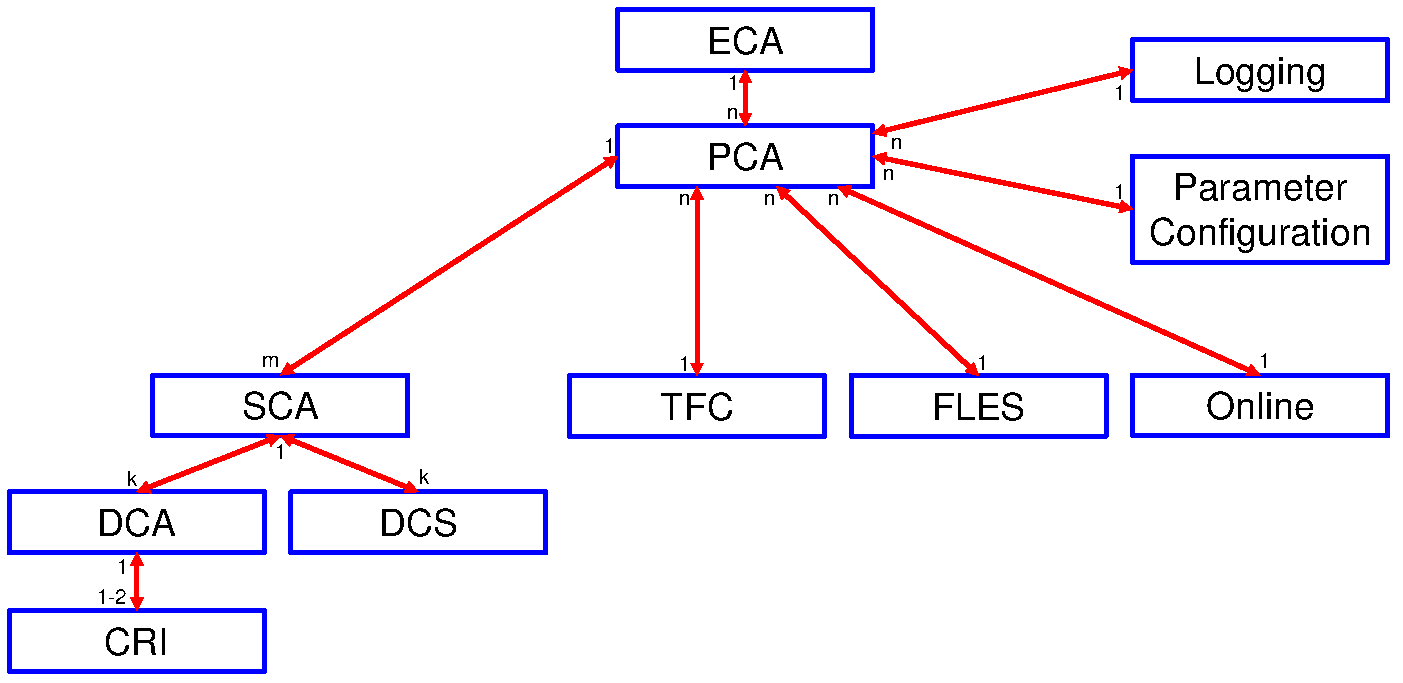
\includegraphics[width=0.8\columnwidth]{Chapter3/Controls/images/AgentsRelations_V2.pdf}
\caption{\gls{ECS} core agent relations}
\label{fig_sim}
\end{figure}

 In the next sections, the main features of the control agents are discussed, in particular those that can influence \gls{DCS} (Partition Control Agent (\gls{PCA}), System Control Agent (\gls{SCA}), and \gls{DCA}). Apart from the mentioned agents, the following components are expected to run: 
 \begin{itemize}
     \item Logging and monitoring system - state or configuration changes should be documented for possible revision,
     \item First Event Selector network - \gls{DAQ} software controlling the data readout and timeslice building,
     \item Online processing - software receiving the data from the FLESnet and processing it,
     \item Time and Fast Control (\gls{TFC}) - hardware source of timing information.
 \end{itemize}
\section{Experiment Control System}\label{sssAgents}

The highest supervisory element of the control strategy is the Experiment Control Agent 
(\gls{ECA}). It is the top layer of the \gls{ECS} core, which should be constantly running and keeping track of the  partitions, of the systems in partitions, and of the systems out of partitions. Partition is a component of the \gls{ECS} describing the combined state of a set of detector systems participating in a common readout. It is used to segment the readout and data flow. It also manages the states of "Central systems," which do not have partition-level states (e.g. \gls{TFC}, \gls{FLES} in case it does not use internal partitions).  It provides the address and port required by agents to establish the \footnote{asynchronous messaging library \cite{zeromq}}{0MQ} sockets and build the \gls{ECS} structure upon request. The \gls{PCA}, is the bottom layer of the \gls{ECS}, which tracks the state and controls a set of detector systems plus all needed central systems. Multiple partitions can run concurrently, potentially allowing for parallel runs with independent detector system sets. 

The \glspl{PCA} also hold internal instances of the necessary System Control Agent \gls{SCA} interfaces, which are responsible for:
\begin{itemize}
 \item holding a copy of the current state of the \gls{SCA},
 \item periodic ping of the \gls{SCA} to ensure early disconnection detection,
 \item sending requests to the \gls{SCA} and receiving the replies,
 \item Monitoring the \gls{SCA} broadcast channel for unexpected/unrequested state changes.
\end{itemize}
These should not be confused with the \gls{SCA}, which are in separate processes (the list will be dynamic and generic at \gls{PCA} level, and can depend on the systems participating in the readout activities):

\begin{itemize}
 \item Time zero (T0), also known as Start Detector or Beam Monitor \gls{BMON})
 \item Micro-Vertex Detector (\gls{MVD})
 \item Silicon Tracking System (\gls{STS})
 \item Ring Imaging CHerenkov (\gls{RICH})
 \item MUon CHambers (\gls{MUCH})
 \item Transition Radiation Detector (\gls{TRD})
 \item Time Of Flight (\gls{TOF})
 \item Beam Fragment Timing Counter (\gls{BFTC})
 \item Projectile Spectators Detector (\gls{PSD})
\end{itemize}

\subsection{System Control Agent and its role}
The subsystem-specific \gls{SCA} should manage communication both with the detector-specific agents and with the higher supervisory entities of the \gls{ECS}. Moreover, the \gls{SCA} should provide higher control levels with the global state whenever it's requested, handle any changes reported by a detector (tracking the state), and provide an interface for the shift crew to monitor the state of the system. 

Two main links of the \gls{SCA} include:
\begin{itemize}
    \item Detector control system - \gls{EPICS} based distributed control system which controls and monitors all the hardware connected to the specific detector,
    \item Device Control Agent (\gls{DCA}) - this agent controls almost all logic on the \gls{CRI} board (excluding the \gls{FLIM} section and direct memory access data path). \gls{DCA} provides a high-level interface for the higher layers of the control architecture, collectively referred as \gls{EDC}. 
\end{itemize}











\section{Introduction to controlling a detector}
A robust, well-defined control system is a compulsory element for every complex experimental setup, especially in radiation-controlled areas. To ensure the safe operation of a detector subsystem, automation processes are commonly implemented (e.g., in the form of a Finite State Machine\footnote{A state of the Finite State Machine is clearly defined at any given point in time. It can move to another state by processing an input.} (\gls{FSM}) or hardware interlocks). In the \gls{STS} case, to ease the use and implementation of a control system, a fairly novel approach was used. It is primarily based on the containerization\footnote{Containerization is the packaging of software code with just the operating system libraries and dependencies required to run the code.} of different applications used to monitor and control setups. 

%\begin{figure}[!h]
%\centering
%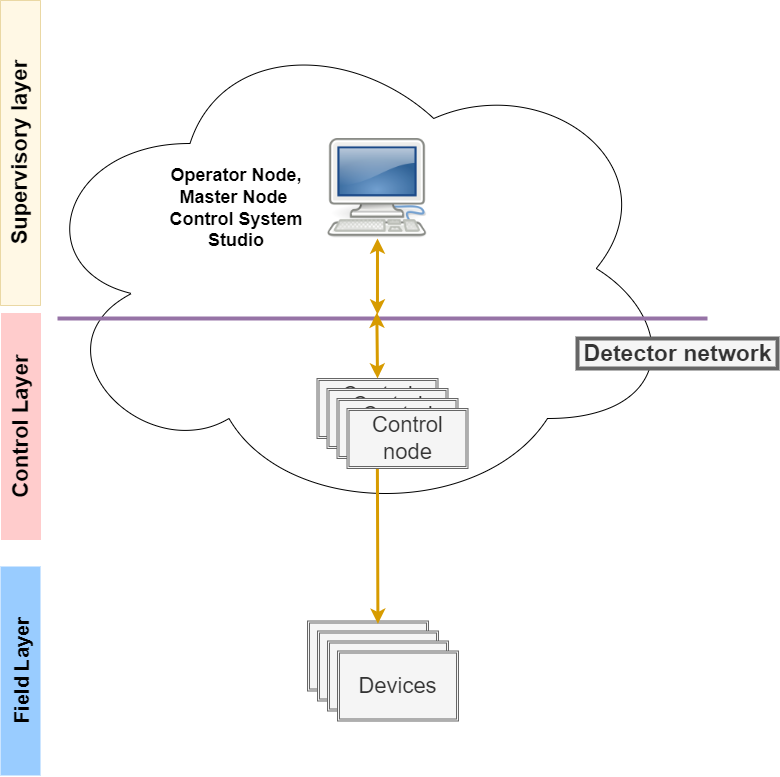
\includegraphics[width=0.55\columnwidth]{Chapter3/Controls/images/example.png}
%\caption{General detector control system architecture}
%\label{fig_DCS_arch}
%\end{figure}



A control system must provide multiple functionalities to operate effectively. These include communication between hardware and software layers, visualization of data, logging of system events, archiving of historical data, and controlling means. Control can be automated using a \gls{FSM} or performed manually, depending on the requirements of the system being controlled. The control system can be usually divided into three layers: field layer, control layer, and supervisory layer. The bottom (field) layer contains all the process sensors, actuators, and other devices that are connected to the control system via I/O boards and/or field buses. Communication between the field layer and control layer can be of almost any type compatible with the used components, i.e., Ethernet, Modbus \gls{TCP}, Profibus. The control logic is introduced in the Programmable Logic Controller (\glspl{PLC}) and so-called control nodes (single board computers etc.) in the control layer. The supervision layer or supervisory level provides the operators with means of controlling and monitoring the subsystem, for example via command line or a Graphical User Interface (\gls{GUI}) or Operator Interface (\gls{OPI})~\cite{layers}.  Typically, DCS building blocks reside in a dedicated network to avoid unnecessary cross-talk and ensure more efficient debugging.

Figure \ref{fig_arch} shows a general idea behind the \gls{STS} \gls{DCS} from the software point of view.  The master node or the central \gls{DCS} node receives data from the configuration database, which allows the preparation of subsystems for a given action (for example, for a transition into a different state). The master node will be only accessible by the \gls{DCS} experts, excluding subsystem-related personnel from performing actions on other subsystems \gls{DCS}. There are also one or more archiving nodes and control nodes, which will contain detector-specific applications. All the mentioned components allow effective control over a detector and deliver crucial operational information (alarms, events, Process Variables (\glspl{PV}) values, etc.). 

\begin{figure}[!h]
\centering
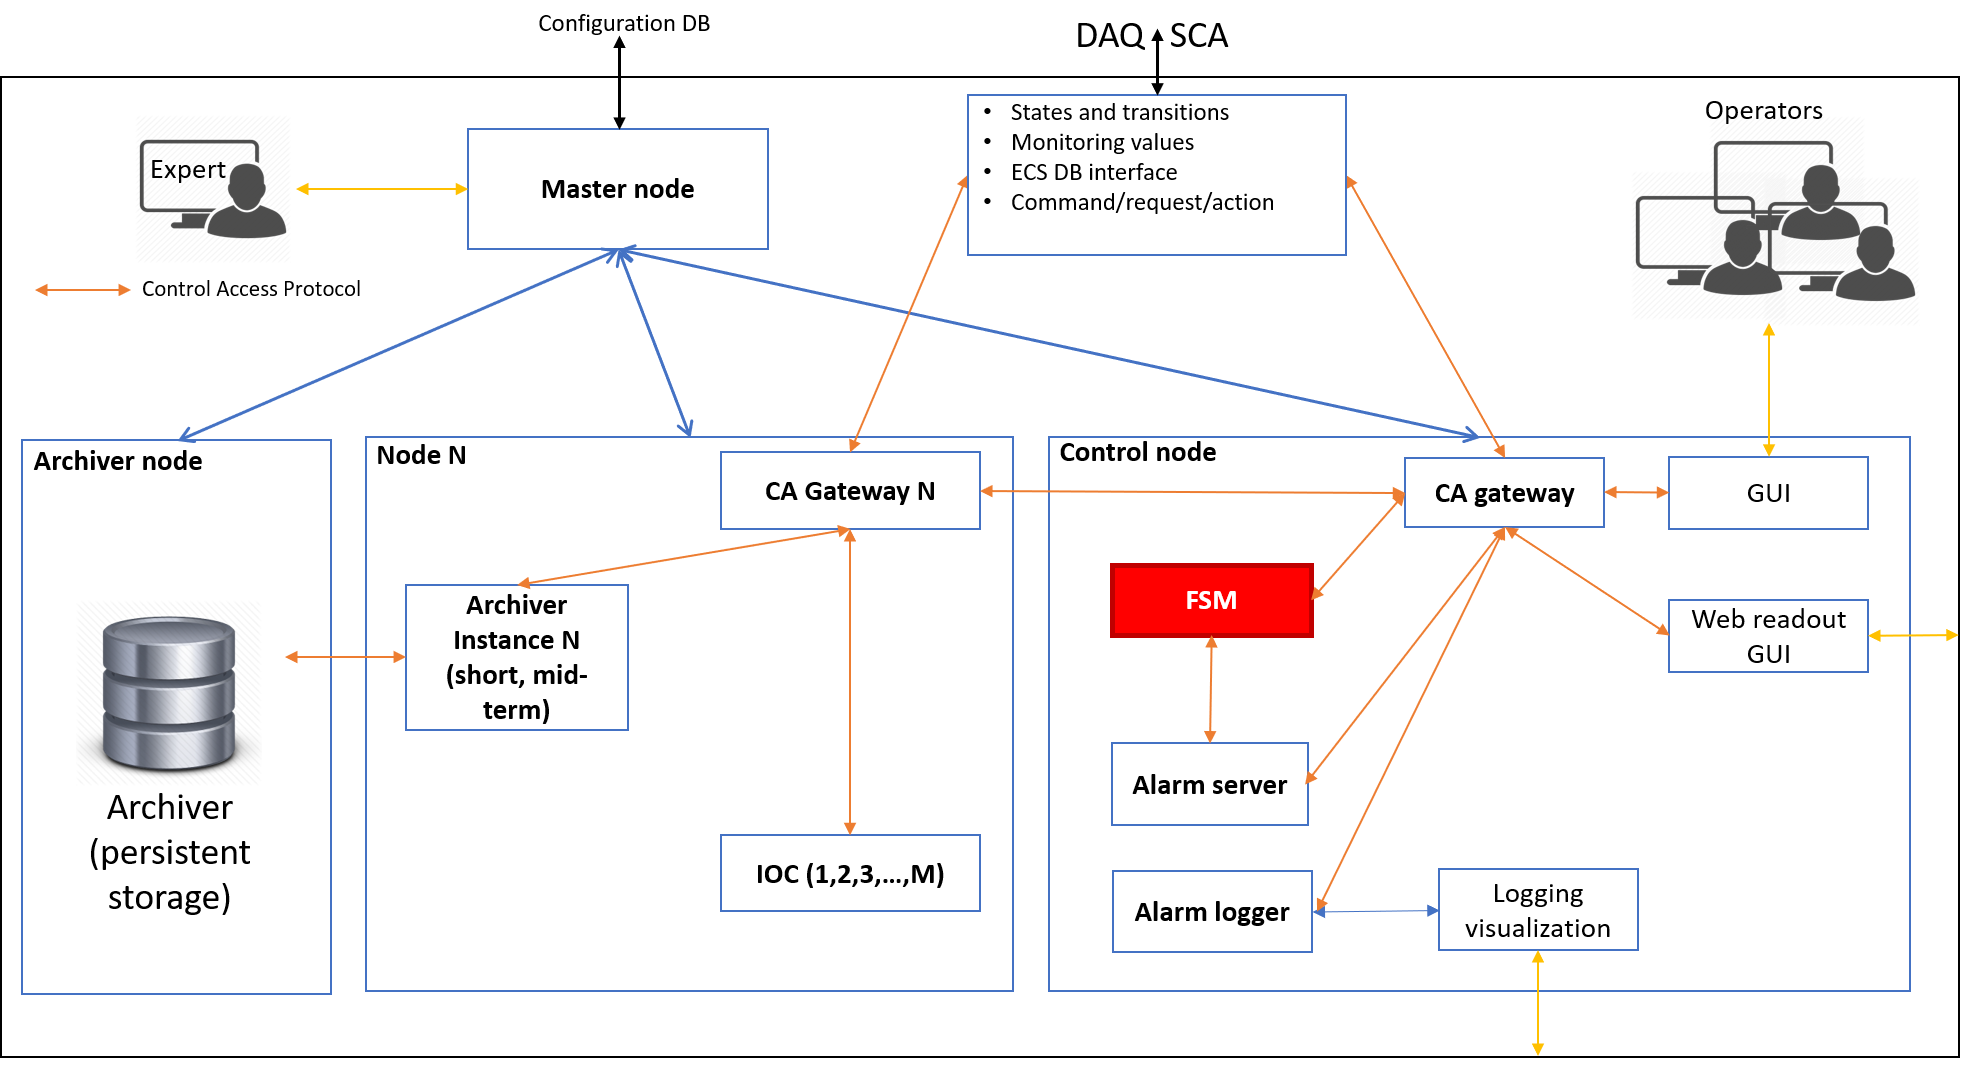
\includegraphics[width=1\columnwidth]{Chapter3/Controls/images/DCS.png}
\caption{Proposed \gls{DCS} infrastructure for the \gls{STS}. The scheme describes the most important software components including the archiver, alarm server, alarm logger, GUIs, \glspl{FSM}, and corresponding interfaces.}
\label{fig_arch}
\end{figure}
\newpage







%empty page
%\newpage
%\thispagestyle{empty} 
%\mbox{}

%\clearpage
%\pagenumbering{arabic}


%%% Insert here the text body, replacing the dummy content.
%\label{sec:introduction
\subsection{Control system for the CBM experiment}
The \gls{EPICS} was chosen, as a system that answers most of the needs for the future \gls{DCS} of the \gls{CBM} experiment. More detailed explanations of how \gls{EPICS} works are described in the next sections. According to \cite{EPICS_DOCS}, the basic attributes of \gls{EPICS} are:
\begin{itemize}
    \item tool based - minimized need for custom coding,
    \item distributed - an arbitrary number of \glspl{IOC} and \glspl{OPI}, as long as the network doesn't saturate,
    \item event driven - it's designed to be event-driven to the maximum extent possible,
    \item high performance, robust,
    \item scalable,
    \item under constant development (see latest updates related to the Control System Studio and PVA)
\end{itemize}




%\section{How to control a detector?}

\subsection{What is EPICS?} 
\label{EPICS}
EPICS is a set of tools and applications which provide a software infrastructure for distributed control systems \cite{EPICS_license}. This framework could be used for large systems like particle accelerators, telescopes, etc. as well as for smaller systems featuring only several hundred process variables \cite{EPICS_1, EPICS_2, EPICS_3, EPICS_4}.
\begin{figure}[!h]
\centering
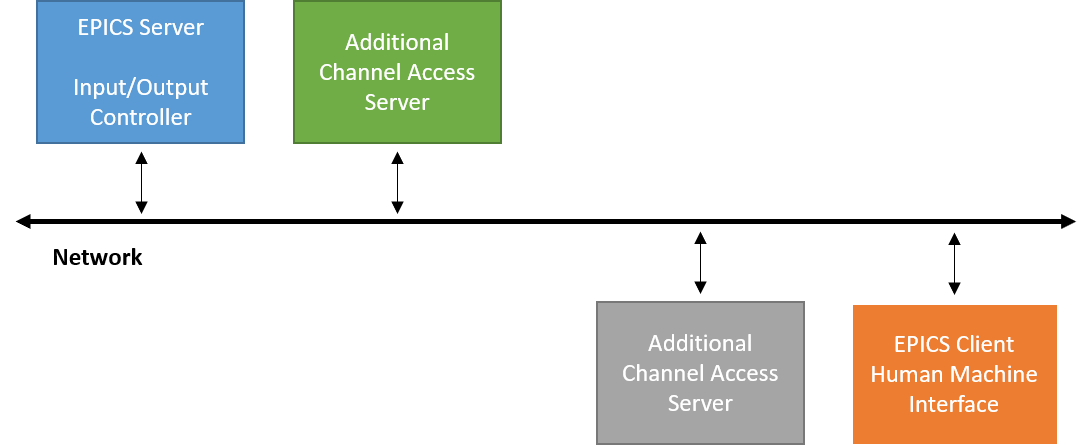
\includegraphics[width=0.7\columnwidth]{Chapter3/DCS/images/EPICS.png}
\caption{EPICS working principle}
\label{fig_EPICS}
\end{figure}
As described in Figure \ref{fig_EPICS}, the system uses Client/Server and Publish/Subscribe approaches to communicate between different devices/nodes. Most servers, called Input/Output Controllers ( \gls{IOC}) perform I/O and local control tasks and publish this information to clients via dedicated protocols Channel Access and/or pvAccess \cite{EPICS}. 

 \subsection{Available control tool sets}
 EPICS and related toolkits offer a complete set of applications to control large experiments. Many different sites all over the world have implemented EPICS-based control systems, i.e. \gls{J-PARC} \cite{J-PARC}, \gls{STAR} \cite{STAR}, \gls{ITER} \cite{ITER}, Australian Synchrotron and many more \cite{EPICS_site}.  Nevertheless, there are also different alternatives to implementing a control system, which include: 
 \begin{itemize}
     \item Siemens WinCC \cite{Camacho:2022fxa,Goralczyk:2022udx}
     \item Tango \cite{Santander-Vela:2021tma}
     \item Labview \cite{State:2022qlw} 
     \item custom software (e.g. python/C++ or stream processing software) \cite{taurus}
 \end{itemize} 
 These frameworks were discarded either because of licensing needs (Labview, Siemens WinCC) or lack of extensive experience on-site (Tango). Phoebus \cite{Phoebus} was chosen as the collection of tools and applications to monitor and operate \gls{mSTS}. All \gls{mSTS}'s \glspl{OPI} were prepared in Phoebus \cite{Phoebus}. The detector uses the following Phoebus-related applications:
\begin{itemize}
    \item Alarms logging
    \item Alarm server
    \item Save and restore
\end{itemize}
More details about these applications and their use will be provided in the next sections. Although Phoebus proved to be easy to use and implement new operator screens, there are also alternatives that could provide similar functionalities:
\begin{itemize}
    \item Bluesky Project (Python-based set of libraries \cite{Bluesky})
    \item React Automation Studio \cite{React}
    \item Channel Access Tools - MEDM, \gls{ALH}, \gls{AR} etc. 
\end{itemize}

\subsection{EPICS architecture and IOC}

The heart of the system is an \gls{IOC}, which provides control logic for the connected hardware. An \gls{IOC} contains a few components \cite{IOC}:
\begin{itemize}
    \item \gls{IOC} Database - which contains all the user-defined database  records,
    \item record support - set of support routines defining a record,
    \item Sequencer - an optional extension of the \gls{IOC} which is a finite state machine,
    \item Monitors and scanners,
    \item Channel Access and/or PVAccess (newer protocol added with EPICS7 release),
    \item Device Support and drivers - serve access to external devices
\end{itemize}
An \gls{IOC} doesn't need many computing resources, that's why it runs also on low-power single-board computers like Raspberry PI or Odroid. 
 \gls{IOC} are also commonly supported by additional modules, device support, libraries, and \gls{API}s which altogether provide an efficient way to control various devices.
To communicate with devices, an \gls{IOC} uses so-called device support. The most commonly used ones include:
\begin{itemize}
    \item StreamDevice is a generic EPICS device support for devices with a "byte stream" based communication interface. That means devices that can be controlled by sending and receiving strings (in the broadest sense, including non-printable characters and even null-bytes). Examples of this type of communication interface are serial line (RS-232, RS-485, ...), IEEE-488 (also known as GPIB or HP-IB), and telnet-like TCP/IP \cite{StreamDevice},
    \item devModbus \cite{modbus} - includes support for three Modbus standards (TCP, RTU, ASCII), used for control of climatic chambers in the \gls{STS} group,
    \item asynDriver \cite{asyn} - asynchronous driver support, which is an interface that implements a device-specific code to low-level communication drivers. Together with the StreamDevice it's the most commonly used one in the \gls{mSTS}. 
\end{itemize}

In order to ease the deployment process and have a flexible solution for different architectures, we created images for the \gls{IOC} as well as other \gls{DCS} building blocks. These images can be seen as files with code that upon execution result in the initialization of a container. More detailed information about containerization is included in the next chapter. 
 

\section{Containerized IOC}
\label{containerizer_ioc}
Containerization is an increasingly popular method of virtualizing an application without running a full-blown operating system. In current practices, containers are commonly used both in development and production environments, often together with cloud solutions. In the \gls{HEP} community, containers and their different applications become increasingly popular. According to~\cite{Klaus2021} the first mention of Docker\footnote{Docker is a set of products that use operating system level virtualization to deliver software in packages called containers.} container of the \gls{EPICS} \gls{IOC} was related to the Taurus project in 2015~\cite{taurus}. Since then containerization efforts intensified also within the \gls{FAIR} based collaborations - \gls{CBM}/\gls{MVD}~\cite{Klaus2021} and PANDA DCS~\cite{PANDA_1}.

IOC container has been prepared by the \gls{DCS} group of the \gls{PANDA} Collaboration and adjusted to the \gls{STS} needs. The latest \gls{IOC}'s image is built on EPICS R7.0.3.1 image, and it contains the most important modules and extensions i.a. asyn, autosave, calc, Modbus, and SNMP (see Figure~\ref{fig_ioc1}). By using so-called volumes (see Figure~\ref{fig_doc}) the \gls{IOC} can be used at any node with the Docker engine. Volumes are one of the mechanisms to manage application data, and it's a proper way to ensure data persistence. When a container is started, Docker loads the read-only image layer, adds a read-write layer on top of the image stack, and mounts volumes onto the container file system. Having prepared database files, st.cmd, and stream protocols if needed, an \gls{IOC} can be deployed on any node, with any operating system and processor architecture.
\begin{figure}[!h]
\centering
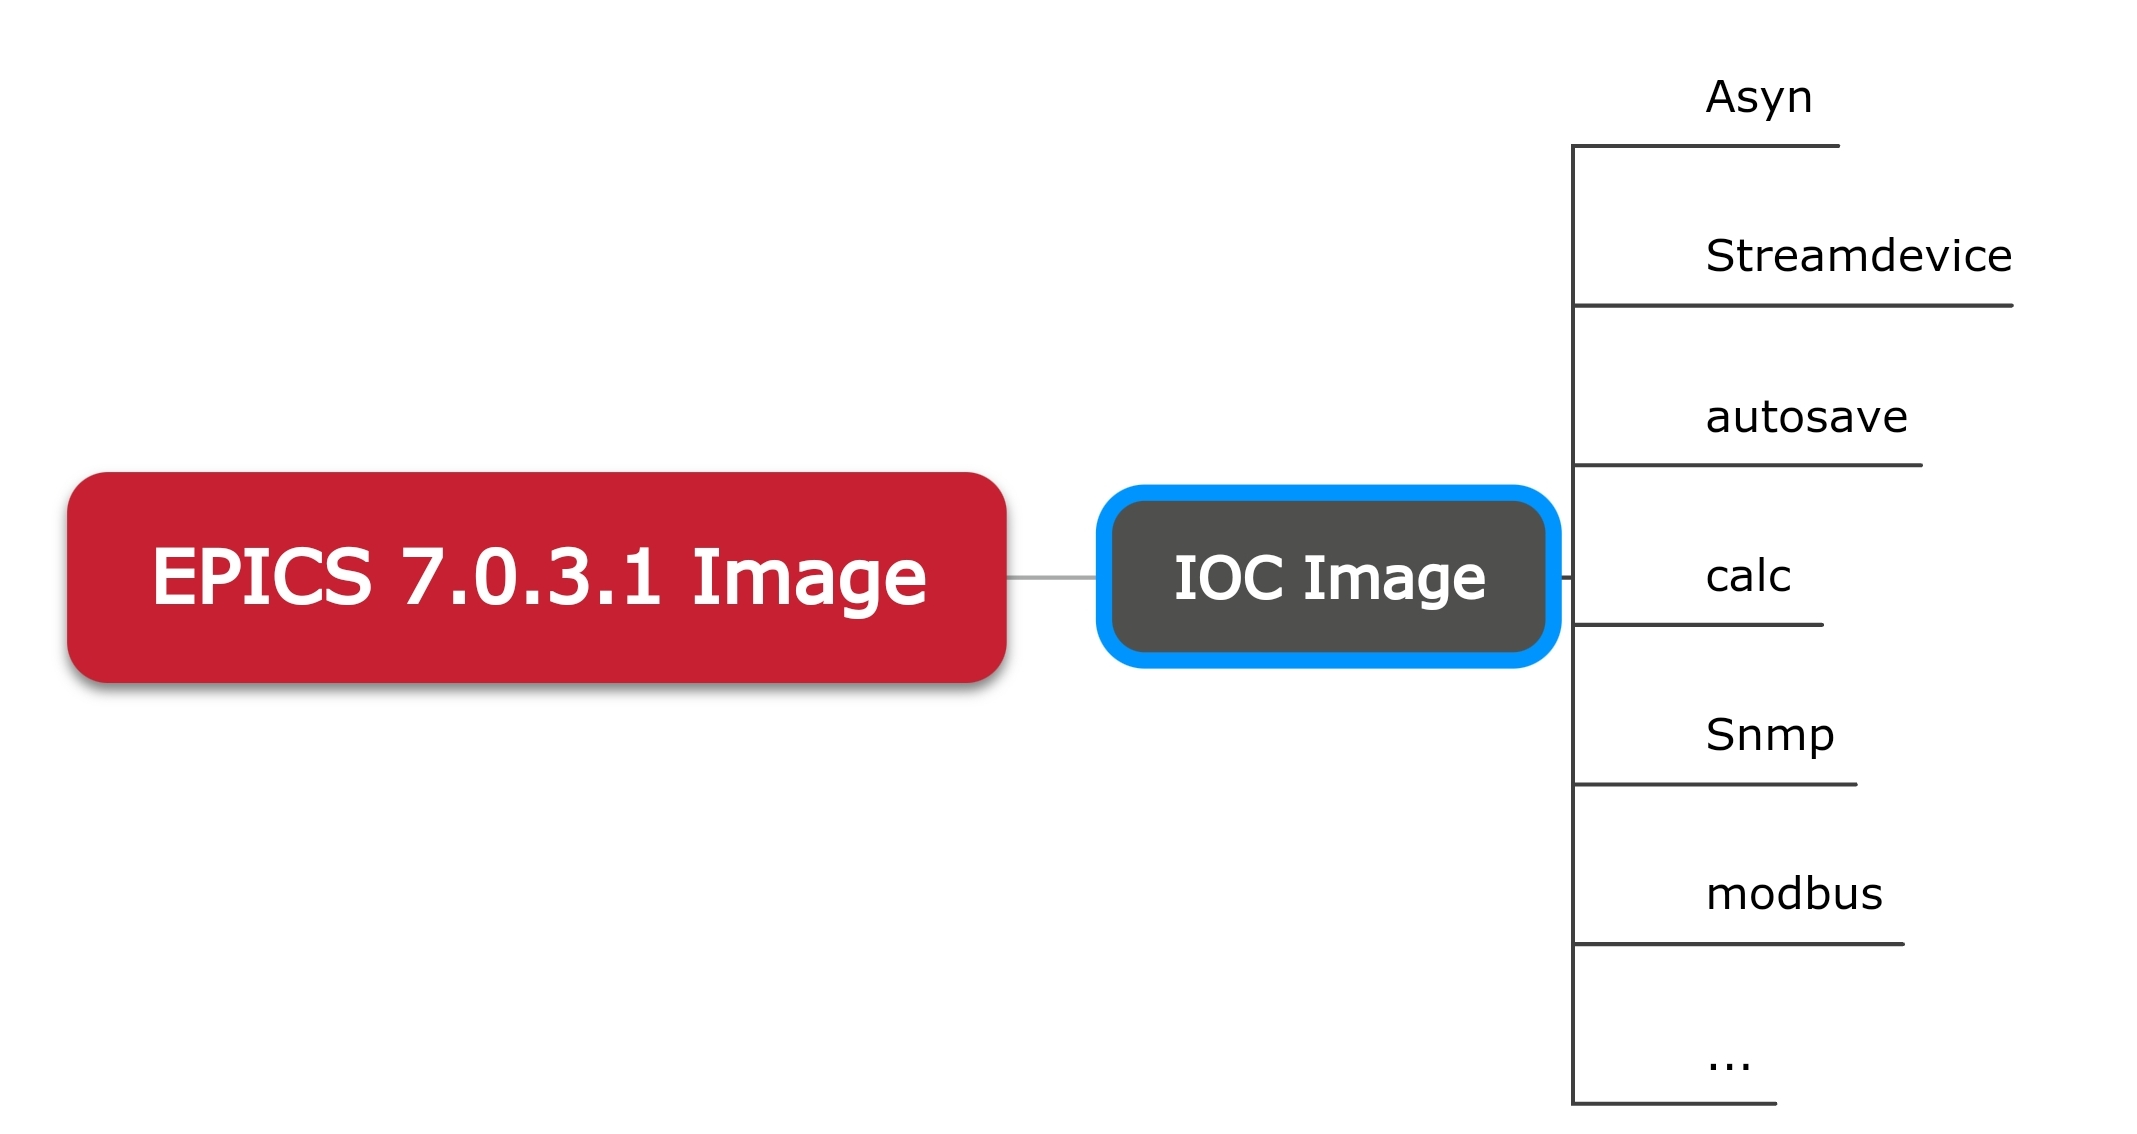
\includegraphics[width=0.7\columnwidth]{Chapter4/images/epics_ioc.jpg}
\caption{Schematic view of the EPICS 7.0.3.1 based \gls{IOC} image and the most commonly used modules.}
\label{fig_ioc1}
\end{figure}


A general idea of a containerized \gls{EPICS} \gls{IOC} is presented in Figure~\ref{fig_doc}. Every container is assigned an IP address for every Docker network it connects to. Each network has a default subnet mask and gateway. In order to connect the \gls{IOC} with other services, the ports used by \gls{EPICS} (5064, 5065 for channel access protocol and 7064, 7065 for PVAccess) need to be exposed.  The deployed containers use the host network to communicate with each other and other nodes.
\begin{figure}[!h]
\centering
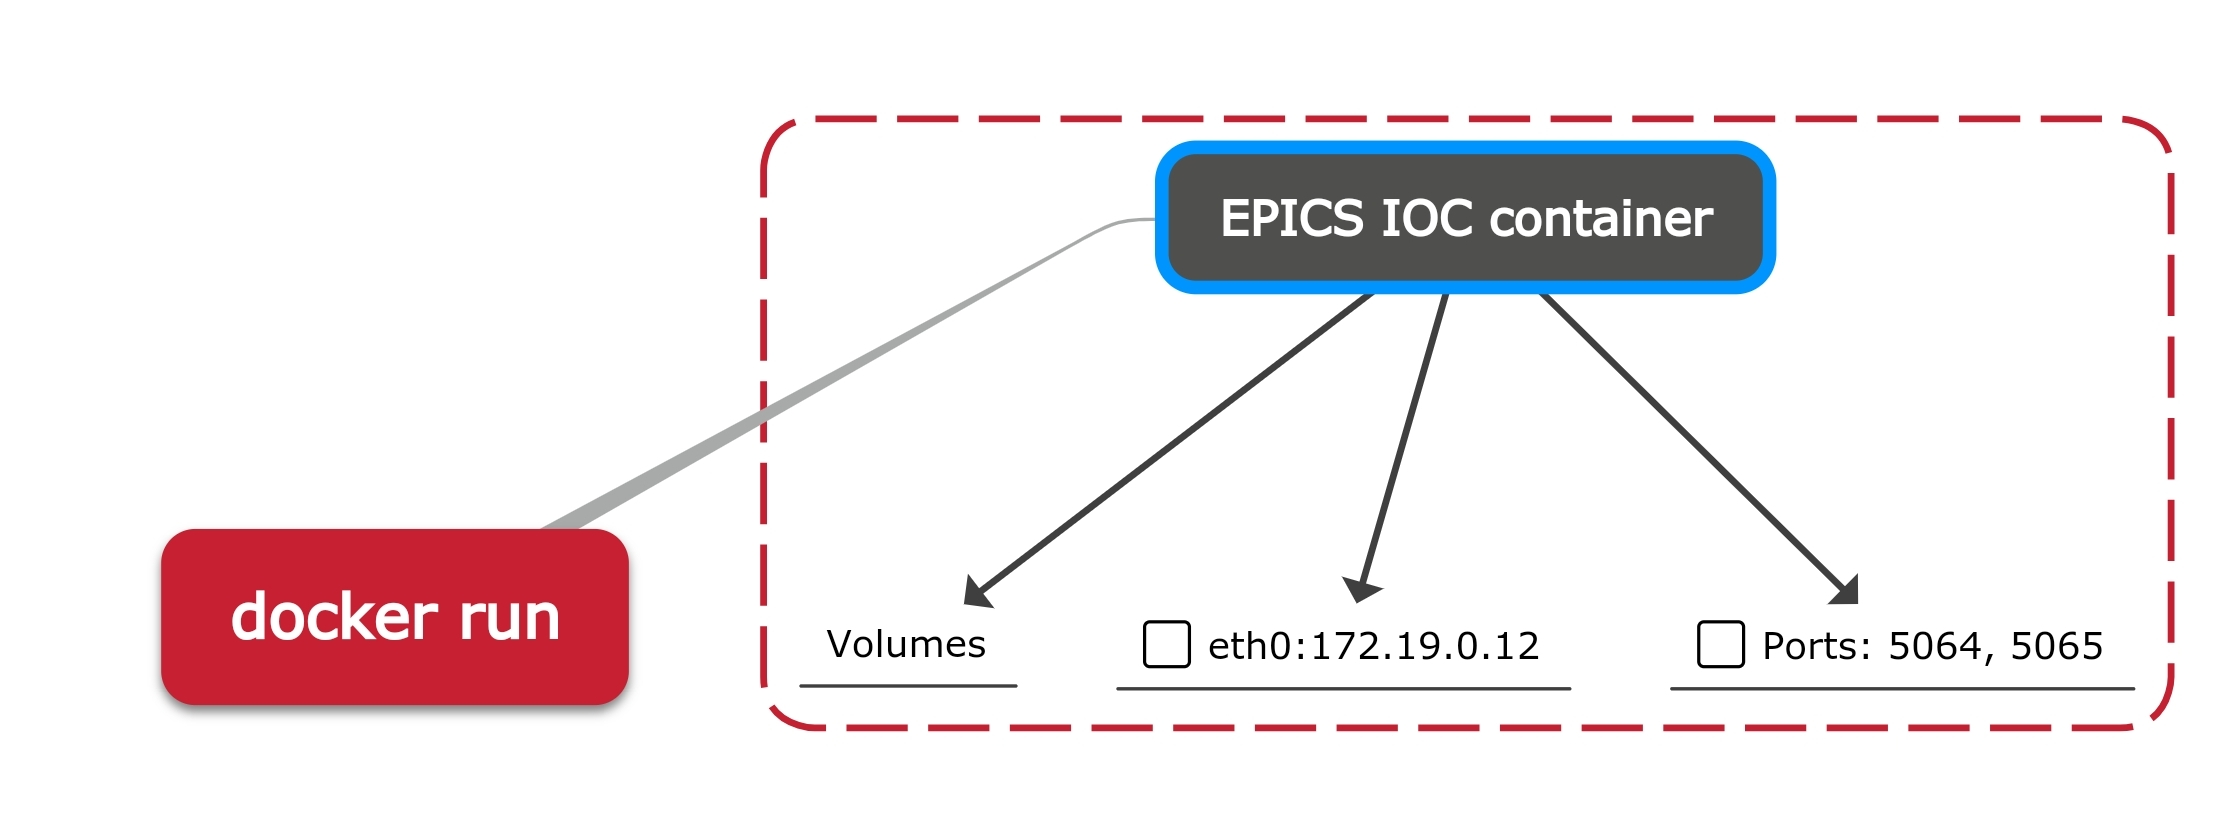
\includegraphics[width=0.75\columnwidth]{Chapter4/images/docker_run.jpg}
\caption{A general idea behind the containerization of an \gls{IOC}.}
\label{fig_doc}
\end{figure}
%\newpage
\section{Containerization platform -- Docker}
Docker was chosen as the platform to prepare the images and run the containers. There are also several alternatives to the docker engine, that allow running containers in rootless mode:
\begin{itemize}
    \item Podman~\cite{Podman} 
    \item Singularity~\cite{singularity}
\end{itemize}

For the use of containers in the final experiment, the following list of requirements must be taken into consideration:

\begin{itemize}
    \item Services should be accessible only by experts, crucial services should be hidden from operators (authorization).
    \item Ssh accesses to the DCS nodes should be limited by authorization plugins to avoid overloading,
    \item Experiment network should be segmented based on the goals and communication between software entities clearly, defined (\gls{DCS}, \gls{SCA}).
    \item Proper security context should exist for all the services (e.g., root privileges).
    \item All the changes in the cluster need to be logged.
    \item Unwanted kernel modules can't be loaded by the containers.
    \item Cluster and container should be redundant.
\end{itemize}


One of the features of Docker has been considered risky for the operation of the detector or experiment, especially considering the final system. Docker-based containers run with the root privileges, therefore posing a threat to the operation of the control system. The daemon is a part of the engine that runs the containers that have full privileges not only within the container but also on the node. If a container gets compromised, it may lead to potentially disastrous scenarios, including loss of data or potential threat to the detector -- e.g., killing the container. A compromised node can also endanger other nodes in the network.  Since late $2020$ it is possible to run Docker daemon and containers as a non-root user. Docker daemon and containers themselves can run inside a user namespace~\cite{docker_limitations}, therefore mitigating the risk.
%\begin{figure}[!h]
%\centering
%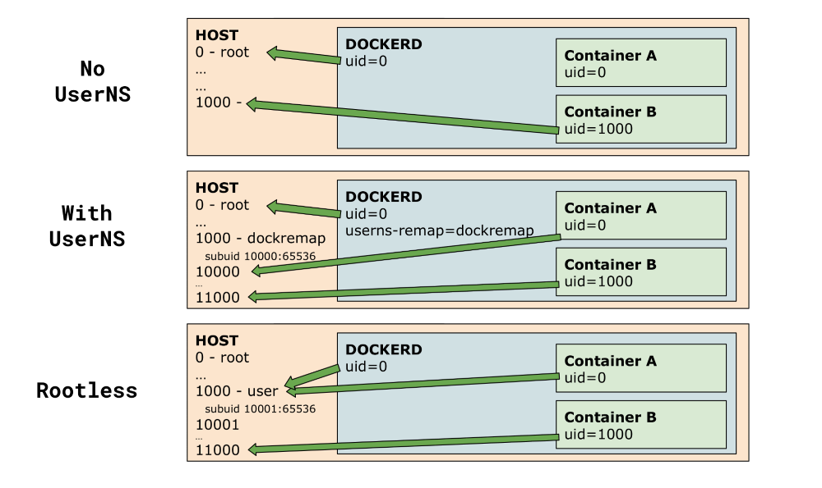
\includegraphics[width=0.8\columnwidth]{sections/images/docker.png}
%\caption{Rootless operation of the container}
%\label{fig_rootless}
%\end{figure}
 Thanks to the Open Container Initiative that defines container formats and runtimes, using different engines does not require many changes in the container image. 


\section{Multi-container applications}
Over the years \gls{EPICS} has become a framework that offers users many off-the-shelf applications that ease the implementation and configuration of a control system. Figure \ref{fig_dcs_node_msts} shows the most commonly used control-related applications. 

All the applications in figure~\ref{fig_dcs_node_msts} applications were used as containers based on prepared images and linked using Docker-compose, which is a tool for defining and running multi-container Docker applications~\cite{docker_compose}. To configure the containers a YAML\footnote{YAML is a human-friendly data serialization language for all programming languages~\cite{YAML}.} file has to be populated with the services settings (in this case the services refer to the applications, e.g., \gls{IOC}. This section summarizes the most important applications used for the \gls{DCS} and their functionalities.


\begin{figure}[!h]
\centering
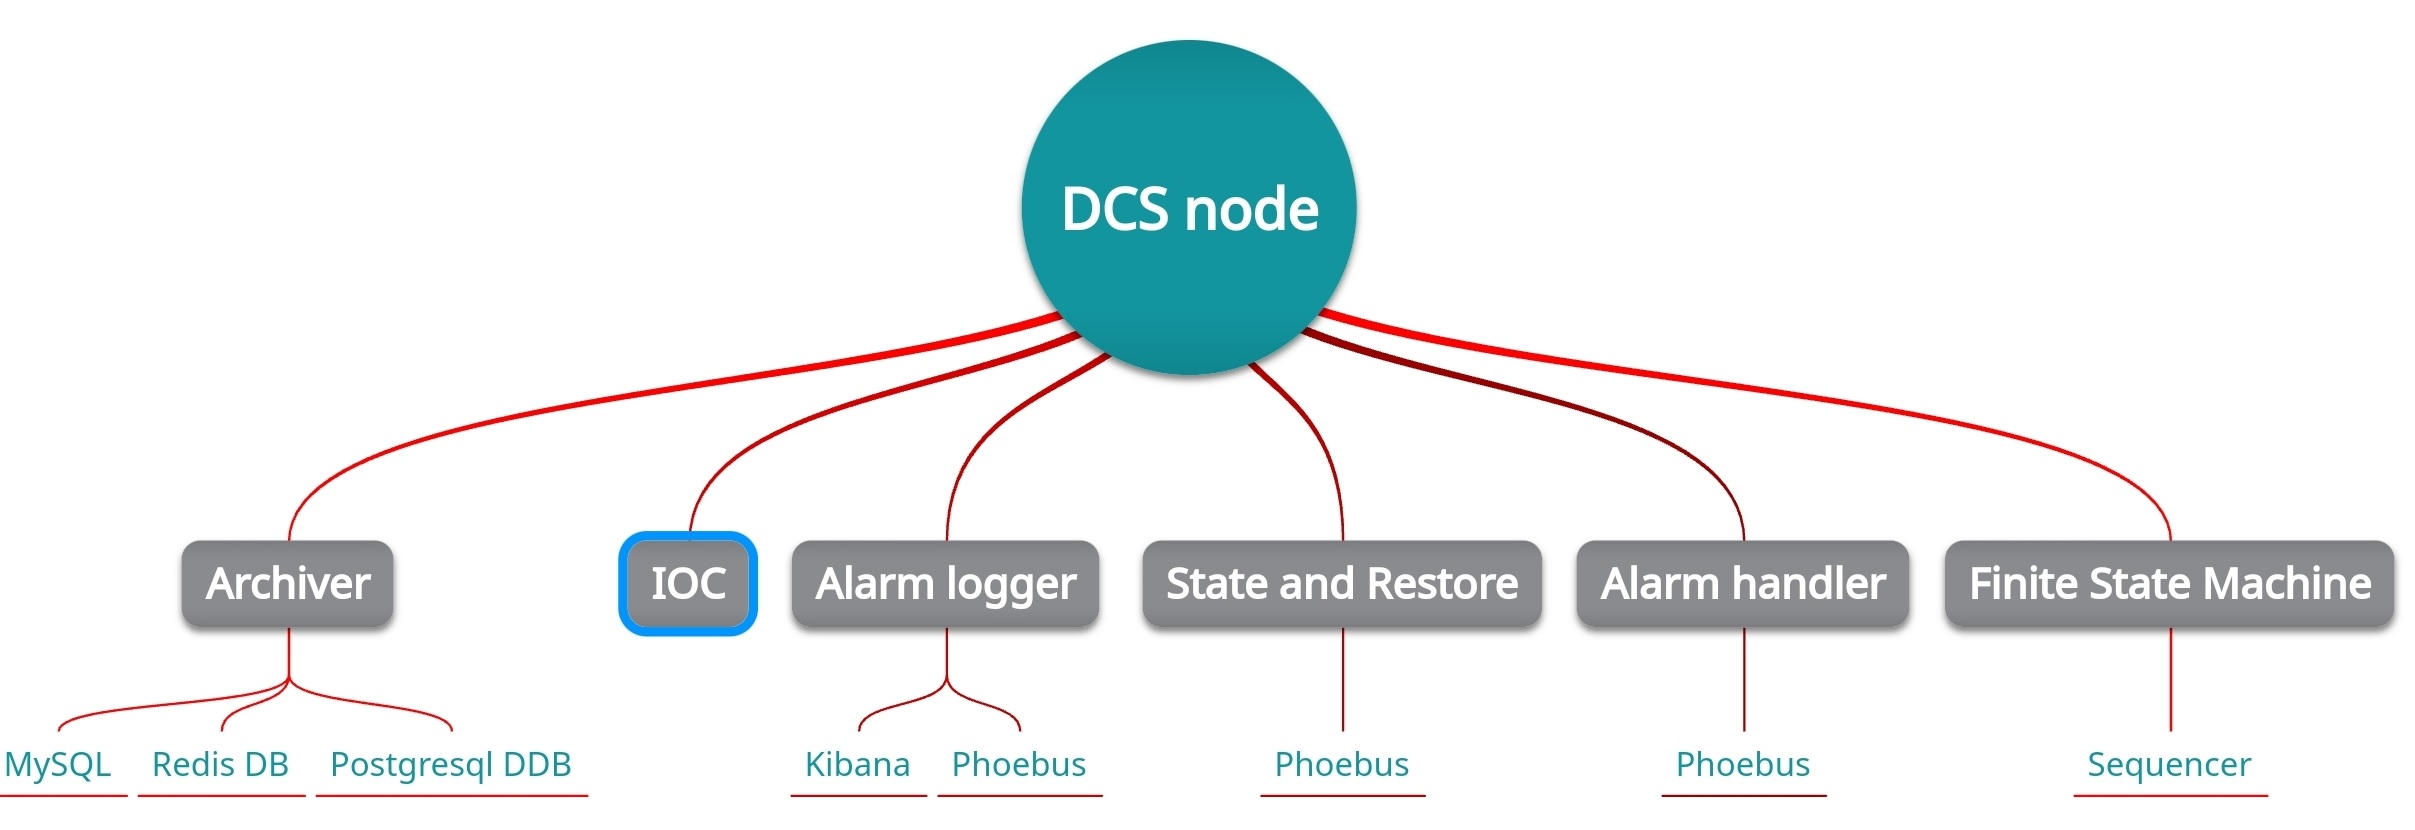
\includegraphics[width=0.95\columnwidth]{Chapter4/images/dcs_node.jpg}
\caption{Services used in addition to Phoebus functionalities, together forming a full-blown control system.}
\label{fig_dcs_node_msts}
\end{figure}
\newpage
\subsection{Control System Studio and Phoebus}

Control System Studio (\gls{CSS}) consists of open-source Java applications and modules which can be used in constructing a control system. Phoebus is an update to the \gls{CSS}, and significantly improves its performance by removing dependencies on Eclipse RCP. Phoebus uses both channel access protocol and \gls{PV} access, and it offers graphically based applications to access \gls{EPICS} \glspl{PV}, \glspl{OPI}, PVs history, etc. An example of a chiller \gls{GUI} is depicted in figure~\ref{fig_lauda1}. One of the main features of Phoebus is its modular nature. Users can develop and add their products, or just include or exclude applications or configurations. 


\begin{figure}[!h]
\centering
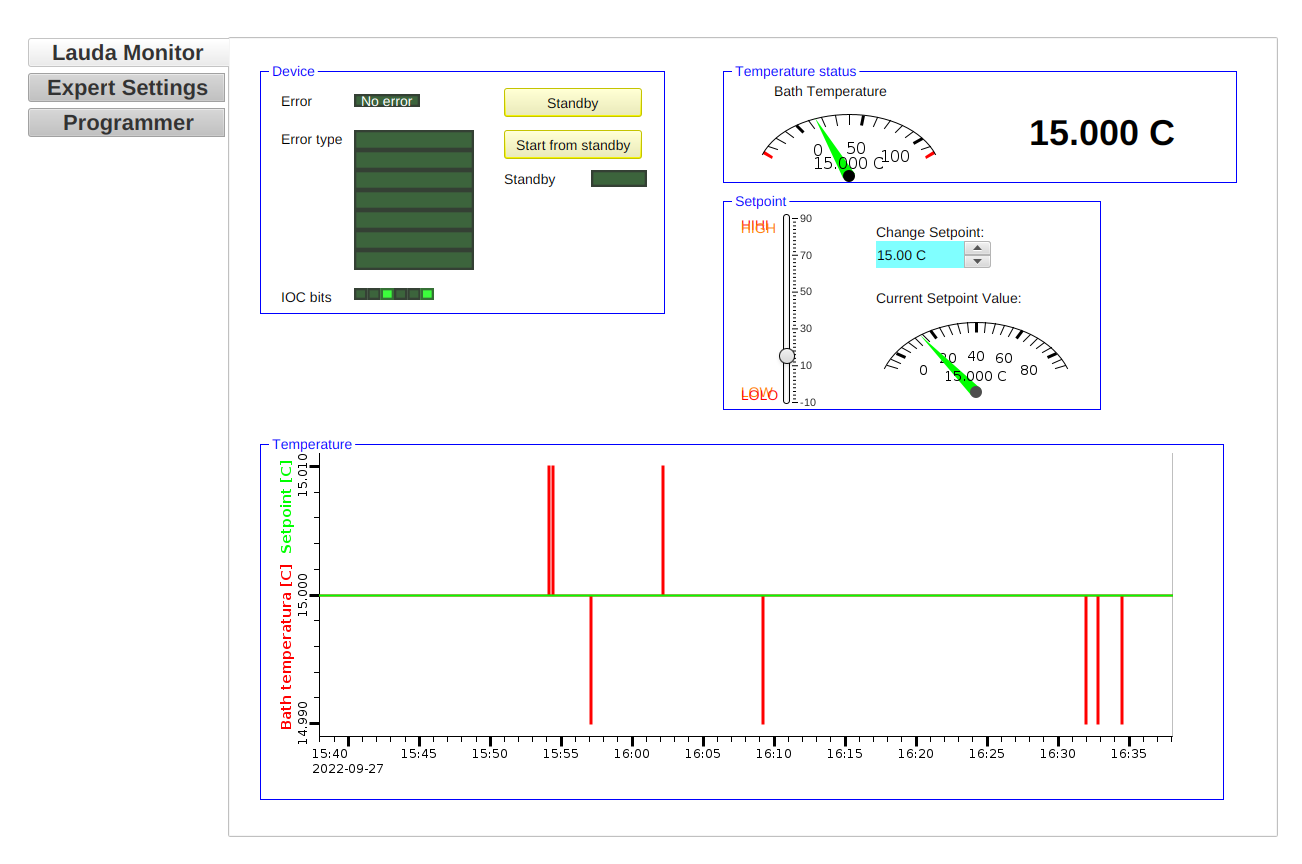
\includegraphics[width=1\columnwidth]{Chapter4/images/lauda1.png}
\caption{An example of a detector system \gls{GUI} for a cooling unit.}
\label{fig_lauda1}
\end{figure}

\newpage
\subsection{Solutions for archiving the data} \label{archiver}
An Archiver serves as one of the main building blocks of the \gls{DCS}, as it allows not only to look up the history of a given record, but also to download and post-process the data. Archivers make use of the publish/subscribe logic, updating the values on change. In general, the archiver must run smoothly, without significant downtime, and the linked database and other clients should also have a stable connection. A primary choice for \gls{STS} is the so-called Archiver Appliance~\cite{archiver_appliance}. An example of the archiver appliance is divided into short-term storage, medium-term storage, and long-term storage. In principle, a system administrator can adjust these settings to the needs of the specific case. The  four Tomcat containers\footnote{An Open source web server by the Apache foundation} are employed to handle the tasks of the archiver.  
%\begin{figure}[!h]
%\centering
%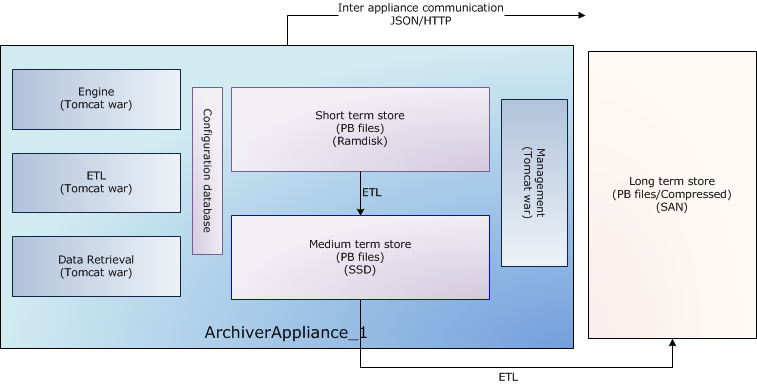
\includegraphics[width=0.7\columnwidth]{Chapter4/images/applarch.png}
%\caption{Architecture of a single appliance \cite{archiver_appliance}}
%\label{fig_archiver}
%\end{figure}
%\newline

The main advantage of the archiver include: 

\begin{itemize}
    \item Data retrieval can be integrated into Phoebus or Matlab.
    \item Wide range of supported formats.
    \item Stable performance, even with a hundred thousand \glspl{PV}.
\end{itemize}

Apart from the Archiver appliance, there are also alternative solutions:

\begin{itemize}
    \item Cassandra \cite{cassandra_archive},
    \item RDB Archive engine \cite{rdb_archive}.
\end{itemize}

\subsection{Alert communication with alarm server}
An alarm server monitors a chosen set of \glspl{PV}, including their alarm state. \gls{EPICS} records facilitate fields related to the alarm thresholds and their severity, evaluated each time the record is processed. Every numeric value could have two uppers and two lower boundaries, with assigned severities (NO\_ALARM, MINOR, MAJOR). \gls{EPICS} by itself, doesn't take any actions on the detector's hardware when the alarm threshold is exceeded. On the other hand, a Phoebus-based \gls{GUI} will change the font color (MINOR - orange, MAJOR - red) of the variable once the alarm appears. If the connection to the alarm server exists, then the server acts upon a change in the alarm status of a record. The user interfaces show alarms, allow acknowledgment, and provide guidance and helpful links. Apache Kafka is a distributed event store and stream-processing platform which serves as a communication bus between the alarm server and Phoebus. An example of the \gls{mSTS}'s alarm handling \gls{GUI} is depicted in Figure~\ref{fig_alarm1}. It provides not only a visual notification of an alarm but also guidance, displays, and commands.
\begin{figure}[!h]
\centering
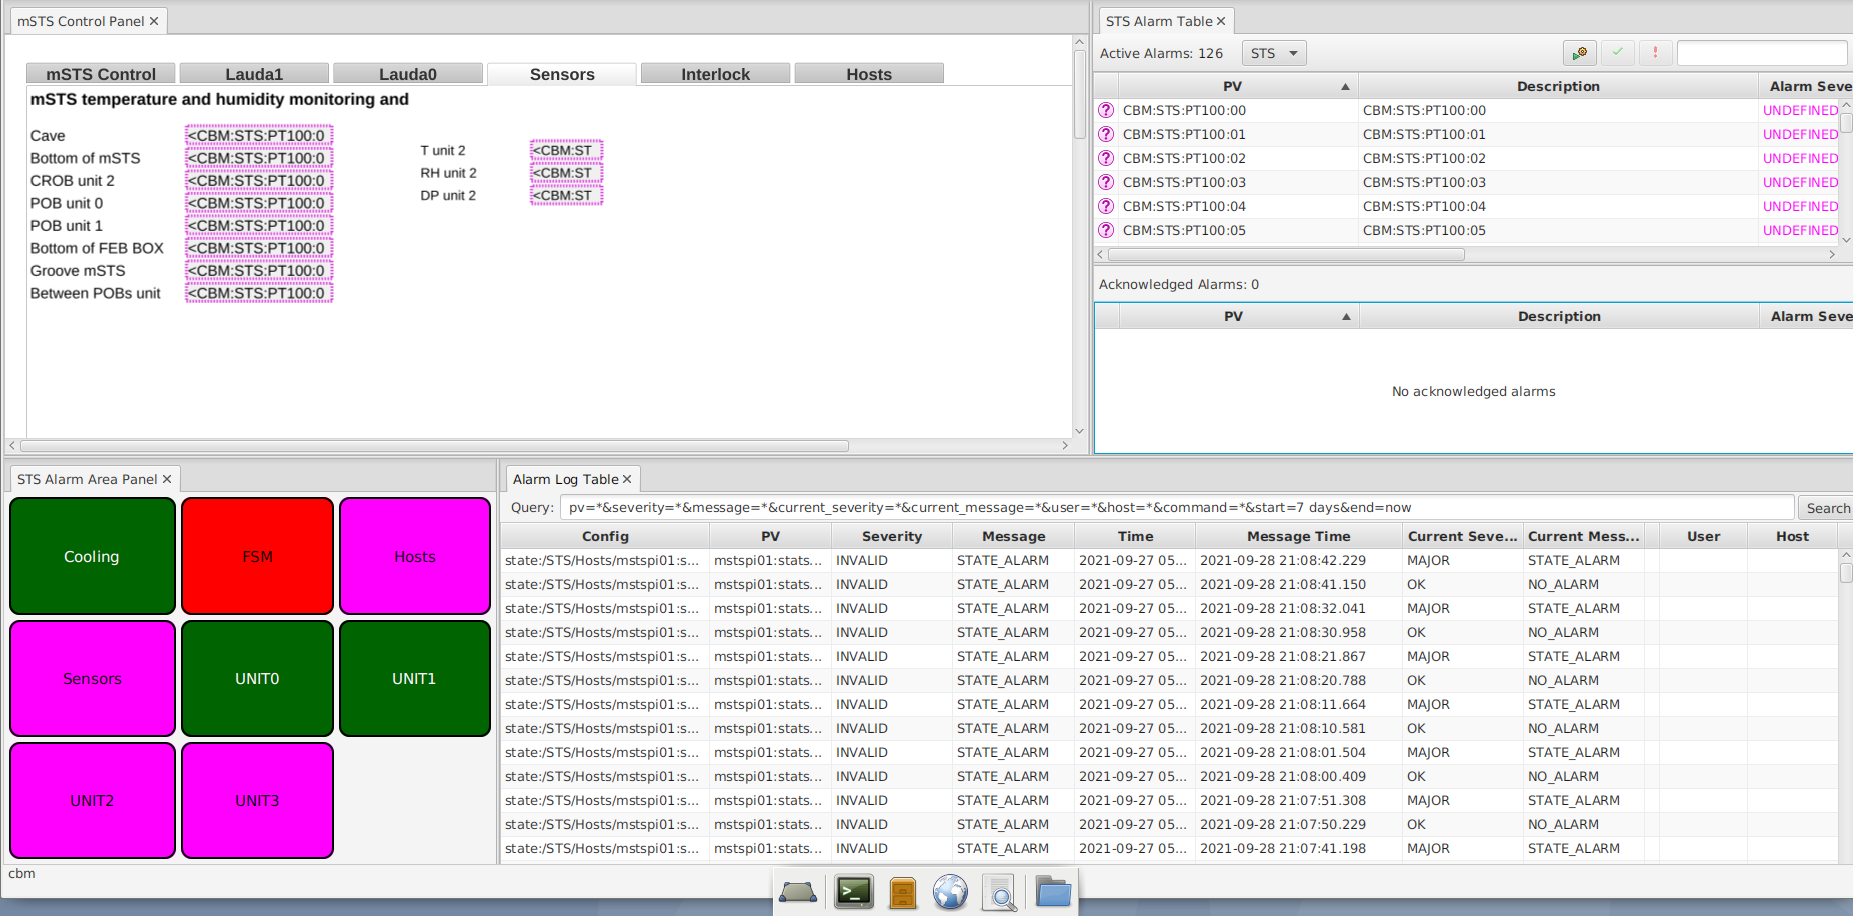
\includegraphics[width=1\columnwidth]{Chapter4/images/alarms.png}
\caption{Phoebus alarm handler view -  top left part some \gls{GUI}s, the top right part is the alarm table showing the current and acknowledged alarms, bottom left features a color status of respective nodes (e.g., cooling), bottom right shows the latest entries in the log.}
\label{fig_alarm1}
\end{figure}
\newpage
\subsection{State and commands logging}
Logging is another important part of the \gls{DCS}. It allows monitoring and checking of all the changes in the configuration and alarms of all the process variables. Thanks to the logs acquired by the dedicated service, debugging becomes much easier. The alarm logging service enables the logging of: configuration changes, state changes logging, and commands. Similarly to the alarm server, it uses Apache Kafka for data transfer. Apart from the logs, there is also a \gls{GUI} available in the Phoebus \cite{alarm_logger}, an operator can also use the Kibana\footnote{source-available data visualization software} web interface to discover patterns and trends in the data. 

\subsection{Finite state machine as an automation and safety mechanism}
A finite state machine (\gls{FSM}) is a construct that defines states and transitions between these states. In a given moment it has a clearly defined state and a given set of rules and conditions apply to this state. An input issued by an operator or automatically by a sensor(s) could trigger a transition. All transitions are unidirectional, but it's possible to define two opposite transitions, e.g., entering and escaping the error state. 
\newpage
One of the possibilities to implement a \gls{FSM} is to use Sequencer, which is a State Notation Language based on C/C++. 
\begin{itemize}
    \item start-up, shut-down, fault recovery, etc.,
    \item little C code, many states, many transitions,
    \item short compilation time, and can call any C++ code, easy connection to channelAccess.
\end{itemize}

One of the alternatives to the Sequencer and State Notation language is the PyEPICS-based library Pysmlib\cite{pysmlib}. It features several interesting functions like integrated watchdog logic, multi-threading, or configurable logging systems.


\section{Containerized EPICS-based framework}

The containers-based framework introduced in this chapter is the baseline for all the research and development activities throughout this thesis. In principle, most small and/or laboratory-based experimental setups don't require full-blown control systems. Hence, in the next two chapters two smaller framework applications will be introduced. In addition to that, the studies and their implications are discussed in detail. Chapter 6 is dedicated to the application of the full control system to the Phase-0 version of the \gls{STS}.
\chapter{Front-end electronics: monitoring, powering and its limitations}
\label{chap:containers}

\section{Monitoring of the Front End Electronics}

\gls{FEE} monitoring plays a crucial role in the detector operation, but also during the testing phase. Internal parameters of the \glspl{ASIC} in the \gls{ROB} or \gls{FEB} deliver information about the stability and onset of failure.


The first application of the introduced control framework was to read out several parameters from different readout chains (see section \ref{readout} for a detailed explanation of different readout chains). The \gls{ROB} and \gls{DPB} based readout chain were used to evaluate the possibility of interfacing the values from the \gls{DAQ} chain to the slow control and \gls{EPICS} based system.

The purpose was to monitor the stability of the readouts throughout different tests, e.g. during the thermal cycling of \gls{FEE}. A similar interface was also developed for the GBTemu readout chain. 

Two \glspl{FEB} - 16 STS-XYTERs were used to evaluate the performance of the interface and the ASICs. It constitutes in total 112 process variables, which makes it a relatively small setup. Those values were then stored in a database and are available from Phoebus for further analysis and visualization.

To get the values from the \glspl{ASIC} a soft \gls{IOC} with a pyEPICS~\cite{pyEPICS} interface was used. The monitoring studies included the registers and corresponding values available from \gls{GBT} \gls{SCA2} \gls{ASIC} \cite{GBT_SCA_ASIC} and three GBTX chips: 
\begin{itemize}
    \item GBT SCA - RSSI (Received Single Strength Indicator), input voltage $V_{in}$, 1.5~V DC/DC converter output voltage $V_{out}$, 2.5~V DC/DC converter output voltage $V_{out}$ (see figure~\ref{fig:ROB}), two temperature sensors,
    \item GBTX \gls{ASIC} - FEC (Forward Error Correction) counts.
\end{itemize}
%\newpage

\begin{figure}[!h]
    \centering
    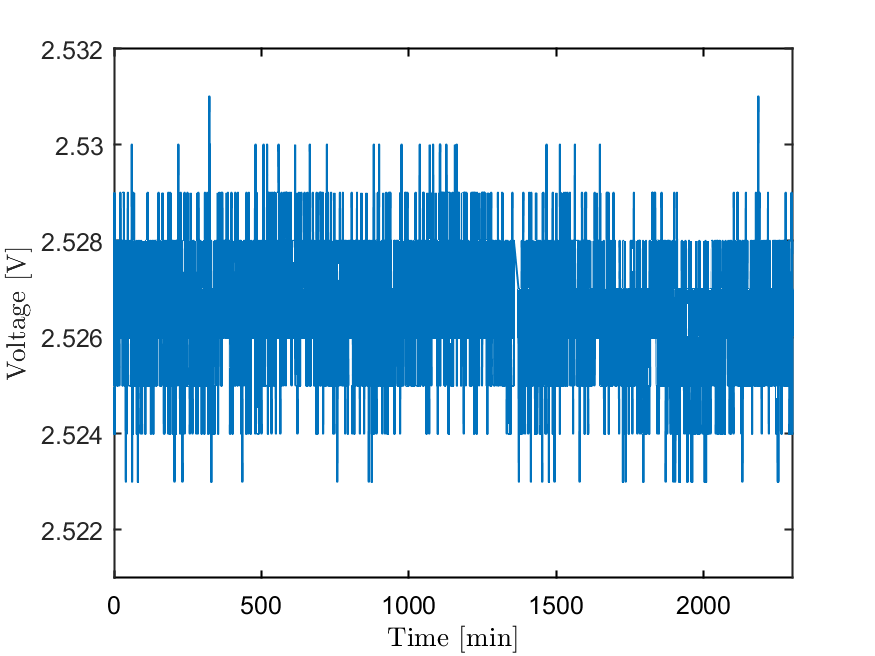
\includegraphics[width=0.65\columnwidth]{Chapter4/images/ROB.png}
    \caption{$V_{out}$ output voltage from one of the DC/DC converters in the \gls{ROB}}
    \label{fig:ROB}
\end{figure}

The STS-XYTER provides the following values - almost full counter, event missed counter, single event upset counter, the status register, and \gls{DAC} values: $V_{ddm}$, \gls{CSA} bias, temperature. 

\begin{figure}[!h]
    \centering
    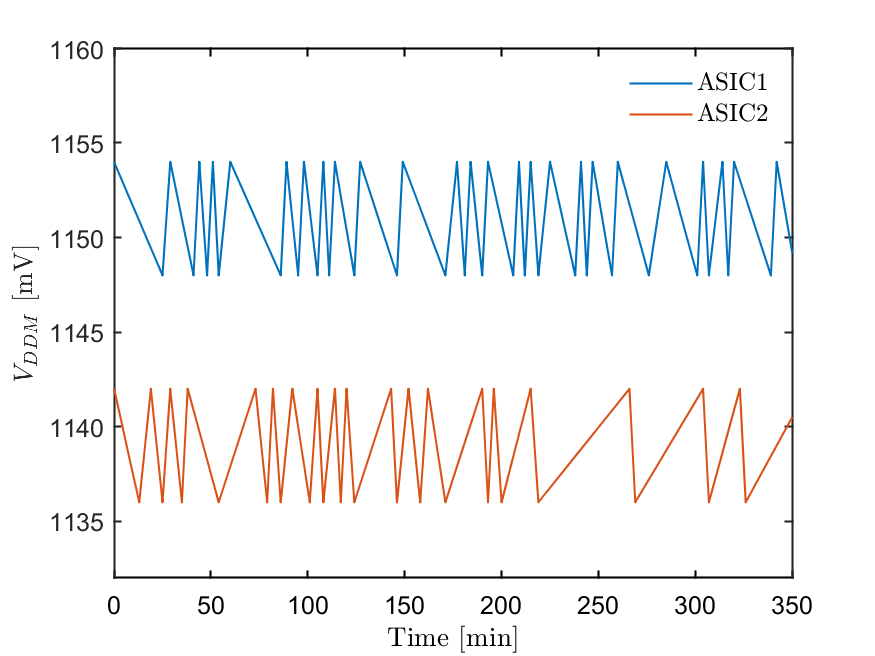
\includegraphics[width=0.65\columnwidth]{Chapter4/images/FEB.png}
    \caption{$V_{ddm}$ readouts from the diagnostic circuits of two ASICs}
    \label{fig:vddm_first}
\end{figure}

%\subsection{Parameters of the STS-XYTERv2 ASIC}
%\subsection{GBTX and GBT ASIC monitoring}
\newpage
\section{Irradiation studies of the powering units}
Radiation-induced effects in electronics play an important role in accelerator facilities, where different particle species may elevate radiation levels even in relatively remote areas. Depending on many factors, i.a. location of the setup, intensity or energy of the incident particles, damage caused to a semiconductor device may vary greatly. A particle could cause no observable effect, transient disruption of circuit operation, a change of logic state, or even permanent damage to the device or integrated circuit (IC)~\cite{dodd}. The detector will be powered by about 140 low voltage modules, providing 2100 power channels. In order to estimate the Single Event Effects (\gls{SEE}) in the powering electronics in the envisaged radiation environment, two irradiation campaigns took place in \gls{GSI}, Darmstadt.  The first one was conducted at the mini-CBM experiment and the second was realized next to the electrostatic septum of the SIS18 synchrotron. These irradiation campaigns aimed at detecting radiation-induced soft errors in the power units' electronics and estimating its rate.


\subsection{Single Event Effects in the electronics}
A variety of different elements and chemical compounds can be used in electronics, including silicon, silicon dioxide ($\mathrm{SiO}_{2}$), or boron. The high ambient flux of particles in a particle accelerator environment usually consists of charged particles (mostly protons, and electrons), high-energy photons (gamma and X-rays), and a broad spectrum of neutrons. Different interaction mechanisms may cause both stochastic and deterministic effects in electronics. These effects are directly related to the integrated dose and linear energy transfer (\gls{LET}) of the incident particles ~\cite{electronic_system_on_module}. Radiation-induced soft errors have become a huge concern in advanced computer chips because uncorrected, they produce a failure rate that is higher than all the other mechanisms compromising reliability combined~\cite{1545891}. Neutrons do not cause direct ionization in silicon or oxygen. These neutral particles interact elastically as well as inelastically, resulting either in the creation of other nuclei and the emission of a light particle or in changes in the kinetic energies of the participants. A few neutron threshold energies for reactions with oxygen and silicon are summarized in Table~\ref{cross-seciton}. The cross-section for neutron reactions generally decreases with the energy. Moreover, neutrons can indirectly cause \gls{SEE} by secondary radiation, for example, a reaction with boron which results in the emission of an $\alpha$ particle $^{10}\mathrm{B}(n,\alpha)^{7}\mathrm{Li}$~\cite{1545891,neutrons_energy,neutrons_energy_2}. 

\begin{table}[!h]
\centering
\caption{Threshold energies of neutron reactions with silicon and oxygen nuclei~\cite{ENDF}.}
\begin{tabular}{lc}
\hline
Reaction         & Neutron Threshold Energy (MeV) \\ \hline
Si elastic       & 0                              \\
Si(n,$\alpha$)   & 2.75                           \\
Si(n,p)          & 4                              \\
Si(n,d)          & 10.5                           \\
Si(n,$n-\alpha$) & 10.35                          \\ \hline
O elastic        & 0                              \\
O(n,$\alpha$)    & 2.35                           \\
O(n,$n-\alpha$)  & 7.61                           \\
O(n,p)           & 10.24                          \\
O(n,d)           & 10.53                         
\end{tabular}

\label{cross-seciton}
\end{table}

\newpage
\subsection{Motivation}

The powering of the Front End Boards (\gls{FEB}s), together with the data processing electronics, sum up to about 2100 low voltage channels, operated in about 140 low voltage modules, 16 channels each. All of them will be placed in a protected area within the cave with an elevated radiation level. The estimated dose values were calculated by A. Senger using FLUKA code (see Figure~\ref{fig:mCBM})~\cite{FLUKA}. 

\begin{figure}[!h]
    \centering
   % 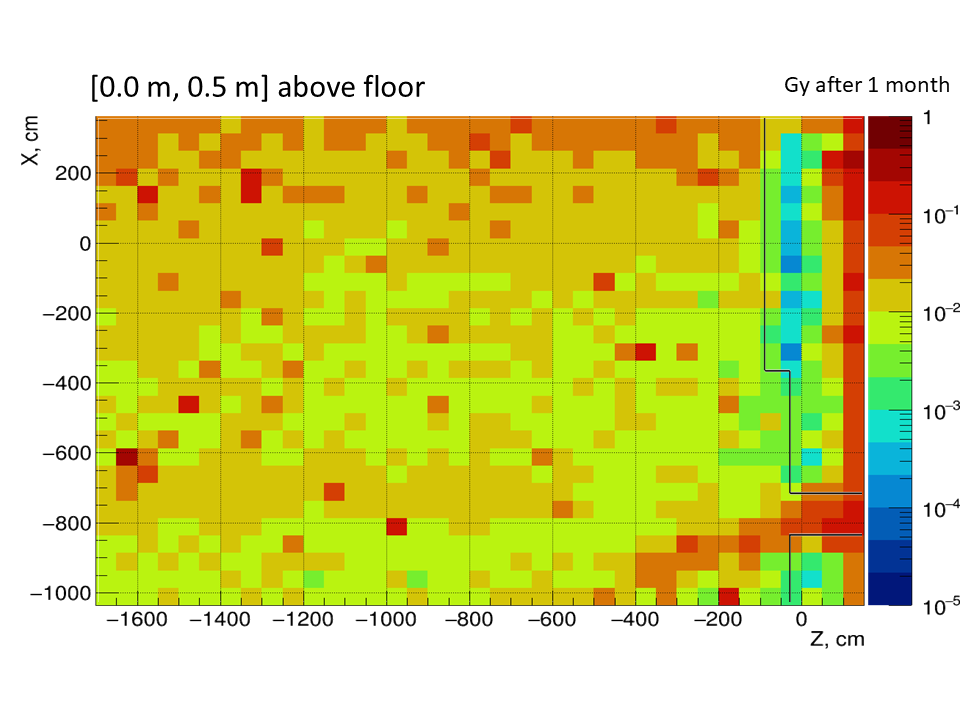
\includegraphics[width=0.95\columnwidth]{images/dose3.png}
    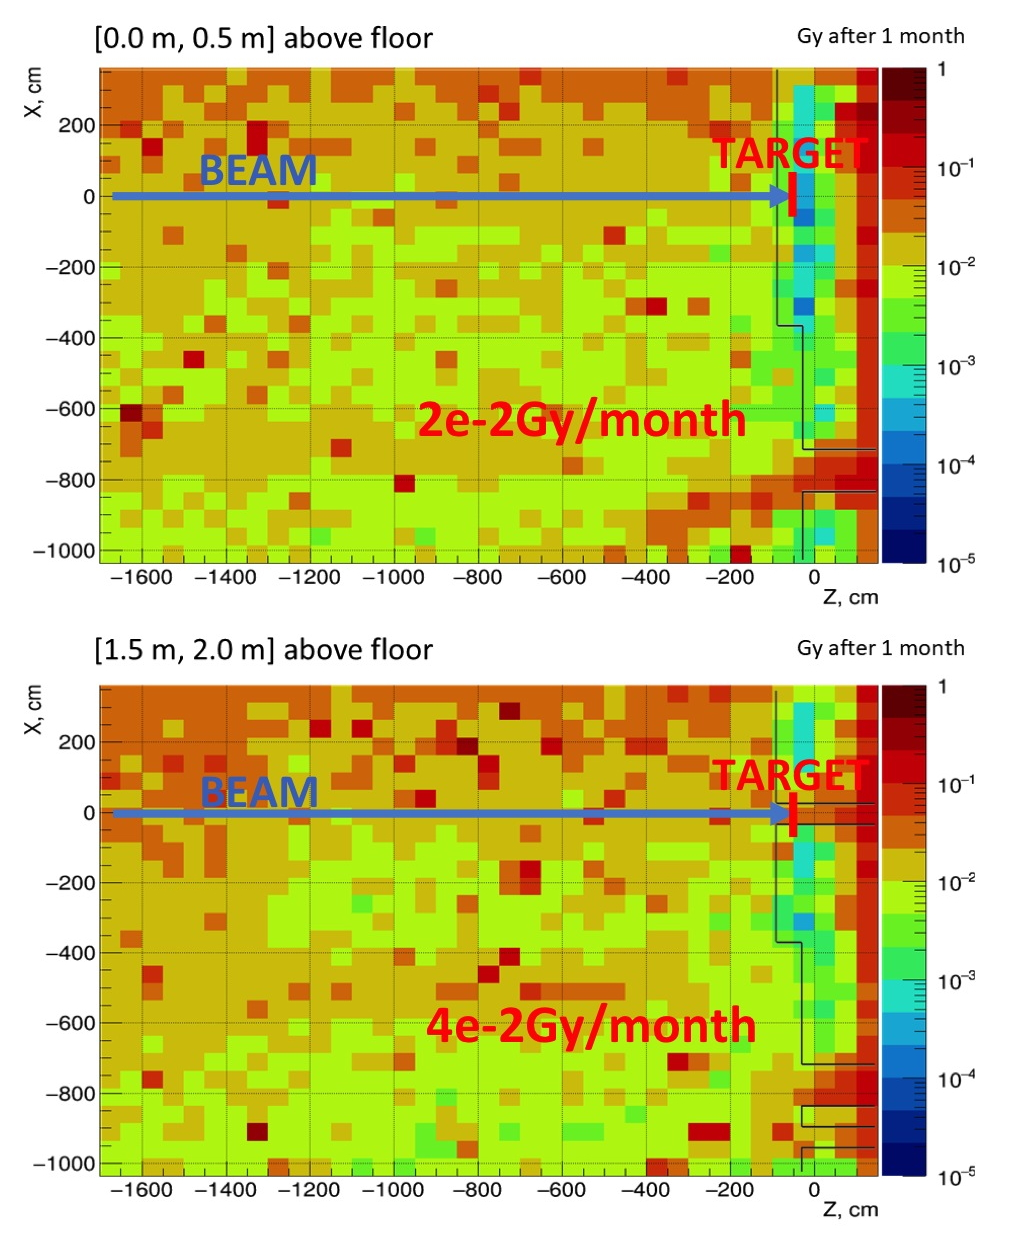
\includegraphics[width=0.55\columnwidth]{Chapter4/images/Dose00.jpg}
    \caption{Expected dose distribution in the air in the \gls{CBM}
cave under the platform in (11 AGeV Au $10^{9} \mathrm{\ ions/s}$ on 1\% Au
interaction target) 0 to 0.5 m and 1.5 m to 2 m above the ground} 
    \label{fig:mCBM}
\end{figure}
%\newpage
For the gold beam with the highest available intensities ($10^{9}\mathrm{\ ions/s}$) and energies (11~AGeV), we expect a total dose level of 20 \footnote{Gray is a SI unit of ionizing radiation dose, defined as the absorption of one joule of radiation energy per kilogram of matter \cite{gray}}{mGy} after 1 month of operation in the area between 0 and 0.5 m above the ground (at the planned location of the power crates x = -600 cm, z = -600 cm) and 40 mGy between 1.5 m and 2 m above the ground (x = -600 cm, z = -600 cm). A failure in the low voltage powering of the FEE may lead to a rapid decrease of temperature, as the primary coolant temperature may reach down to $-40^{\circ}\mathrm{C}$, consequently making the FEE susceptible to thermal stress. The effects of radiation must be therefore studied to ensure the safe operation of the \gls{STS}. Estimation of the soft error rate (\gls{SER}) may also indicate whether there is a need for further shielding of the power electronics in order to minimize the overall dose.

\newpage
\subsection{Methodology}
The subject of the irradiation campaign was a MPOD mini crate with one low voltage (WIENER) and one high voltage (ISEG) module. The crate's CC24 controller (ISEG) offers an embedded \gls{EPICS} Input Output controller, which was used to detect radiation-induced channel or module failures. All registered events were stored in a dedicated database.  In order to correlate the soft failure rate with the absorbed dose, two types of thermoluminescent dosimeters were used. A larger polyethylene sphere (d = 30 cm) was used to measure the neutron ambient dose, whilst the cylinder (d = 5 cm, h = 6 cm) measured other particles~\cite{bonner}. We assume that the conditions (neutron spectra - mostly thermal neutrons, neutron moderators, etc.) at the \gls{CBM} experiment will be similar to conditions at SIS18, and at the \gls{mCBM} experiment. Therefore, the quality factor, which takes into account both \gls{LET} and relative biological effectiveness (\gls{RBE}), to convert the measured given in Sv to absorbed energy in Gy is 5 for both irradiation campaigns. The dose measured with the cylinder is assumed to have a quality factor of 1.

\subsection{Poisson distribution}
We assume that failure events (radiation-induced errors) are statistically independent and are driven by purely stochastic factors. In addition to that, we take into account only the total dose measured by the dosimeters, thus rapid dose changes and their effect are not investigated in this contribution. In such a case, the probability of observing $n_{m}$ events with the mean value $\mu$ is described by the Poisson distribution:\newline
\begin{equation}
    p(n|\mu) = \frac{\mu^{n}}{n!}e^{-\mu}
\end{equation}
The total number of events is considered to be the average $\mu$, as this is the most reasonable assumption.
Assuming 68\% confidence levels for values $n_{m} > 2$ we can apply the following equations to estimate the distribution's bands (see Figure~\ref{fig:poisson})~\cite{schmidt}.
If in an experiment $\mu$ events are measured, we conclude that the standard deviation is described by $\mu - \sqrt{\mu}$ and $\mu + 1 + \mu$ around the average value $\mu$.
\begin{figure}[!h]
    \centering
    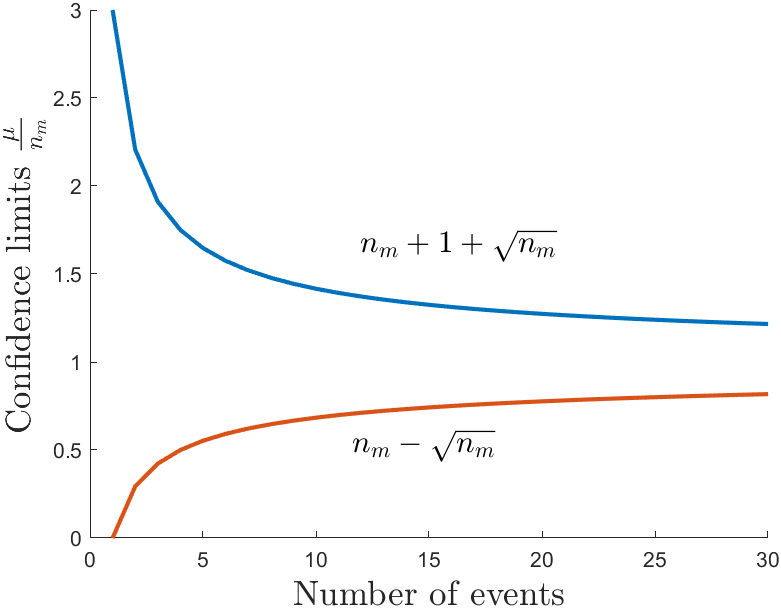
\includegraphics[width=0.55\columnwidth]{Chapter4/images/poisson.png}
    \caption{Estimated bands of the Poisson distribution~\cite{schmidt}}
    \label{fig:poisson}
\end{figure}
%\newpage
For $n_{m} \leq 2$ previously mentioned, estimations do not provide accurate results, therefore upper and lower bands need to be calculated explicitly. According to~\cite{schmidt}:



\begin{table}[!h]
\centering
\begin{tabular}{ccc}
\hline
Number of counts & \multicolumn{2}{c}{Poisonn's distrubution} \\ \cline{2-3} 
$n_{m}$          & $\mu_{l}$            & $\mu_{u}$           \\ \hline
0                & 0                    & 1.84                \\
1                & 0.173                & 3.30                \\
2                & 0.708                & 4.64                \\ \hline
\end{tabular}

\end{table}
\newpage
\subsection{Irradiation at the mCBM experiment}
In order to investigate electronics' operation under the realistic conditions, that low voltage modules will face during the CBM experiment, an irradiation campaign took place at the \gls{mCBM} experiment (see figure~\ref{fig:CBM1}). Different intensities and reaction systems (Au+Au, Au+Ni, etc.) were exercised during the experiment.
\begin{figure}[!h]
    \centering
    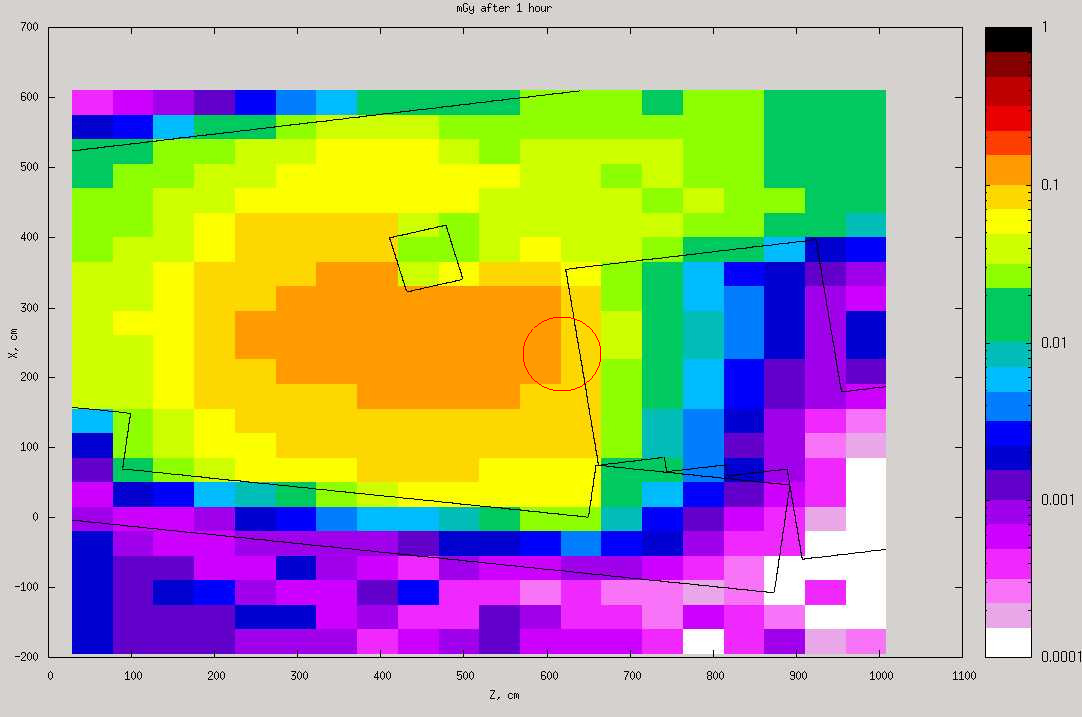
\includegraphics[width=0.65\columnwidth]{Chapter4/images/dose1.jpg}
    \caption{Expected dose rate distribution (mGy/hour) in the \gls{mCBM} cave with 2 AGeV O ions beam of $10^{7}\mathrm{\ ions/s}$ on 4 mm Ni target. In the encircled area the dose reached about 0.1~mG/hour}
     \label{fig:CBM1}
\end{figure}
\begin{figure}[!h]
    \centering
    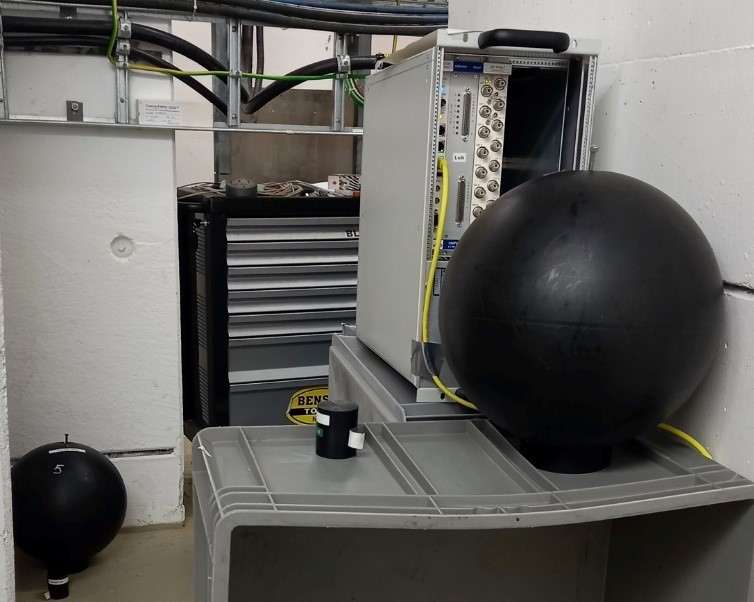
\includegraphics[width=0.5\columnwidth]{Chapter4/images/crate.jpg}
    \caption{Crate irradiation setup at the \gls{mCBM} experiment. The photo depicts two TLD dosimeters in the background, and two TLD dosimeters and the crate in the foreground}
    \label{fig:crate}
\end{figure}
\newpage
To measure the dose that the crate was exposed to, four thermoluminescent dosimeters (\gls{TLD}) with moderators were used (Figure~\ref{fig:crate}). Two TLDs placed far away from the crate served as a reference. During the irradiation at the \gls{mCBM} experiment, the dosimeters were read out twice, in order to evaluate the total dose received by the crate. The first value was $19.72\mathrm{\ mGy}$ and  the second one was $72.31\mathrm{\ mGy}$. 

A \gls{SEE} in the low voltage module occurred in each part of the irradiation. In both cases, it was possible to recover the functionalities by enabling the channels again. In total, $n=2$ after ($92\pm{4.6}\mathrm{\ mGy}$), considering standard 5\% uncertainty for the TLD. After applying lower and upper limits we find:
%\newpage
In total, $n=2$ after ($92\pm{4.6}\mathrm{\ mGy}$).
After applying lower and upper limits we get:
\begin{equation}
    D_{lower}=\frac{92}{0.708} = 129.9\mathrm{\ mGy}
\end{equation}
\begin{equation}
    D_{upper}=\frac{92}{4.64} = 19.8\mathrm{\ mGy}
\end{equation}
The uncertainty for $n_{m}=2$ is extremely high and equals to $\mathrm{46}_{-26}^{+84}$ mGy, therefore no clear conclusion on the behavior of the crate could be made. To further increase the statistics, a second irradiation campaign took place at the electrostatic septum of the SIS18 synchrotron. 
%\vspace{10cm}
\subsection{Irradiation at the SIS18 septum}
\subsubsection{Setup}
The setup at the SIS18's septum consisted of two \gls{TLD} dosimeters (for neutrons and other particles separately). Furthermore, the total doses from TLDs were supplemented with readouts from two active dosimeters placed behind the wall (see Figure~\ref{fig:spec_des}). 
\begin{figure}[!ht]
    \centering
    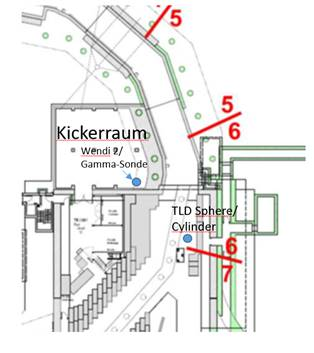
\includegraphics[width=0.45\columnwidth]{Chapter4/images/septum.jpg}
    \caption{Location of the dosimeters and crate at the SIS18. The so-called Kickerraum contained WENDI-2 and Gamma probe, whereas two TLD dosimeters were placed next to the power crate - depicted with a blue dot between segments 6 and 7.}
    \label{fig:spec_des}
\end{figure}

Wendi-2 is a precise wide-energy neutron dosimeter~\cite{wendi} that was used to determine the neutron dose rate in the so-called Kickerraum. Due to the shielding of the wall, the gamma probe measured mostly background radiation. The MPOD mini crate was placed next to the TLD dosimeters. In order to calculate the active neutron dose next to the crate, a ratio of total doses from both measurement places was used. 
\newpage
\subsubsection{Results}
During the irradiation period, readings from the dosimeters reached $106.1\mathrm{\ mSv}$ and \\$27.7\mathrm{\ mSv}$ for neutrons and other particles respectively.
%(Figure~\ref{fig:spectrum} depicts neutrons spectrum at the irradiation place).
%\begin{figure}[!ht]
%    \centering
%    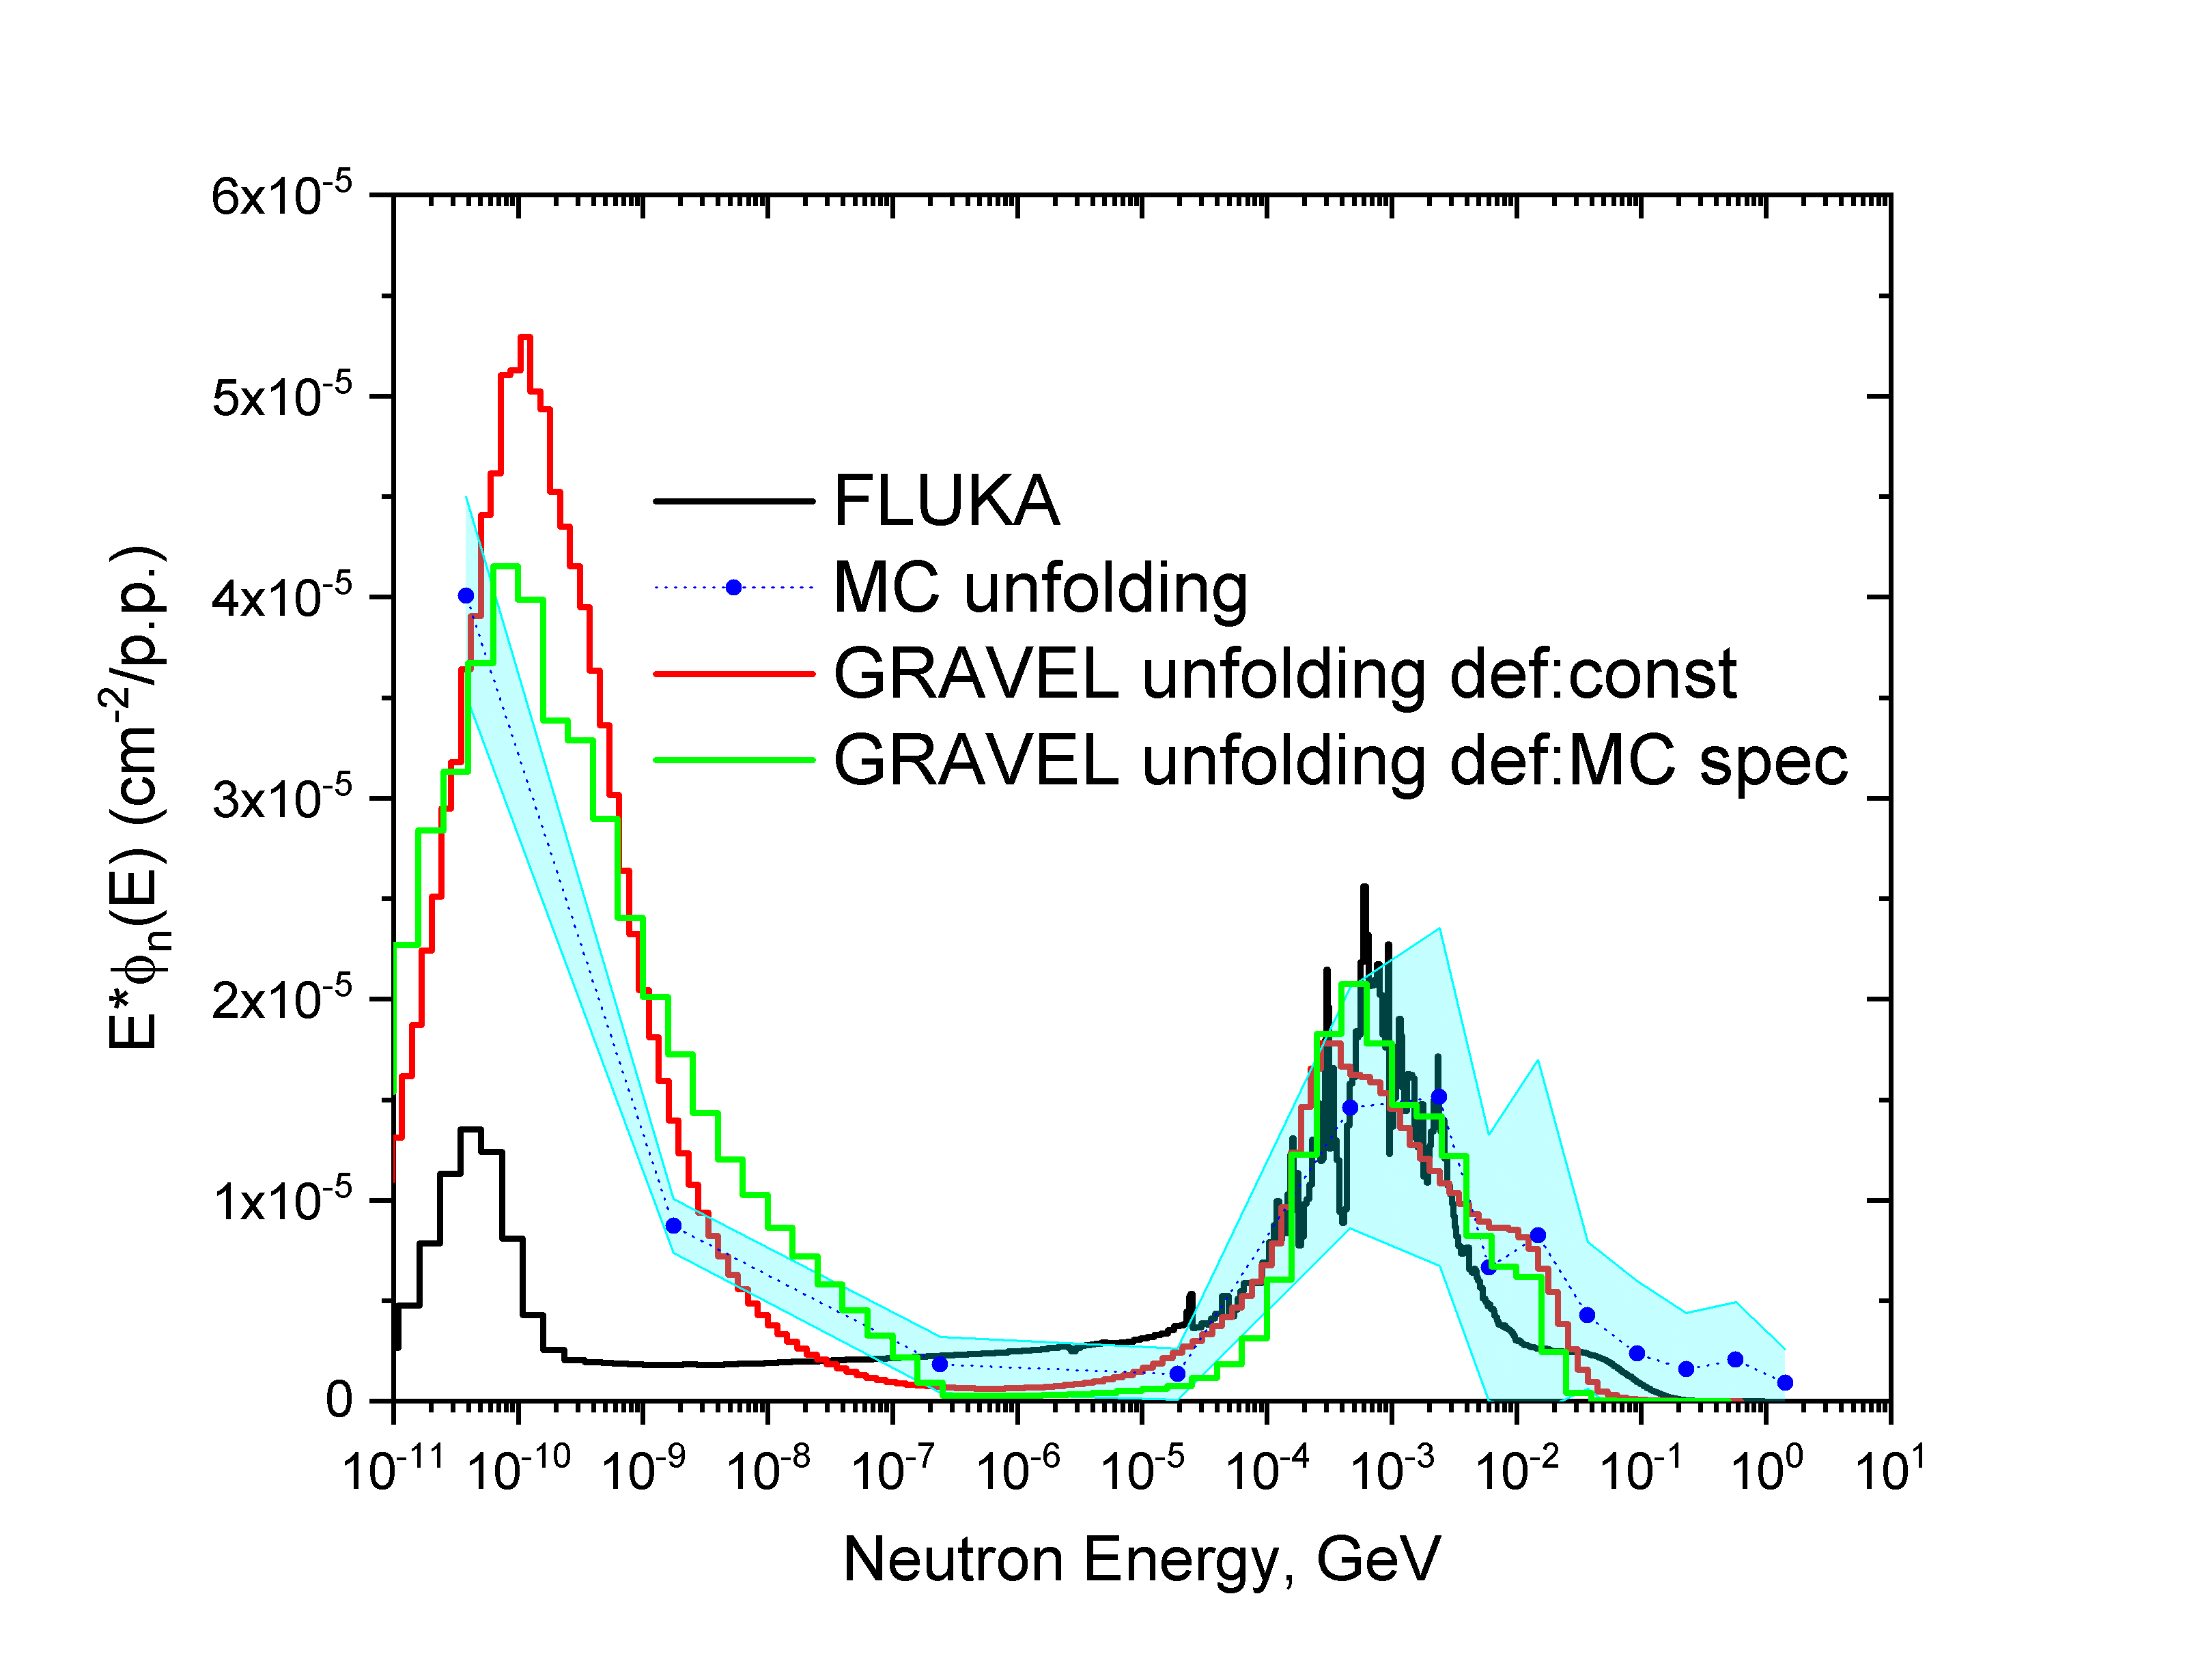
\includegraphics[width=0.9\columnwidth]{Chapter4/images/fig5.png}
%    \caption{Neutron spectrum at the measurement location (SIS18 septum). It is based on the measurement of argon ions at 550 MeV/u. The first peak is related to the thermal neutrons and %the second one to the fast neutrons}
%    \label{fig:spectrum}
%\end{figure}
Using assumed quality factors, we convert the ambient dose to the absorbed dose values. Hence, we get in total $49\pm{2}\mathrm{\ mGy}$, taking into account 5\% standard uncertainty of the TLD dosimeters. During the irradiation 11, radiation-induced soft failures were identified in the low voltage module. Therefore, we can estimate an average dose after which a low voltage failure might take place.
\begin{figure}[!h]
    \centering
    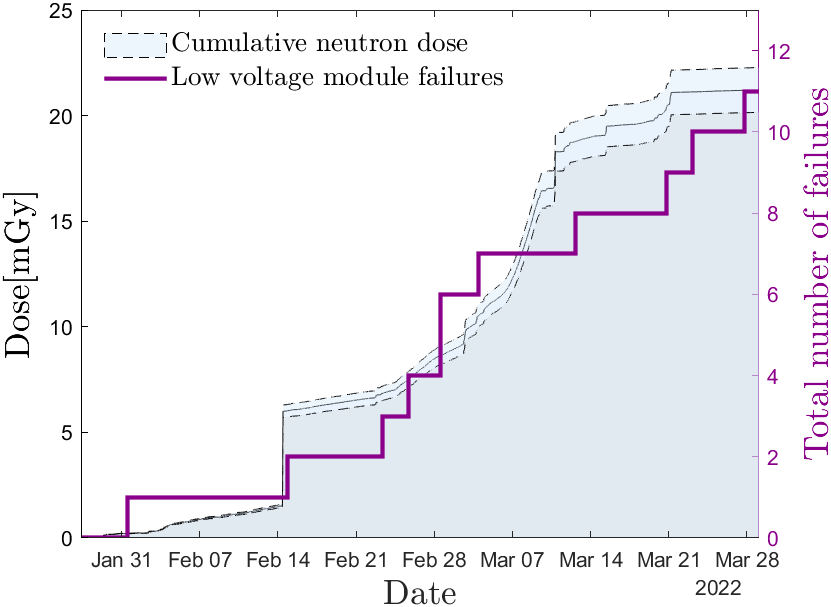
\includegraphics[width=0.6\columnwidth]{Chapter4/images/LV_failure_and_neutronsrate.png}
    \caption{Cumulative neutron dose and \gls{SEE} in the low voltage module}
    \label{fig:lv_neutrons}
\end{figure}
\begin{figure}[!h]
    \centering
    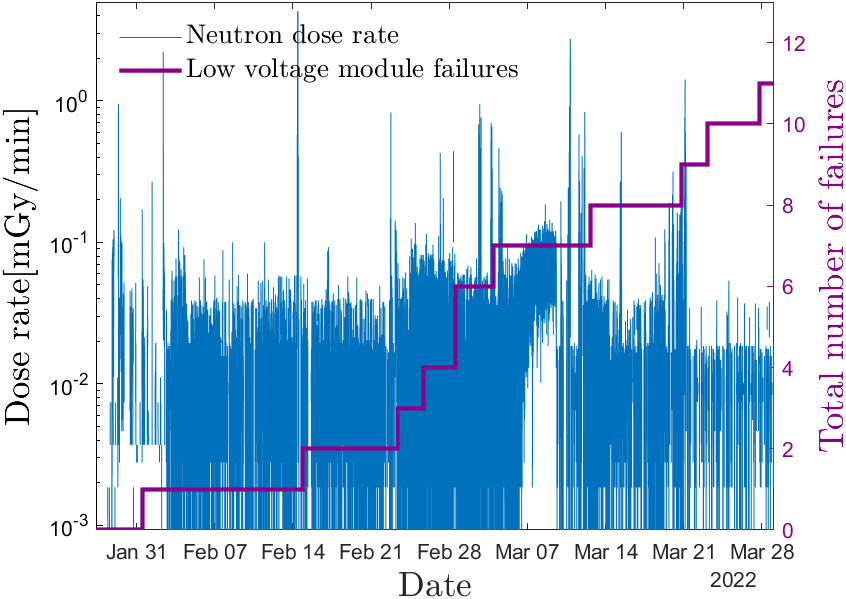
\includegraphics[width=0.6\columnwidth]{Chapter4/images/neutrons_dose_rate.png}
    \caption{Neutron dose rate and failures of the low voltage module}
    \label{fig:lv_neutrons_rate}
\end{figure}
Figure~\ref{fig:lv_neutrons} shows how the number of failures cumulative with the total neutron dose, where the longer periods without failure indicate a break in SIS18 operation. Similarly, Figure~\ref{fig:lv_neutrons_rate} depicts the dose rate and related \gls{SEE}.
For the 11 low voltage module failures, we get the following confidence bands from the Poisson distribution:
   \begin{equation}
  \mathrm{\mu}_{\mathrm{LV}}^{\mathrm{SEE}}=\mathrm{11}_{-3}^{+4}
\end{equation}
Considering the sum of two doses, we get:
\begin{equation}
    \mathrm{D}_{\mathrm{LV}}^{\mathrm{SEE}}=\mathrm{4.45}_{-1.25}^{+1.93}\mathrm{\ mGy}
\end{equation}
Therefore, we can expect a low voltage module failure after $\mathrm{4.45}_{-1.25}^{+1.93}\mathrm{\ mGy}.$ After the occurrence of a soft error in the low voltage module, it was always possible to turn the channels on again.
\newpage
On the other hand, high voltage modules will be placed in an area with lower radiation levels, thus their error sensitivity does not pose a risk to detector operation. In the case of the high voltage module, the \gls{SEE} don't result in a module switch off, but in disabling channels. In two cases all channels were switched off, which is counted as if 15 channels were turned off at the same time. Figure \ref{fig:hv_neutrons} and \ref{fig:hv_neutrons_rate} show the channels' failure rate with the increasing cumulative dose. 
\begin{figure}[!h]
    \centering
    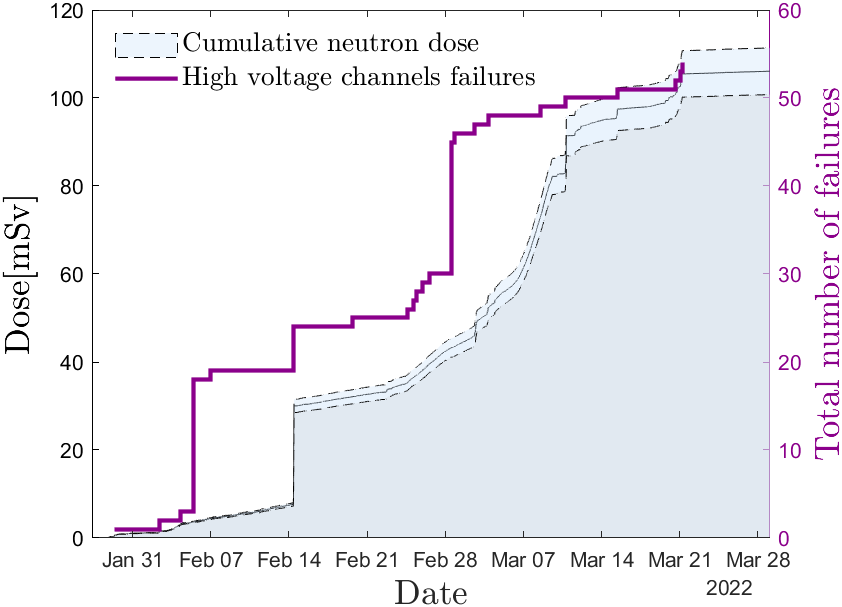
\includegraphics[width=0.6\columnwidth]{Chapter4/images/HV_failure_and_neutronrate.png}
    \caption{Cumulative neutron dose and failures of the high voltage module's channels}
    \label{fig:hv_neutrons}
\end{figure}
\begin{figure}[!h]
    \centering
    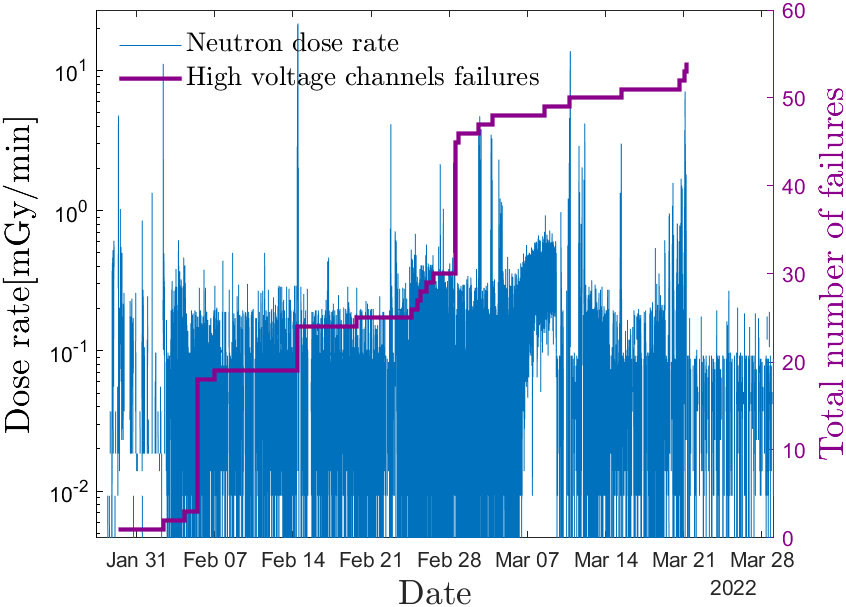
\includegraphics[width=0.6\columnwidth]{Chapter4/images/Hv_neutrons_dose_rate.png}
    \caption{Neutron dose rate and failures of the high voltage module's channels}
    \label{fig:hv_neutrons_rate}
\end{figure}
For the high voltage module, the total number of channels that switched off due to the irradiation is 54. Following a similar procedure as for the previous calculation:
  \begin{equation}
 \mathrm{\mu}_{\mathrm{HV}}^{\mathrm{SEE}}=\mathrm{54}_{-7}^{+8}
\end{equation}
Considering the failure number, it translates to:
\begin{equation}
    \mathrm{D}_{\mathrm{HV}}^{\mathrm{SEE}}=\mathrm{0.91}_{-0.12}^{+0.13}\mathrm{\ mGy}
\end{equation}
If the high voltage module was situated in the same place as the low voltage, we could expect a channel to switch off after $\mathrm{0.91}_{-0.12}^{+0.13}\mathrm{\ mGy}$.
\subsection{Conclusions}
\label{irradiation_results}
The \gls{FEE} of the \gls{STS} will be powered by about 140 low voltage modules. Given that in the worst case some of those modules will be exposed to about 40 mGy/month, the measurement indicates that we can expect about 9 \gls{SEE} per month per module. In practice, it means that every FEB will need to withstand 9 power cycles at low temperatures per month. Assuming operation of 2 months per year and a total projected operating time of 10 years, electronics must withstand at least 180 power cycles. 
\subsection{Potential risk to operation}
If every low voltage module turns off 9 times per month during the operation, the potential consequences need to be carefully assessed. By planning the powering scheme for the \gls{STS}, we can prepare the system for the foreseen power interruptions. In the worst-case scenario, considering that we will use 140 low voltage modules, we can expect about 1260 soft errors a month, which means 1.75 errors per hour.  If there were 16 ROBs connected to one low voltage module, we could experience a temporary shutdown of up to 140 FEBs or 70 modules per hour.  The duration of the shutdown is also critical for the operation. A soft error in the low voltage module can most likely be recovered within seconds, preventing extensive thermal stress in the FEE. On the other hand, for the testing scenarios, we need to consider that the electronics experience full thermal stress, in case fast power recovery is not possible. Additionally, power cycles of the FEE in low temperatures may result in thermally induced mechanical stresses on the components of the PCBs. Hence, the effects of thermal cycling of the FEE should be carefully studied, in order to evaluate the limits in the performance of the electronics  (see section~\ref{thermal_cycling}). Nevertheless, there are also a few methods to decrease the potential risk, both from the radiation-induced damage and potential problems due to thermal shock:
\begin{itemize}
    \item additional radiation shielding material around the power supplies,
    \item powering scheme - for example connecting ROBs and corresponding FEBs to the same low voltage module,
    \item proper software/hardware mechanisms to switch on the channels in a timely manner.
\end{itemize}


\newpage
\section{Thermal cycling of detector electronics}
\label{thermal_cycling}
Operating temperatures inside the \gls{STS} enclosure are dictated by the total non-ionizing dose and noise levels. The temperature conditions in the STS could have repercussions on the functioning of detector electronics. Nevertheless, for the first few years of operation, the ambient temperatures will be higher than \SI{-10}{\celsius}. Operating scenarios of the \gls{STS} together with other constraints related to, for example, the soft errors rate in the low voltage powering of the \gls{FEE}, define the testing procedures for all the electronics which will experience thermally induced mechanical stresses.

One of the elements of the detector module which can experience significant mechanical stresses is the \gls{FEB}.
During the commissioning and operation, the \glspl{FEB} will experience many power cycles. As reported in the~\cite{CBM_PR_2021}, the power cycling of the \glspl{FEB} at room temperature of about \SI{20}{\celsius} run flawlessly, not identifying any issues with the boards. Nevertheless, the testing did not reproduce the STS operational conditions.

To evaluate the behavior of the board in realistic conditions, a thermal cycling setup was envisioned. Thermal cycling testing is usually performed in order to determine the ability of different components and solder interconnects to resist extreme temperature changes. Permanent changes to the electrical or physical features may compromise the detector modules performance.

 For the control and monitoring of devices, as well as for the processing of data the previously developed control framework was introduced. Implementation of the EPICS-based framework played a crucial role, as it enabled live monitoring of many parameters during the tests.

\subsection{Nominal operation scenario of the STS}
\label{nominal}

In the nominal operation scenario at the end of the STS lifetime, the \glspl{FEB} are operated at the nominal power ($\approx8\,W$), and any excess heat is evacuated by cooling liquid (NOVEC 649) is flowing through the \gls{FEB} cooling plate at \SI{-40}{\celsius}. Figure~\ref{fig_coolinkg_block_nominal} and~\ref{fig_nominal_febs}, depict thermal simulations of the cooling plate, \gls{FEB} box, and the \gls{FEB} for the nominal operation scenario.

During periods in which the temperature will change due to transitions between detector states, the electronics will experience thermal stresses, which will partially occur with the electronics switched on. The cases discussed relate to the worst-case scenarios, in which the temperature differences are the highest. 
    
\begin{figure}[!h]
\centering
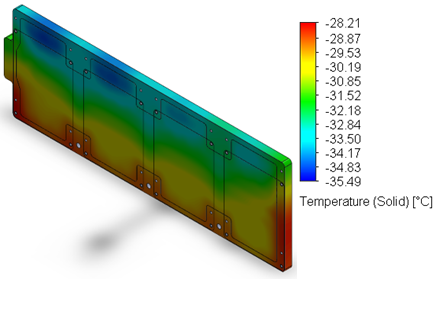
\includegraphics[width=0.6\columnwidth]{Chapter4/images/cooling_block_nominal.png}
\caption{Temperature distribution on the cooling plate for the nominal operation scenario~\cite{Agarwal}.}
\label{fig_coolinkg_block_nominal}
\end{figure}

\newpage

\begin{figure}[!h]
\centering
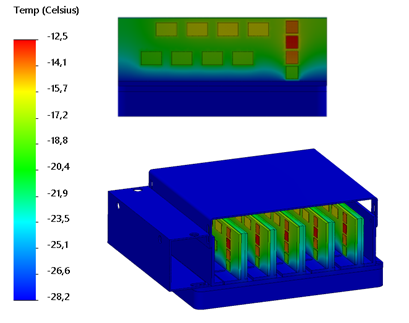
\includegraphics[width=0.62\columnwidth]{Chapter4/images/nominal_febs.png}
\caption{Temperature distribution in the \gls{FEB} box and in the \gls{FEB} for the nominal operation scenario~\cite{Agarwal}.}
\label{fig_nominal_febs}
\end{figure}


During the active, nominal phase of operation, the temperature change of the electronics could be $\Delta T \approx \SI{20}{\celsius}$. This operation mode is summarized in Figure~\ref{fig_nominal_scenario}.  The difference is associated with a slow increase of the coolant temperature from \SI{-40}{\celsius} to \SI{-20}{\celsius}. After switching off the electronics, the temperature reaches the temperature of the cooling plate. The change will be $\Delta T \approx \SI{20}{\celsius}$ (from e.g., \SI{0}{\celsius} to \SI{-20}{\celsius}). These temperatures provide an indication of minimum and maximum thermal cycling set points.  

\begin{figure}[!h]
\centering
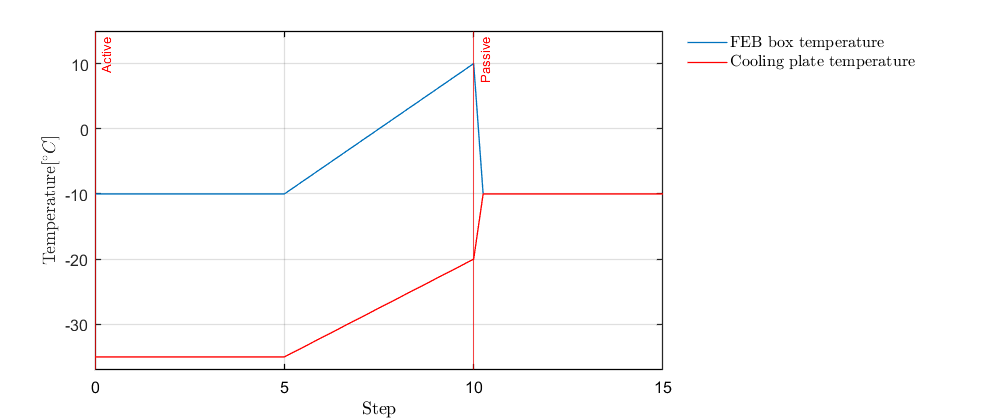
\includegraphics[width=0.85\columnwidth]{Chapter4/images/nominal_all.png}
\caption{An example of \gls{STS} state transition from operation to safe state - comparison of temperatures of a \gls{FEB} box and cooling liquid temperature. A step could be defined as a generic time period.}
\label{fig_nominal_scenario}
\end{figure}


\subsection{Partial shutdown scenario of the STS}
\label{reboot}

At any given point during operation, the operator may need to power cycle a \gls{FEB}(s). In this scenario, the temperature of a given \gls{FEB} may change drastically due to the temporary loss of power. The amount of the thermally induced mechanical stress depends on reboot and configuration time. Besides, in case of a radiation-induced soft error in the power supply, the downtime of a \gls{FEB} may be difficult to predict. If the soft error is instantly recoverable, the FEB will be powered on in seconds after switching off, limiting a deteriorating effect of large temperature changes $\Delta T$.

Figure~\ref{fig_reboot_box} depicts the scenario in which only 5 out of 10 \glspl{FEB} are on, which results in effectively lower temperatures in comparison to the nominal scenario. Nevertheless, the $\Delta T$ remains the same as in the nominal operation scenario. During the operation, this scenario will probably last for a short time (range of seconds), and the temperature of the rebooted \gls{FEB} will not reach as low temperatures as depicted in the previous simulations.


%\begin{figure}[!h]
%\centering
%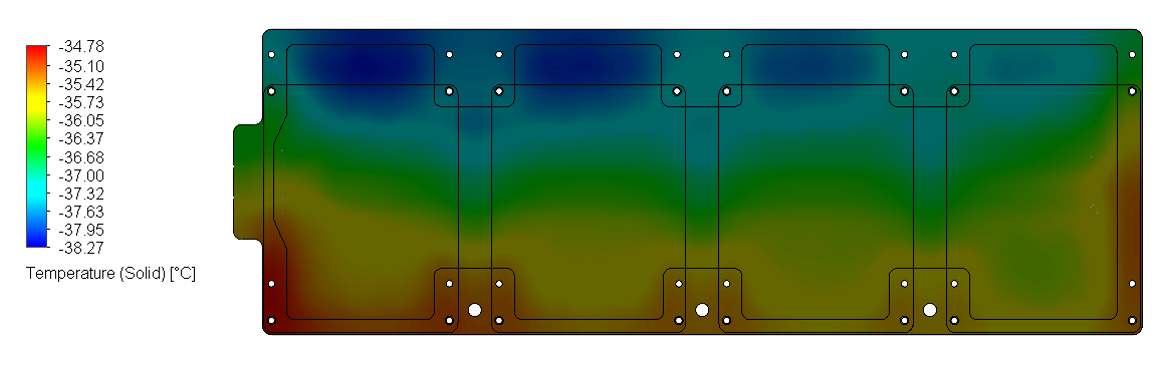
\includegraphics[width=0.85\columnwidth]{Chapter4/images/reboot_cooling_plate.png}
%\caption{Temperature distribution on the cooling plate for the reboot scenario}
%\label{fig_reboot_scenario}
%\end{figure}

\begin{figure}[!h]
\centering
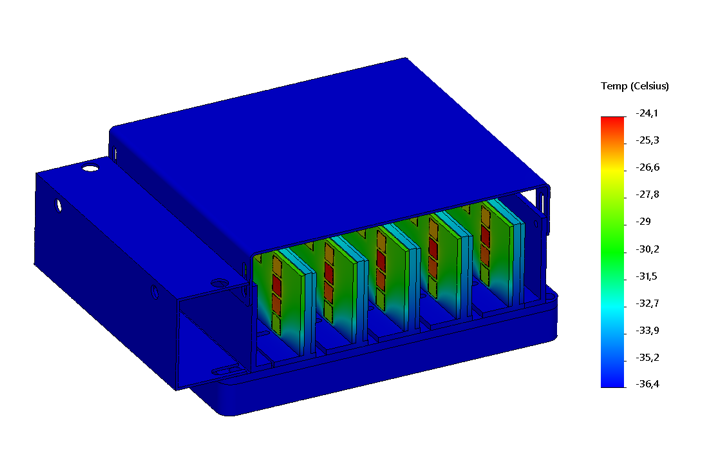
\includegraphics[width=0.57\columnwidth]{Chapter4/images/reboot_box.png}
\caption{Temperature distribution for the partially unpowered \gls{FEB}~\cite{Agarwal}.}
\label{fig_reboot_box}
\end{figure}

\begin{figure}[!h]
\centering
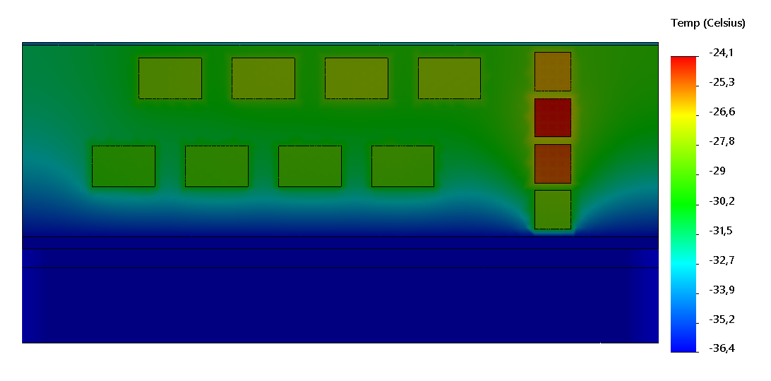
\includegraphics[width=0.6\columnwidth]{Chapter4/images/reboot_FEB.png}
\caption{Temperature distribution of a \gls{FEB} for the partial shutdown scenario~\cite{Agarwal}.}
\label{fig_reboot_FEB}
\end{figure}

\begin{figure}[!h]
\centering
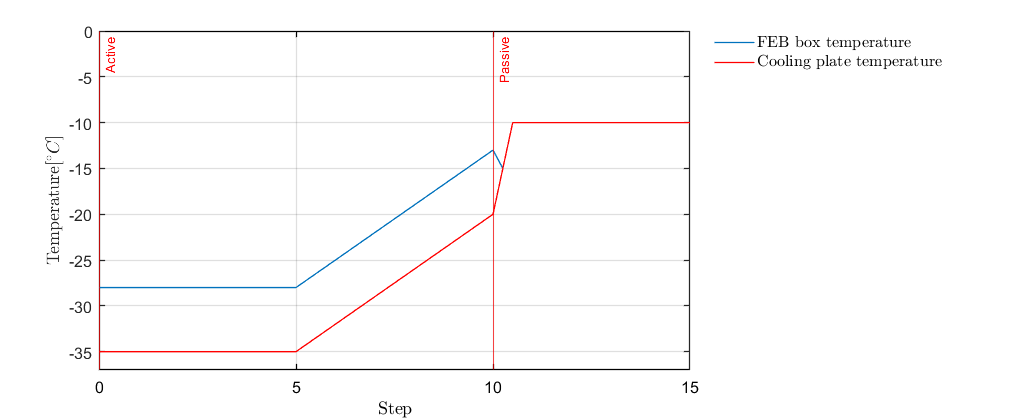
\includegraphics[width=0.85\columnwidth]{Chapter4/images/nominal.png}
\caption{An example of \gls{STS} state transition from operation to safe state - comparison of temperatures of a \gls{FEB} box and cooling liquid temperature.}
\label{fig_reboot_nominal2}
\end{figure}

\subsection{Loss of power scenario of the STS}
\label{power_loss}
The last considered scenario is the so-called loss of power scenario. Out of the three introduced scenarios, it is the least probable one, but it also leads to significant data loss, as 10 \glspl{FEB} would stop sending data. Such a scenario could happen if all the connected low-voltage channels switch off, e.g., due to radiation. In this case, the \glspl{FEB} would reach the temperature of the cooling block ($T \approx \SI{-40}{\celsius}$) if the powering was not turned on within seconds.

\subsection{Influence of the coefficient of thermal expansion on the PCB performance}

The coefficient of thermal expansion (\gls{CTE}) is an important property of materials that affects relative movement between \gls{PCB} components. \gls{CTE} should be a concern when it comes to \glspl{PCB}, as out-of-plane \gls{CTE} could cause cracking and delamination, while in-plane \gls{CTE} may cause for example shear failures in solder joints~\cite{cte_report}. The \gls{STS} \gls{FEB} is equipped with many components which could be the reason for malfunctions at low temperatures, making analysis of potential causes a complex task. 
These components can be seen in Figure~\ref{fig_globtop}.
\begin{figure}[!h]
\centering
\includegraphics[width=0.85\columnwidth]{Chapter4/images/glob_topped_device.png}
\caption{Schematics of the glob-topped device with the materials used for the thermal cycling of different FEB flavors.}
\label{fig_globtop}
\end{figure}

Both the \gls{LDO} regulators and STS-XYTERs are covered with high viscosity glues which are known as glob top\footnote{protective epoxy-based material for microelectronics}. Apart from \gls{CTE}, the performance of the glob top material depends on many other factors:
\begin{itemize}
    \item adhesion to the substrates,
    \item part geometry (including the mass of the components in contact),
    \item temperature extremes,
    \item number of cycles, and transition times.
\end{itemize}


The most common phenomena which cause damage to the glob-topped device are:
\begin{itemize}
    \item wire-bond failure,
    \item failure of the chip to board or substrate joint,
    \item damage to protective chip passivization layer,
    \item chip cracking,
    \item metallization pattern shift,
    \item development of voids or notches in metallization tracks. 
\end{itemize}


According to the data on electronics failures analyzed by the U.S. Air Force over about 20 years, it was shown that 50\% of these failures are related to connectors, 30\% to interconnects, and 20\% to component
parts. Hardware failures may occur due to handling, vibrations, or stress of different origins (including thermal stress). About 55\% of the electronics failures are due to high temperatures and temperature cycling, 20\% of the failures are related to vibration and shock, and 20\% are due to humidity~\cite{thermal_electronics}. 

To protect the STS microelectronics, DYMAX 9001 was the glob top choice for the \glspl{FEB}, and it was then replaced by its successor DYMAX 9014. The \gls{LDO} regulators and \glspl{ASIC} are made of silicon. The linear CTE of glob top materials (DYMAX 9001, DYMAX 9014, DYMAX 9008) and conductive glue (EPO-TEK E4110) is by an order of magnitude higher than the coefficient for the \glspl{PCB} and silicon. Additionally, a volume expansion influences the relative position of different components during thermal cycling.

\begin{table}[!h]
\begin{center}
\caption{Coefficient of thermal expansion of different materials below the glass transition temperature.}
\begin{tabular}{ll}
\hline
\multicolumn{1}{c}{Material} & \multicolumn{1}{c}{CTE $\alpha_{2}$} [\si{\micro\metre\per\metre\per\celsius]}] \\ \hline
DYMAX 9001-E-V3.5~\cite{9001}            & 180                                  \\
DYMAX 9014~\cite{9014}                   & 192                                  \\
DYMAX 9008~\cite{9008}                   & 230                                  \\
EPO-TEK E4110~\cite{4110}                & 150                                  \\ \hline
FR4 (\gls{PCB} material)~\cite{FR4}                          & 15                                   \\
Silicon~\cite{Si}                           & 2.6                                 
\end{tabular}
\label{TCE}
\end{center}
\end{table}

Three main components which need to be analyzed during the testing are the glues (glob top and conductive glue), bonds, and microelectronics (\gls{LDO} regulator and STS-XYTER). From the thermal cycling point of view, power dissipation is one of the key differences between the DC linear voltage regulator and the front-end chip. Figure~\ref{fig_temperatures_camera} depicts the temperature distribution of a powered board. The board was screwed to the cooling plate, which was at \SI{20}{\celsius}.

\begin{figure}[!h]
\centering
\includegraphics[width=0.6\columnwidth]{Chapter4/images/feb_thermal.jpg}
\caption{Temperature of the \gls{FEB} components measured with a thermal camera for the low power consumption scenario, \cite{leo_electronics}. The \gls{LDO} (on the right side of the picture) appear to be hotter than STS-XYTER chips.}
\label{fig_temperatures_camera}
\end{figure}



%\begin{figure}[!h]
%\centering
%\includegraphics[width=0.55\columnwidth]{Chapter4/images/switchoff.png}
%\caption{Sudden loss of power and bringing the \glspl{FEB} back to operation}
%\label{fig_loss}
%\end{figure}

%\newpage
\subsection{Experimental setup for thermal cycling of STS electronics}
\label{cycling_setup}
In order to investigate the effect of thermal cycles of the FEBs, a setup consisting of FEBs, readout board, Lauda chiller, climatic chamber, temperature sensors and humidity sensors was introduced.
A detailed overview of the setup is depicted in Figure~\ref{fig_setup}. The software part features the Control System Studio (Phoebus) for monitoring, accessing the database (Redis DB), and monitoring the \gls{PV}s. Moreover, all values are saved with archiver appliance. The second node features a LabView-based interface for reading out additional humidity sensors. This node was later on depreciated and relative humidity readouts were taken from the built-in Relative Humidity (\gls{RH}) sensor inside the climatic chamber.

The main objective was thermal cycling of the \glspl{FEB}, which consists of 4 LDO regulators (two 1.2\,V LDO and two 1.8\,V LDO regulators) and 8 \glspl{ASIC}. The diagnostic circuit of the STS-XYTER helped to identify \gls{PCB} related malfunctions. In order to read the temperatures, VDDM, and  \gls{CSA} bias values from the chip, a dedicated soft IOC\footnote{purely software-based \gls{IOC}, not connected to any hardware} was deployed. To acquire the previously mentioned values, the pyEPICS library~\cite{pyEPICS} was used, and the GBTxEMU-based readout chain (see \autoref{tester}) was adjusted to publish the values via channel access protocol. 
\begin{figure}[!h]
\centering
\includegraphics[width=0.85\columnwidth]{Chapter4/images/cycling_scheme.png}
\caption{Schematics of the thermal cycling setup. The readout of relative humidity and temperature sensor is realized through Single Board Microcontrollers~(\gls{SBM}) and Raspberry PI. The python interface was developed for both readout chains (ROB and GBTxEMU based). }
\label{fig_setup}
\end{figure}

\newpage
Apart from the \gls{ASIC}-specific values, are other parameters taken into consideration which are as
follows:
\begin{itemize}
    \item currents and voltages supplied to the 1.2\,V and 1.8\,V \gls{LDO} regulators on the \gls{FEB}, 
    \item temperature changes on the T-shelf (as seen in Figure~\ref{fig_cycling_temps}), which are read-out by a Single Board Microcontroller (\gls{SBM}),
    \item humidity and temperature in the climatic chamber (Sensiron SHT85 sensors plus built-in sensors),
    \item set point temperature of the Kryo 51 coolant (used as an alternative for NOVEC)~\cite{KRYO}.
\end{itemize}

There are different glob-top materials that match the \gls{STS} requirements. To get a better understanding of
their performance, \glspl{FEB} with different glob tops were assembled as shown in Figures 7 and 8. Moreover,
to understand the impact of the glob top material, a board without glob top on \glspl{LDO} regulators was
assembled. In total, four different FEB flavors can be distinguished:
\begin{itemize}
    \item with DYMAX 9001 as the glob top (see Figure~\ref{fig_noglobtop}),
    \item with DYMAX 9014 as the glob top,
    \item with DYMAX 9001 as the fill and DYMAX 9008 as the dam \footnote{Dam and fill is a technique for properly covering wire bonded die. It is a two-step method in which a dam is dispensed around the top of the component first, followed by filling the center.} (see Figure~\ref{fig_cycling_temps}), 
    \item without glob top and \glspl{ASIC} (see Figure~\ref{fig_noglobtop}).
    \end{itemize}
%\newpage
\begin{figure}[!h]
\centering
\includegraphics[width=0.45\columnwidth]{Chapter4/images/noglobtop.jpg}
\includegraphics[width=0.45\columnwidth]{Chapter4/images/globtop.jpg}
\caption{The left picture depicts two \glspl{FEB} (version A and B) with the \gls{LDO} regulators covered with 3D-printed protection cap and without glob top. These two boards feature resistors simulating the power consumption of the STS-XYTERs.
The right picture depicts two fully assembled \gls{FEB}s with STS-XYTERS version 2.1 and DYMAX 9001 as the glob top.}
\label{fig_noglobtop}
\end{figure}
\newpage
To prepare for the thermal cycling, the assembled boards (type A and B) were mounted on a cooling shelf (initially with thermal pads, later by gluing it to the T-shelf’s surface) and then eventually placed on a cooling plate in the climatic chamber (see Figure~\ref{fig_cycling_temps}). In order to reproduce similar conditions as in the \gls{STS} (coolant temperature at \SI{-40}{\celsius}) KRYO 51 coolant was used instead of the NOVEC 649 liquid. Additionally, the chamber temperature was always kept below the temperature of the cooling plate to avoid icing. During the cycling, the voltage drop at the \gls{LDO} regulators was the same \SI{0.6}{\volt} for all the boards.

\begin{figure}[!h]
\centering
\includegraphics[width=0.5\columnwidth]{Chapter4/images/FEBB_T_sensors.jpeg}
\includegraphics[width=0.4\columnwidth]{Chapter4/images/thermal_setup.jpeg}
\caption{A \gls{FEB} glued to the T-shelf, with 3 DS18B20 temperature sensors installed on the T-shelf (left) and two \gls{FEB}s mounted on a T-shelf with thermal pads inside a climatic chamber (right).}
\label{fig_cycling_temps}
\end{figure}


\subsection{Testing procedure}
The \glspl{FEB}, Readout Boards (\glspl{ROB}), and  Power Boards (\glspl{POB}) are going to be cooled, and they will experience thermal stress on the components. According to the previously introduced operation scenarios, these boards need to withstand:
\begin{itemize}
    \item without the powering $\Delta T\approx\SI{20}{\celsius} $
    \item with powering $\Delta T\approx\SI{20}{\celsius} $
    \item more than 180 cold startups, as indicated in section~\ref{irradiation_results}
\end{itemize}
To find the operational limits of the boards and reproduce the operation scenarios the testing was divided into three stages: passive cycling, active cycling, and power cycles down to \SI{-40}{\celsius} (so-called cold startup). The transition time between the extreme temperatures (for passive and active cycling) is not manually regulated and is solely determined by the power of the Lauda chiller and the climatic chamber.

The main object of the tests was the \gls{FEB}s and its sensitivity to the thermally induced mechanical stresses. In the two main sets of measurements so far, in total 12 \gls{FEB}s in different configurations were tested.  After each round of thermal cycling (usually 50 cycles), the boards were inspected optically under the microscope for any signs of deterioration or visible changes. On the other hand, during the cycling with powering and low-temperature power cycling, the STS-XYTERs were extensively tested. The \glspl{ASIC} test included configuration of the chip, changing \gls{CSA} values to trigger different current consumption, but also ID consistency check, write/read registers test, and internal pulses. By performing the tests, it is possible to evaluate the performance of the board and estimate the influence of the thermal cycling.

\subsubsection{Passive cycling}
Passive cycling refers to a process of changing the temperature of a tested object in a defined range (e.g., from \SI{-20}{\celsius} to \SI{-10}{\celsius}) without powering. This way the stress on the board and its components is lower. Passive cycling was performed in a series of 50 repetitions between optical and electrical inspection. During this part the following temperature differences were tested:
\begin{itemize}
    \item Set A - 8 \glspl{FEB} (3 \glspl{FEB} type A, 3 \glspl{FEB} type B and 2 \glspl{FEB} without glob top and \glspl{ASIC}) were tested in the realistic operating scenarios of the \gls{STS} [\SI{-20}{\celsius}, \SI{-10}{\celsius}], [\SI{-30}{\celsius}, \SI{-10}{\celsius}], [\SI{-40}{\celsius}, \SI{-10}{\celsius}],
    \item Set B 2 out of 4 \glspl{FEB} (1 out of 2 \glspl{FEB} A and 1 out of 2 \glspl{FEB} B) were tested more extensively by increasing $\Delta T$ - [\SI{-20}{\celsius}, \SI{20}{\celsius}].
\end{itemize}
The \glspl{FEB}, regardless of the type (A or B), are treated equally from the mechanical point of view. The components and the way the boards are assembled are the same.


The characteristic of passive cycling was as follows:
\begin{itemize}
    \item  set B was tested without current trip conditions  and for set A the trip current was set to 3.1 A,
    \item the temperature provided by the Lauda chiller was a few degrees higher than the ambient chamber
    temperature, in order to prevent condensation or icing on the electronics,
    \item the periods at the maximum and minimum temperature were always the same and equaled 20 minutes,
\end{itemize}
No performance deterioration was observed during the passive cycling, which is most likely related to the fact that the boards were previously unused. 
%\begin{figure}[!h]
%\centering
%\includegraphics[width=0.55\columnwidth]{Chapter4/images/active_cycling.png}
%\caption{Example of the thermal cycling (passive) of the FEE}
%\label{fig_passive_cycling}
%\end{figure}

\subsubsection{Active cycling}
Active cycling refers to cycling with the electronics switched on at all times. It was performed in a series of 50 repetitions, but due to the fact that the \glspl{FEB} were powered, all the boards and STS-XYTERs were continuously tested, and the current consumed varied by around 1 A at most. The boards underwent the followings cycles:
\begin{itemize}
    \item set A - 8 \glspl{FEB} - [\SI{-10}{\celsius}, \SI{20}{\celsius}] and [\SI{-40}{\celsius}, \SI{-10}{\celsius}],
    \item Set B - 4 \glspl{FEB} (2 \glspl{FEB} A and 2 \glspl{FEB} B)  $\Delta T$ - [\SI{-20}{\celsius}, \SI{20}{\celsius}], [\SI{-30}{\celsius}, \SI{20}{\celsius}], [\SI{-40}{\celsius}, \SI{20}{\celsius}].
\end{itemize}

\begin{figure}[!h]
\centering
\includegraphics[width=0.65\columnwidth]{Chapter4/images/FEB0ASIC5COMP.png}
\caption{A detailed view on the performed active cycling. The top figure depicts the temperature of the chamber temperature and the set point of the Lauda chiller. Two lower figures show how the readout of temperature and VDDM from a chosen STS-XYTER depends on the cycling temperature. }
\label{fig_active_detailed}
\end{figure}
A detailed view of a few cycles is presented in Figure~\ref{fig_active_detailed}. Figure depicts active cycling from \SI{-30}{\celsius} to \SI{20}{\celsius}. Similarly to passive cycling, the temperature of the cooling block is kept a few degrees (2 -- \SI{3}{\celsius}) above the ambient temperature, although the effective temperature of the active components (STS-XYTERs and \gls{LDO} regulators) is much higher. The two bottom graphs show how the cycling affects the STS-XYTERs diagnostic circuit. The VDDM value varies from about 1200\,mV up to 1240\,mV, but it does not have any effect on the performance of the chip, as the operating range could vary as much as 100\,mV. The measured values of the VDDM may also vary across the \gls{FEB}, which can be seen in Figure~\ref{feb_vary}. These differences emphasize the need to properly calibrate the ADC of the diagnostic circuit, as the measured values should not be too far from the nominal 1.2\,V\footnote{Considering that the voltage drop across the 1.2\,V line connecting the subsequent chips is negligible} supplied by the 1.2\,V \gls{LDO} regulator. 
\begin{figure}[!h]
\centering
\includegraphics[width=0.75\columnwidth]{Chapter4/images/vddm_comp.png}
\caption{VDDM values comparison for different chips in the board. The tests in the chips were performed sequentially, therefore time shift between maxima of  can be seen.}
\label{feb_vary}
\end{figure}

%\newpage
Moreover, during the active cycling, 3 DS18B20 sensors were glued on the T-shelf (see section~\ref{cycling_setup}. The sensors were glued to the T-shelf, in order to determine how the temperature changes when the final thermal interfaces are used (glue between the FEB and T-shelf and carbon composite between the T-shelf and cooling block). Figure~\ref{fig_active_sensors} depicts the difference between the temperatures measured by different sensors during cycling. 

\begin{figure}[!h]
\centering
\includegraphics[width=0.75\columnwidth]{Chapter4/images/active.png}
\caption{Temperature evolution of the T-shelf during the active cycling. The DS18B20 \cite{DS18B20} sensor has an uncertainty of $\SI{0.5}{\celsius}$.}
\label{fig_active_sensors}
\end{figure}

\newpage
Temperature sensor 1 was placed above the \gls{LDO} regulators, therefore the measured values are always higher than for the two other sensors. Temperature sensor 2 was placed on top of the T-shelf but on the other side of the board. Sensor 3 was placed on the side of the T-shelf next to the powering services, its temperature is significantly lower, what is clearly visible at \SI{-38}{\celsius}, as it is placed closer to the heat exchanger (the cooling plate). This behavior was also confirmed by the simulations - see Figure~\ref{fig_nominal_febs} and Figure~\ref{fig_reboot_FEB}. 


%\newpage

\subsubsection{Low-temperature power cycling}
On contrary to the two introduced thermal cycling methods, power cycling is performed at a stable temperature. After switching the power on at low temperature, the \glspl{FEB} functionalities are tested and the power supply output is switched off. This process is then repeated a few hundred times. 

Power cycling at low temperatures is considered as one of the riskiest events that may cause a board to fail.  As identified during the irradiation of the power supplies, we should expect at least 180 radiation-induced soft errors in the low-voltage modules. Radiation-induced phenomena (latchup in the chips, and soft errors in the powering units) limit the lifetime of the electronics and could cause the boards to fail over time. \glspl{FEB} will also be power cycled during testing, commissioning, and operation of the detector, increasing the total number of power cycles up to two/three times. The previously introduced \glspl{FEB} underwent the following power cycling in low temperatures:
\begin{itemize}
    \item set A - 4 \glspl{FEB} - 200 cycles at $T = \SI{-30}{\celsius}$, 4 other \glspl{FEB} (including the one without chips) 300 cycles at $T = \SI{-30}{\celsius}$,
    \item Set B - 2 \glspl{FEB} - 50 cycles at $T = \SI{-20}{\celsius}$, 2 other \glspl{FEB} 50 cycles at $T = \SI{-30}{\celsius}$.
\end{itemize}
Figure~\ref{fig_power_cycle} shows how the current drawn by the 1.2~V \gls{LDO} regulators and 1.8~V \gls{LDO} regulators changes in the course of different tests performed in the STS-XYTERs. The highest current values (for the 1.2\,V LDO regulator) are reached during write/read tests of the registers. The changes of the 1.2\,V LDO regulator current are related to the changes of the \gls{CSA} values during testing. During one run of the testing script, the \gls{CSA} changes from 5 to 31 (the most probable range for the chip during STS operation). 
\begin{figure}[!h]
\centering
\includegraphics[width=0.6\columnwidth]{Chapter4/images/currents.png}
\caption{Cold startup of one of the \gls{FEB}: current consumed by the 1.8~V and 1.2~V \gls{LDO} regulators during the test procedure. During the period, in which the power is on, each chip undergoes 3 testing cycles.}
\label{fig_power_cycle}
\end{figure}
\subsection{Results and onset of failure analysis}
Already during preliminary thermal cycling activities (not discussed in this thesis), it was determined that the \glspl{LDO} are more prone to fail than the STS-XYTERs. Therefore, the main effort was put to gain statistics by testing multiple boards and to identify the onset of a potential \gls{LDO} regulator-related failure. To get a better understanding of the conditions leading to failures, the two sets (A and B) of measurements were compared. 


In the case of set A, which featured 8 \glspl{FEB}: 4 \glspl{FEB} with DYMAX 9001, 2 \glspl{FEB} with DYMAX 9008 as the DAM and 9001 as the fill, and 2 \glspl{FEB} without STS-XYTERs and globtop over the \gls{LDO} regulators, during the passive cycling and active cycling no failure was observed. No deterioration was observed under the microscope. First failures were detected during the power cycling at $T=\SI{-30}{\celsius}$, as summarized in Table~\ref{tab:SetA}. 

\begin{table}[!h]
\centering
\caption{Detailed description of the \gls{LDO} failure with regard to the type and number of cycles.}
\resizebox{\textwidth}{!}{%
\begin{tabular}{lll}
Globtop                   & Failure Appearence             & Remarks                       \\ \hline
DYMAX Dam 9008, fill 9001 & $\approx$ 100 power cycles     & 1.8\,V \gls{LDO} failure (AVVD18)      \\ \hline
DYMAX 9001                & $\approx$ 200 power cycles     & 1.2\,V \gls{LDO} failure after cycling  \\ \hline
DYMAX 9001                & $\approx$ 200/300 power cycles & 1.2\,V \gls{LDO} failure during cycling \\ \hline
\end{tabular}%
}
\label{tab:SetA}
\end{table}
The onset of the \gls{LDO} failure can be seen in Figure \ref{fig_cold_startup}. At about \SI{500}{\minute} the 1.2\,V LDO regulator input current started dropping, indicating increasing resistance in the circuit. As depicted in Figure \ref{fig_cold_startup} once the temperature reached $\SI{20}{\celsius}$ the current consumption was again nominal. After about  3000\,min, this effect turned out to be irreversible, and we observed the complete failure of the 1.2\,V \gls{LDO} regulator. After about 100 cycles, the current consumption measured at the level of the power supply dropped to almost 0\,A. 
%\newpage
\begin{figure}[!h]
\centering
\includegraphics[width=0.46\columnwidth]{Chapter4/images/currents_long.png}
\includegraphics[width=0.48\columnwidth]{Chapter4/images/cycling.png}
\caption{Current consumed by the 1.8\,V and 1.2\,V \gls{LDO} regulators during the cold startup testing at $T = \SI{-30}{\celsius}$ (left)
Comparison of the lauda chiller setpoint, readouts from the internal temperature and relative humidity sensors of the climatic chamber (right).}
\label{fig_cold_startup}
\end{figure}

Similarly, the onset of the \gls{FEB} malfunction can be seen in the diagnostic circuit of the STS-XYTER (see figure \ref{fig_active_failure}). VDDM drops significantly, at the point at which the \gls{LDO} stops providing the nominal current. The temperature measured by the chip drops by $\SI{15}{\celsius}$, and the VDDM reaches 0\,mV, indicating a problem with 1.2\,V \gls{LDO} regulator It was later identified that one of the bond connections of the \glspl{LDO} pad got detached from the board due
to thermal stress. Therefore, the output current of the \gls{LDO} was reduced to a few mA and the voltage was not delivered to the Analog Frond End of the \glspl{ASIC}. 

% Please add the following required packages to your document preamble:
% \usepackage{graphicx}
\begin{table}[!h]
\centering
\caption{Detailed description of the \gls{LDO} failure with regard to the type and number of cycles}
\label{tab:setB}
\resizebox{\textwidth}{!}{%
\begin{tabular}{llll}
\textbf{Globtop} & Cycles                                                                                                                                                                                                                                                                                  & Failure                                                                                                     & Remarks                                                                                              \\ \hline
DYMAX 9001       & \begin{tabular}[c]{@{}l@{}}50 passive cycles {[}$\SI{-20}{\celsius}, \SI{20}{\celsius}${]}\\ 50 active cycles {[}$\SI{-20}{\celsius}, \SI{20}{\celsius}${]}\\ 50 cold startups at $T=\SI{-20}{\celsius}$\end{tabular}                                                                   & \begin{tabular}[c]{@{}l@{}}43th active cycle \\ {[}$\SI{-30}{\celsius}, \SI{-20}{\celsius}${]}\end{tabular} & 1.2\,V \gls{LDO} failure                                                                             \\ \hline
DYMAX 9001       & \begin{tabular}[c]{@{}l@{}}50 passive cycles {[}$\SI{-20}{\celsius},\SI{20}{\celsius}${]}\\ 50 active cycles {[}$\SI{-20}{\celsius}, \SI{20}{\celsius}${]}\\ 50 cold startups at $T=\SI{-20}{\celsius}$, \\ 50 active cycles {[}$\SI{-30}{\celsius}, \SI{20}{\celsius}${]}\end{tabular} & \begin{tabular}[c]{@{}l@{}}40th cold startup at \\ $T=\SI{-30}{\celsius}$\end{tabular}                      & \begin{tabular}[c]{@{}l@{}}failure of both 1.2\,V \gls{LDO}s\\ 1.8\,V \gls{LDO} failure\end{tabular} \\ \hline
DYMAX 9001       & \begin{tabular}[c]{@{}l@{}}50 passive cycles {[}$\SI{-30}{\celsius}, \SI{20}{\celsius}${]}\\ 50 active cycles {[}$\SI{-30}{\celsius}, \SI{20}{\celsius}${]}\end{tabular}                                                                                                                & \begin{tabular}[c]{@{}l@{}}29th cold startup \\ {$\SI{-40}{\celsius}$}\end{tabular}                         & 1.2\,V \gls{LDO} failure                                                                             \\ \hline
\end{tabular}%
}
\end{table}
%\newpage


\begin{figure}[!h]
\centering
\includegraphics[width=0.6\columnwidth]{Chapter4/images/FEB2ASIC2COMP1.png}
\caption{Temperature and VDDM of a chosen STS-XYTER, and the onset of \gls{LDO} regulator failure.}
\label{fig_active_failure}
\end{figure}

One of the potential failure mechanisms can be seen in Figure~\ref{fig_ldo_lift}. An air bubble seen on the right photo caused the regulator to lift from the \glspl{PCB} surface, resulting in bond breaks. Hence, the \gls{LDO} was not providing the nominal voltage and current to the chips. 

\begin{figure}[!h]
\centering
\includegraphics[width=0.8\columnwidth]{Chapter4/images/FEB_81_LDO_lift.png}
\caption{Microscopic view of the air bubble between glob top and bonds of the \gls{LDO}.}
\label{fig_ldo_lift}
\end{figure}
%\newpage
\subsection{Conclusions}
The deployed part of the developed EPICS-based framework for the thermal cycling of the \gls{STS} electronics enabled automation of the cycling process, storing the necessary data and analyzing it in order to evaluate the capabilities of the \glspl{FEB}. 

In total 12 \glspl{FEB} were investigated in order to find the boundary conditions for the temperature operation range. Performed thermal investigations led to discovering the limits of the \glspl{FEB}, namely failures related to the \gls{LDO} regulators. The realized measurements led to 6/24 1.2\,V \gls{LDO} failures and 2/20 1.8\,V \gls{LDO} regulator-related failures. The more frequent 1.2\,V \gls{LDO} regulator failure can be associated with larger current changes, leading to larger temperature differences. Furthermore, the boards initially tested in harsher conditions (bigger difference between the extreme temperatures) tend to fail sooner. Moreover, the \glspl{FEB} without \glspl{ASIC} and globtop on the LDO regulator didn’t show any sign of malfunction. Nevertheless, due to the lack of \glspl{ASIC}, it was impossible to change the analog line current.

As described in the introduction to thermal cycling, one of the most probable mechanisms leading to the \gls{LDO} regulator-related failure is the mismatch of the \gls{CTE}. It may potentially result in failure of the \gls{LDO} regulator due to e.g., the lift of bonds.

Findings in this section obtained through the deployed control system architecture provide crucial information on how to improve the module and their performance before the mass production of the modules for the final \gls{STS}. 

%\begin{figure}[!h]
%\centering
%\includegraphics[width=0.6\columnwidth]{Chapter4/images/temps.png}
%\caption{A power cycle}
%\label{fig_cold_startup}
%\end{figure}

%\begin{figure}[!h]
%\centering
%\includegraphics[width=0.6\columnwidth]%{Chapter4/images/csa.png}
%\caption{A power cycle}
%\label{fig_cold_startup}
%\end{figure}

\newpage
\chapter{Solutions for the humidity monitoring in STS}
\label{chap:fos}
The third test activity, which involved important research for the \gls{STS} is related to the testing of different relative humidity and temperature sensors. Due to the harsh conditions in the detector, the sensor's choice is an important task that will ensure the proper safety and operation of the system. This chapter presents the overview of different solutions for ambient sensing, together with answers to whether the tested technology meets all the requirements. Most efforts were made to characterize fiber optic sensors, and subsequently come up with safety requirements and systems that would address potential risks posed by e.g. too humid environment. 

\section{Sensors requirements}

The design of the \gls{STS} \cite{Heuser:54798} defines the requirements for ambient sensors. As described in the section~\ref{cooling}, the ambient temperature will reach \SI{-10}{\celsius} at the end of the \gls{STS} lifetime. The cooling liquid (3M NOVEC 649) will be circulating at temperatures close to~\SI{-40}{\celsius}. Therefore, the first boundary condition arises - the frost point needs to be below~\SI{-40}{\celsius} to avoid ice formation or condensation on the \gls{FEE}. For the first few years of operation, the temperatures will be higher and therefore RH/frost point can be measured more accurately. One of the most common techniques to achieve the frost points below~\SI{-40}{\celsius} is baking. In the case of the silicon tracker, too high temperatures could destroy the~\gls{FEE}. 
During the detector's lifetime (10 years), there will be limited opportunities to perform any upgrades. Therefore, the sensors have to withstand the radiation accumulated during that period. As some of the sensors can be placed in the vicinity of the beam pipe, the total dose could reach more than 10~kGy. The humidity measurements will be distributed, implying that different sensors may face different doses. As the detector will be placed in a dipole magnet providing a magnetic field of \SI{1}{\tesla\metre}, the sensors need to be insensitive to it. An ideal humidity sensor should meet the following requirements:
\begin{itemize}
    \item small dimensions and mass (especially when placed close to the active area of the system),
    \item accurate relative humidity readouts at temperatures down to~\SI{-20}{\celsius}, 
    \item ideally respond to a wide range of \gls{RH} values from 0~\% to 80~\%,
    \item high repeatability and low hysteresis,
    \item reliable operation across long distances (the readout device needs to reside at least~\SI{20}{\metre} away from the detector).
\end{itemize}

On the other hand, due to overpressure conditions inside the \gls{STS} enclosure, a low response time (seconds) is not necessarily needed. For the hardware and software interlocking, a delay of up to minutes is considered to be acceptable. The purpose of this chapter is to discuss the considerations for a distributed sensing system, as well as the extensive testing and design of fiber optic sensors. 
\section{Vapor pressure and its significance}

The relative humidity or the dew/frost point, are commonly used indicators to describe the number of water molecules in the air. Nevertheless, the dew/frost point is a much more useful value, as it provides an absolute value. The temperature at which water vapor in any gas medium (at constant pressure) begins to condense into liquid water or solid ice at the same rate at which it evaporates, which is a measure of how much water vapor is in a gas medium, is known as the dew/frost point. Water vapor condenses as liquid water at gas temperatures above \SI{0}{\celsius} (dew). A dew point is defined as a liquid condensation layer. Water vapor condenses as solid ice at gas temperatures far below \SI{0}{\celsius} (frost). A frost point is defined as a solid condensation layer. However, for gas temperatures ranging from \SI{0}{\celsius} to approximately \SI{-20}{\celsius}, the state of the condensed layer is unknown; it could be either water, ice, or a combination of both \cite{nie_dewpoint}. 


The first documented formula for vapor pressure (over water and over ice) was introduced by Goff and Gratch in 1945 \cite{goff_gratch}. The original correlation (over water) is as follows:

\begin{equation}
\begin{split}
    &log({e}^{*}_{s}) = a(T_{st}/T - 1) + b(log(T_{st}/T) - c(10^{11.344(1-T/T_{st})} - 1) \\
    &+ d(10^{-3.49149(T_{st}/T - 1} -1) + log(e^{*}_{st})
\end{split}
\end{equation}
where: log refers to the logarithm in base 10, $e_{s}$ is the saturation water vapor pressure~(hPa), a to d are constants; $a = - 7.90298$, $b=5.02808$, $c=1.3816*10^{-7}$, $d=1.3816*10^{-7}$, $e^{*}_{s}$ is the stream-point pressure ($1013.246~hPa$), and $T_{st}$ is the boiling point (at 1~atm) temperature (373.15~K). A similar equation can be also formulated for the vapor pressure over ice. These equations marked the beginning of the tries to formulate a highly accurate description of water dynamics. In this chapter, a highly accurate empirical formula was used to estimate the dew point. The Magnus formula is much simpler to use and allows to convert between the saturation vapor pressure and temperature with minimal error~\cite{magnus}: 
\begin{equation}
    e^{*}_{s} = c*e^{(aT/(b+T))}
\end{equation}
where: 
The \gls{RH} is usually defined as the ratio of the water vapor pressure ($p$) to the equilibrium vapor pressure over a plane of water ($p_{s}$):
\begin{equation}
    RH = 100\frac{e}{e^{*}_{s}}
    \label{eq:RH}
\end{equation}
Based of the parameters approximations by Sonntag ($c=6.112$~hPa, $a=17.62$, $b=243.12$~\SI{}{\celsius}) \cite{magnus}, the formula converges to:
\begin{equation}
    e^{*}_{s} = 6.112*e^{(17.62T/(243.12))}
    \label{eq:pressure}
\end{equation}
The dew formation corresponds to the equation:
\begin{equation}
    e^{*}_{s}(T_{d}) = e_{st}(T)
    \label{eq:dew}
\end{equation}
This approximation provides an maximum error of \SI{0.35}{\celsius} between \SI{-45}{\celsius} and \SI{60}{\celsius} in comparison to the more complex formula described in \cite{hardy}. 
Inserting the equation \ref{eq:RH} and \ref{eq:pressure} to the \ref{eq:dew} leads to the formula below, which provides the dew point in \SI{}{\celsius}.
\begin{equation}
    T_{d}(T, RH) = \frac{\lambda(ln(\frac{RH}{100})+\frac{\beta T}{\lambda + T})}{\beta - (ln(\frac{RH}{100})+\frac{\beta T}{\lambda + T}}
    \label{eq:td}
\end{equation}
The dew points based on relative humidity and temperature can be seen in the figure~\ref{fig:dewpointmagnus}.
\begin{figure}[!h]
\centering
\includegraphics[width=0.65\columnwidth]{Chapter5/images/dewpointmagnus.png}
\caption{Dew points calculations based on the empirical formulas}
\label{fig:dewpointmagnus}
\end{figure}
In order to compare the results of different relative humidity sensors and dew points sensors, uncertainties of the \footnote{"Dry Bulb Temperature" refers essentially to the ambient air temperature. It is called "Dry Bulb" because the air temperature is indicated by a thermometer not affected by the moisture of the air.}{dry-bulb} temperature and \gls{RH} are needed. In uncertainty analysis, the individual standard uncertainty $\mu$ is defined as the uncertainty of the result of a measurement expressed as its standard deviation~\cite{NIST_1994}. Hence, assuming the rectangular uncertainty for the sensors that measure the temperature and relative humidity:
\begin{equation}
    \mu(x_{i}) = \frac{a}{\sqrt{3}}
\end{equation}
where a is the uncertainty available in the datasheets, and $u_{i}$ represents the measured value. The combined uncertainty $\mu_{c}$ can be derived from equation \ref{eq:dew} based on the law of propagation of uncertainty~\cite{dp_uncertainty}:
\begin{equation}
    u_{Td} = \left [  \left (\frac{\partial T_{d}}{\partial T_{a}}  \right )^{2} \mu^{2}(T) + \left (\frac{\partial T_{d}}{\partial RH}  \right )^{2} \mu^{2}(RH)\right ]^{1/2}
    \label{dp_error}
\end{equation}
In each system, we assume that measuring dew point temperature or relative humidity is statistically independent of measuring air temperature and the confidence level for the uncertainty interval is 68~\%.  Moreover, below~\SI{0}{\celsius} the frost point starts to play a key role. The moisture in the air will undergo deposition as a layer of frost on exposed surfaces that are also at a temperature below the frost point. 

\section{Overview of different technologies}

Nowadays electronic humidity sensors are commonly used in industry, scientific research facilities, and civil infrastructure. In general, we can divide the sensors based on their operating principle - changes in current, voltage, weight, or conductivity can be subsequently associated with humidity changes if the underlying detection principles relate to interaction with water. Resistive and capacitive sensors represent over 75~\% of all sensors used today. As the names indicate their working principles are based on capacitance and resistance changes respectively. The two most difficult requirements to be met are radiation hardness and insensitivity to the magnetic field. Radiation can affect sensor materials in different ways depending on their type, rate of interaction, and material composition. Sensor structures are affected by radiation due to modifications to their lattice structures. For example, capacitive sensors like HIH3610 and HIH4030 tested in CERN turned out to be critically damaged after irradiation~\cite{Berruti} On the other hand, recently it was also reported that capacitive sensors from IST AG has a linear response to the radiation, what can be easily corrected~\cite{Kapic_sensor}. Employing such sensors in a \gls{HEP} experiment, especially in a tracker which is surrounded with a magnet raises questions about the sensitivity to the magnetic field. One of the possible solutions is using fiber optic-based sensors which are by design not sensitive to the changing magnetic field. Another possibility would be to transfer the air from the detector enclosure to measure it outside of the magnetic field, in an area without elevated dose. 

The efforts to employ miniaturized sensors in the \gls{HEP} experiment have been ongoing for many years \cite{Berruti}. A general review of the dew point and relative humidity sensing techniques was presented in~\cite{RITTERSMA}. On the other hand, a more recent overview with a case-specific study related to \gls{HEP} is summarized in \cite{Kapic}. The \gls{STS} will feature a few different technologies of the \gls{RH} and temperature sensors - capacitive sensors, fiber optic sensors and dew point transmitters. 


\subsection{Industrial capacitive sensors}
The capacitive sensors, in the simplest form, can be made out of two parallel plates, where the capacitance between the two electrodes in given by:
\begin{equation}
C = \epsilon_{r}\epsilon_0\frac{A}{d}
\end{equation}
where the $\epsilon_{r}$ and $\epsilon_{0}$ are the relative and vacuum permittivity constant, A is the plate surface area and d is the plate distance. If the humidity changes can be associated to the changes of one of the parameters a \gls{RH} can be therefore calculated. 
The capacitive \gls{RH} sensors can measure below \SI{0}{\celsius}, they are fairly miniaturized and insensitive to pressure changes. The main drawbacks of these sensors are listed below:
\begin{itemize}
    \item limited long-term stability,
    \item sensitive to water condensation,
    \item limited distance to the readout device,
    \item most of the sensors are not radiation-hard.
\end{itemize}
Two different \gls{RH} capacitive sensors have been tested in low-temperature regimes - IST HYT221 and Sensiron SHT85. Figure \ref{fig:hyt221} shows the \gls{RH} and temperature error respectively. Measuring humidity at low temperatures below \SI{-20}{\celsius} and 5~\% \gls{RH} leads to large dew point errors (\SI{7}{\celsius} and more). The estimated dew point errors are presented in figure \ref{fig:hyt221_dp}.
\begin{figure}[!h]
\centering
\includegraphics[width=0.85\columnwidth]{Chapter5/images/hyt221_rh.png}
\caption{Relative humidity and temperature uncertainties \cite{hyt221}}
\label{fig:hyt221}
\end{figure}
\begin{figure}[!h]
\centering
\includegraphics[width=0.6\columnwidth]{Chapter5/images/HYT221RH7T15.png}
\caption{Dew point error based on values from the figure \ref{fig:hyt221}}
\label{fig:hyt221_dp}
\end{figure}
\newpage
Figure \ref{fig:sht85} shows the uncertainties for the measurements with the SHT85 sensor above \SI{0}{\celsius}. The data below \SI{0}{\celsius} is not provided, therefore an extrapolation was made in order to have a comparison with the HYT221 sensor. The results are presented in the figure~\ref{fig:sht85_dp}. In this case, the errors reach up to \SI{7}{\celsius} in the lowest temperatures and \gls{RH} levels.
\begin{figure}[!h]
\centering
\includegraphics[width=0.65\columnwidth]{Chapter5/images/sht85_rh.png}
\caption{Relative humidity uncertainties, the temperature uncertainty is \SI{0.2}{\celsius} \cite{SHT85}}
\label{fig:sht85}
\end{figure}

\begin{figure}[!h]
\centering
\includegraphics[width=0.6\columnwidth]{Chapter5/images/SHTRH15T02.png}
\caption{Dew point error based on the the figure \ref{fig:sht85}}
\label{fig:sht85_dp}
\end{figure}
\newpage
The results presented above don't take into consideration additional effects that alter the dew point results, like hysteresis or drift, which could together contribute by 1~\% or more to the \gls{RH} measurement. Moreover, the performance of the SHT85 is most likely also worse in the low-temperature regime. The comparison of the industrial capacitive sensors shows a large performance disproportion which is also reflected in the price. In general, the industrial capacitive sensors are much cheaper than the custom trace humidity measurement systems or fiber optic sensors. Nevertheless, the readout of such sensors may be affected by the radiation and magnetic field, so they can't be considered as a reliable solution for a long-term operation in the \gls{STS}. The next type of sensors that yield promising results is fiber optic sensors~\ref{FOS}.

\subsection{Fiber optic sensors}
\label{FOS}
Optical fiber optic sensors-based system usually consists of three main components as optical source, transducer, and detector. In general, the sensing principle relies on modifying one or more properties of light (most commonly a laser, diodes, or LEDs are employed as the optical sources) passing through a transducer which is located inside the fiber. A schematic view of a sensing setup is presented in the figure~\ref{fig:sensing}.  The mentioned figure highlights also another feature of this technology, distributed sensing or even continuous sensing offers the unique opportunity for many sensing points in one fiber~\cite{GRATTAN200040}. 
\newpage
\begin{figure}[!h]
\centering
\includegraphics[width=0.95\columnwidth]{Chapter5/images/sensing.png}
\caption{Comparison of different sensing possibilities with the \gls{FOS}}
\label{fig:sensing}
\end{figure}

In general, humidity sensing can be classified according to the operating principles being used \cite{fos_overview}. Furthermore, we can distinguish intrinsic and extrinsic sensors that indicate whether sensing occurs inside or outside of the fiber. The main effort has focused on in fiber grating sensors, which belong to a class of intrinsic \gls{FOS} that has gained popularity in recent years. As a result, we initially focused on a technology called Fiber Bragg Grating. The driving factor for this decision was the successful implementation of the sensors in the Compact Muon Solenoid (\gls{CMS}), which was extensively reported in a number of papers and summarized in the PhD thesis~\cite{Berruti}.

Fiber optic sensors have notable advantages in comparison to conventional sensors:

\begin{itemize}
    \item fibers can be insensitive to radiation or have a predictable behavior,
    \item magnetic field insensitive,
    \item good signal transmission over long distances,
    \item multiplexing capabilities (see figure~\ref{fig:sensing}),
    \item immunity to electrostatic and electromagnetic interference,
    \item resistant to harsh conditions - the sensors are completely passive elements, hence they offer long durability.
\end{itemize}
On the other hand, \gls{FOS} are difficult to integrate into hardware interlocks, and handling and installation of the sensors might be more challenging due to the risk of damaging the fiber.




\subsubsection{Fibre Bragg Grating based sensors}

Fiber Bragg Grating is a type of selective filter that reflects light signals at a specific wavelength known as the Bragg wavelength. Such a filter is created by inscribing a systematic variation of the refractive index~\cite{fbg_overview}. This characteristic wavelength ($\lambda_{B}$) is dependant on the fiber effective refractive index ($\eta_{eff}$) and the grating pitch ($\Lambda$) of the \gls{FBG}~\cite{Othonos2000FiberBG}:
\begin{equation}
    \lambda_{B} = 2 \eta_{eff} \Lambda
\end{equation}
Both factors can be affected by strain, temperature, magnetic field, and/or pressure changes, which makes them a viable choice for sensing applications~\cite{Yun-Jiang_Rao_1997}. In general wavelength shift $\lambda_{B}$ can be formulated as:
\begin{equation}
    \frac{\Delta\lambda_{B}}{\lambda_{B}}=(1-P_{e}) \epsilon + \left [(1-P_{e}) \alpha + \xi  \right ] \Delta T
\end{equation}
where $P_{e}$ is a photo-elastic constant, $\epsilon$ is a strain induced on the fiber, $\alpha$ is the thermal expansion coefficient of the coated \gls{FBG}, and the $\xi$ is the thermo-optic coefficient of the fiber. Using an \gls{FBG} temperature sensor requires decoupling the strain measurement from the temperature measurement, usually called temperature compensation~\cite{Yun-Jiang_Rao_1997}. The most commonly used solution involves using two sensors next to each other or inscribed in the same fiber. The first sensor is responsible for measuring the strain, and the second one measures the temperature in strain-free conditions. The wavelength shift $\Delta \lambda$ induced by the $\Delta T$ can be described as:
\begin{equation}
    \frac{\Delta\lambda_{B}}{\lambda_{B}}=\left [(1-P_{e}) \alpha + \xi  \right ] \Delta T
\end{equation}


\begin{figure}[!h]
\centering
\includegraphics[width=0.45\columnwidth]{Chapter5/images/Picture1.png}
\caption{FBG-based sensors for relative humidity measurements}
\label{fig:fbg_scheme}
\end{figure}


It's possible to measure RH instead of strain by applying a hygroscopic material (for example, polyimide) to the fiber cladding (see figure~\ref{fig:fbg_scheme}. The  Bragg wavelength shift becomes a superposition of temperature and humidity effects in this case (see equation (see equation~\ref{eqn:FBG})~\cite{Kronenberg:02, YEO2008280}. 
                            %\newpage
                             \begin{equation}\label{eqn:FBG}
                            %\large
                                    \frac{\Delta\lambda_{B}}{\lambda_{B}}=\Delta TS_{T}+\Delta RHS_{RH}
                            \end{equation}
                            where $\lambda_{B}$ is the Bragg wavelength, and $S_{RH/T}$ are the sensitivity coefficients for RH and temperature, respectively. 

Similarly to the strain measurement, it’s crucial to have precise temperature readouts in the vicinity of the coated \gls{FBG}. Otherwise, the actual RH readout may be dominated by uncertainty or just the inaccurate temperature measurement. \gls{FBG} sensors should also be packaged appropriately and kept strain-free to prevent additional stress. Detailed discussion about the experimental setup, chosen design of the \gls{FBG} sensors, and their features will be presented in the section~\ref{fbg_results}.



\subsection{Trace humidity sensing}
Due to expected very low dew point levels inside the \gls{STS} (below \SI{-45}{\celsius} and the requirement to keep the device safe, it was proposed to use trace humidity sensors in so-called sniffing system~\cite{Berruti}.
The most common sensing techniques include:
\begin{itemize}
    \item tunable diode laser (dew points up to \SI{20}{\celsius}),
    \item oscillating quartz crystal sensor (dew points up to \SI{0}{\celsius}),
    \item aluminum oxide sensor (dew points up to \SI{20}{\celsius}),
    \item chilled mirror dew point hygrometer  (dew points up to \SI{100}{\celsius}).
\end{itemize}
As such most of them include digital circuitry in the active area, which could be affected both by radiation and magnetic field, therefore a special system with a vacuum pump was chosen~\ref{fig:sniffer}. 

\begin{figure}[!h]
\centering
\includegraphics[width=0.35\columnwidth]{Chapter5/images/ES20.png}
\includegraphics[width=0.4\columnwidth]{Chapter5/images/s8000.png}
\caption{Left: Michell ES20 ceramic metal-oxide sampling system~\cite{michell_e20}
Right: Michell S8000 Remote High Precision Chilled Mirror Hygrometer~\cite{michell_s8000}}
\label{fig:sniffer}
\end{figure}
Aluminum oxide interacts with water, and it is considered a sensitive layer and is used for moisture sensors. The best way to compare the sensor is to do that with a capacitor. The sensors are characterized by very low uncertainties, and the implementation in a hardware-based interlock is much easier than in the case of the \gls{FOS}.

Another precise and commonly used method is the chilled mirror hygrometer. In this method, a mirror is cooled slowly and in a controlled manner until condensate can be detected on it. Using a vapor pressure curve, we can determine the partial pressure of water vapor at the dew point of flowing gas. A careful measurement presupposes that equilibrium conditions are reached. This can only be achieved by approaching the dew point approximately with the temperature regime and repeating it several times. The measurement range of the Michell S8000 chilled mirror is presented in the figure~\ref{fig:fos_mirror}. The hygrometer together with the HYT221 and SHT85 was used to calibrate and characterize FBG-based \gls{FOS}. 

\begin{figure}[!h]
\centering
\includegraphics[width=0.65\columnwidth]{Chapter5/images/s8000_remote.png}
\caption{Controls architecture for the temperature and humidity sensor measurement}
\label{fig:fos_mirror}
\end{figure}
\newpage
\subsection{Performance in high radiation environments}
Implementing a cost-effective distributed sensing system is a challenging task. Sniffing lines that suck air samples from the detector's active area, and then the trace humidity sensors measure the dew point in a distant (safe) area, are considered to be the most reliable way, but their cost per sensing point is relatively high. 

Over the years, the capacitive sensors have been widely used in many industrial applications, but their susceptibility to radiation, doesn't qualify them as appropriate and reliable sensors for long-term \gls{STS} operation~\cite{Kapic, capacitive_irrad, Berruti}.  RH sensors based on polymer are mainly affected by ionizing radiation. The sensor's internal electronic circuit is its most vulnerable part~\cite{SHCHEMEROV20222871}.

In recent decades, researchers have studied the effects of different types of radiation on optical fibers. When radiation interacts with materials, it changes their characteristics and often affects the performance and reliability of the devices, with pronounced consequences. For all these reasons careful investigations concerning how the radiation affects the operation of components intended for use in these harsh environments were conducted. The radiation may cause point defects inside the fiber, causing the attenuation of the signal~\cite{FOS_FIB_RAD}. Nowadays, it's possible to to fabricate radiation hard fibers \cite{troska}, for example as reported in \cite{Berruti} commonly used Corning SMF-28 optical fibers are considered radiation tolerant. However, a careful choice of the fiber material is needed, as it reliability depends on many factors as dose, dose rate, wavelength.  Another matter that needs to be considered is the influence of the radiation on the Fiber Bragg Grating, as the radiation may affect the wavelength shift~\cite{gusarov}. Moreover, in the same study 



\section{Experimental setup}
The experimental setup consists of several devices, listed in the figure~\ref{fig:fos_arch}. 

\begin{figure}[!h]
\centering
\includegraphics[width=0.75\columnwidth]{Chapter5/images/FOS_dcs_scheme.png}
\caption{Controls architecture for the temperature and humidity sensor measurement}
\label{fig:fos_arch}
\end{figure}


\section{Characterization of the FBG-based FOS}
The main efforts were concentrated to optimize the design of the polyimide-coated FBG sensors in order to be able to measure in low temperatures. According to \cite{YEO_PI} the \gls{RH} sensitivity increases linearly with coating thickness, but the time response increases as well (see figure~\ref{fig:yeo}). The \gls{RH} sensitivity increases linearly with the coating thickness, so in principle, a better humidity sensitivity would result in a more precise sensor.

\begin{figure}[!h]
\centering
\includegraphics[width=0.80\columnwidth]{Chapter5/images/yeo_coating.jpg}
\caption{RH response of the sensors with different coating thicknesses, from $23$ to $97$\%RH at constant room temperature~\cite{YEO_PI}.}
\label{fig:yeo}
\end{figure}

The higher thickness increases time response, as seen in Figure~\ref{fig:yeo2}. The most dangerous scenarios in \gls{STS} include an uncontrolled change of humidity, which should be detected within minutes to conduct necessary actions in the control system. Therefore, the chosen coating thickness is between \SI{15}{\micro\metre} and \SI{20}{\micro\metre}, slightly higher than the first reported distributed sensing system implemented for the \gls{CMS} at \gls{CERN}, where \SI{10}{\micro\metre} were used. 
\begin{figure}[!h]
\centering
\includegraphics[width=0.80\columnwidth]{Chapter5/images/time_response_yeo.jpg}
\caption{Recovery time of the sensors from $75$\% to $33$\% RH~\cite{YEO_PI}.}
\label{fig:yeo2}
\end{figure}
\newpage
Two different \gls{FOS} designs were compared:
\begin{itemize}
    \item Multiplexed version with 5 \glspl{FBG} inscribed in a germanium-doped fiber (see figure~\ref{fig_array_photo}). The polyimide layer was applied in four steps, \SI{5}{\micro\metre} each with \SI{1.25}{\micro\metre} uncertainty for each layer. In total, the coating thickness was about \SI{20}{\micro\metre}$\pm$\SI{5}{\micro\metre}. The temperature compensation was ensured by a second \gls{FBG} array which measures only temperature.
    \item The second design is a hygrometer with temperature and humidity sensors inscribed into one fiber. The coating thickness was chosen to be \SI{15}{\micro\metre}. The tested sensors are depicted in Figure~\ref{fig_single_photo}.
\end{itemize}

\begin{figure}[!h]
\centering
\includegraphics[width=0.7\columnwidth]{Chapter5/images/single1.jpeg}
\caption{Hygrometer (temperature and humidity sensitive \glspl{FBG} inscribed into the same fiber). The only difference between the two hygrometers in the photo is the diameter of the holder/packaging of the \gls{RH} sensitive \gls{FBG} (manufactured by AOS GmbH~\cite{AOS}).}
\label{fig_single_photo}
\end{figure}

\begin{figure}[!h]
\centering
\includegraphics[angle=90,width=0.43\columnwidth]{Chapter5/images/t_array1.jpg}
\includegraphics[angle=90,width=0.52\columnwidth]{Chapter5/images/rh_array1.jpg}
\caption{The left photo shows the temperature sensing array and the right one shows the \gls{RH} sensing array after packaging the FBG in strain-free conditions. The fibers do not have the jacket applied on the polyimide coating. The arrays were manufactured by Technica~\cite{technica} and packaged by AOS Electronics~\cite{AOS}.}
\label{fig_array_photo}
\end{figure}
To characterize a RH FBG-based sensor, the humidity, and temperature sensitivity coefficient have to be determined. In addition to that, parameters like time response, hysteresis, or repeatability contribute to the total uncertainty of the sensor. 
\newpage
\section{Experimental setup}
\label{fos:setup}

The sensors were calibrated using a S8000 chilled mirror hygrometer~\cite{michell_s8000}. Additionally, to compare the results, two industrial \gls{RH} sensors were used: HYT221 and SHT85 (see section \ref{capacitive_sensors}). The temperature during the testing was controlled by a Binder MKF chamber~\cite{binder} which offers also relative humidity control down to \SI{0}{\celsius}. The experimental setup scheme is shown in Figure~\ref{fig:fos_arch}. 

Two calibration methods were used to characterize the \gls{FBG}-based relative humidity sensors. The first method involved the use of different saturated salt solutions:
\begin{itemize}
    \item Lithium chloride - \gls{RH} at \SI{25}{\celsius} $11$\%
    \item Magnesium(II) chloride - \gls{RH} at \SI{25}{\celsius} $33$\%
    \item Sodium chloride - \gls{RH} at \SI{25}{\celsius} $75$\%
\end{itemize}
 Saturated salt solutions have well-defined relative humidity values at a given temperature~\cite{Fossa:687857}. This method offers a cost-effective way to calibrate a \gls{RH}. The second method relied on the humidity control ($10$\% to $80$\% with a $10$\% increment) of the climatic chamber.
 
 The sensing instrument (light source) was the Micron Optics Hyperion SI255~\cite{si255}. The SI255 is supplied with high power, low noise, ultra-wide swept wavelength laser. It is guaranteed to provide absolute accuracy of $1$\,pm at every scan within the operating range of $1500$ -- $1600$\,nm~\cite{si255}.

The setup was controlled by the developed \gls{EPICS} based framework. The custom-written \glspl{IOC} were used to obtain data from the temperature and humidity sensors, as well as from the climatic chamber. The data related to the fiber optic sensors were collected through ENLIGHT\footnote{ENLIGHT Sensing Analysis Software is a powerful utility that is included with Micron
Optics sensing interrogators.} software, and a custom \gls{IOC} connected to it. Subsequently, all the data was stored using an archiver appliance to a Redis database. 

\begin{figure}[!h]
\centering
\includegraphics[width=0.75\columnwidth]{Chapter5/images/FOS_dcs_scheme.png}
\caption{Controls architecture for the temperature and humidity sensor measurement.}
\label{fig:fos_arch}
\end{figure}
\newpage
\subsection{Sensors characterization}

%To characterize the sensors and estimate their uncertainty, it's necessary to know the wavelength reflected at the \gls{FBG}. 
Initially, the basic parameters of the sensors were checked. The Bragg wavelength and the corresponding spectral response of the sensors. 
Figure~\ref{fig_hygrometer1} shows an example of the readout of the SI255 device from the hygrometer. In order to perform an accurate calibration of the sensors, the \gls{RH} and temperature sensitivity factors have to be determined.

The climatic chamber offers the temperature control between \SI{-40}{\celsius} and \SI{180}{\celsius}. As both methods to control humidity offer only limited capabilities, below \SI{0}{\celsius} for calibration of series production a new custom humidity control system will need to be considered~\cite{Berruti, Veldscholte:2021wjt}.
\begin{figure}[!h]
\centering
\includegraphics[width=0.6\columnwidth]{Chapter5/images/hygr.png}
\caption{The spectral response of the FBG reflected wavelength. Each of the peaks is correlated with one of the gratings in the fiber.}
\label{fig_hygrometer1}
\end{figure}

One of the most important sensor characteristics is accuracy, which holds information about the deviation of the measured value from the ideal value. Overall, the uncertainty comprises several factors~\cite{sensors_physics}:
\begin{itemize}
    \item Calibration error -- a constant error over the whole range of measurements, its source is related to the accuracy of the reference device and the calibration method applied.
    \item Hysteresis - a deviation of the sensor output to a certain point of the input single when approached from opposite directions (see Figure~\ref{fig:accuracy}).
    \item Non-linearity -- in the characterization of the \glspl{FBG} it is assumed that the response of the sensors to the stimulus (increasing humidity or temperature) is linear. Therefore, any deviation from the linearity is considered a contribution to the uncertainty,
    \item Repeatability -- the error caused by the inability of a sensor to represent the same value at the same conditions. 
\end{itemize}
\begin{figure}[!h]
\centering
\includegraphics[width=0.85\columnwidth]{Chapter5/images/Picture2.png}
\caption{Different contributions to the sensors accuracy.}
\label{fig:accuracy}
\end{figure}
By combining all the errors, the total uncertainty of a sensor is as follows
\begin{equation}
    \mu_{c} = \sqrt{\mu_{1}^{2} + \mu_{2}^{2} + ... + \mu_{i}^{2} + ... + \mu_{n}^{2}}.
\end{equation}
The total uncertainty of a \gls{FBG} sensor may consist of many other factors (including the uncertainty of the peak wavelength measurement). Nevertheless, the factors listed above were considered to have the largest contribution. 

\section{Results}
\label{fbg_results}
In this section, the efforts to calibrate and characterize the humidity array and hygrometers are described in detail. The calibration relied on the Bragg wavelength shift measurements while increasing the \gls{RH} levels at the constant temperature value. This measurement was then repeated for different temperature values.
%It is a commonly used approach to estimate the humidity and temperature sensitivities~\cite{Berruti}. 

For the calibration with the saturated salt solutions, the sensors were exposed to the given salt for a prolonged time of about $6$ hours. The calibration step in the climatic chamber lasted about $2$ hours. Keeping the sensors for this time at constant conditions, ensured that the equilibrium was reached. 
\subsection{Characterization of RH FOS}

The test subjects were two hygrometers (\SI{15}{\micro\metre} polyimide coating) and  $5$ \gls{RH} sensors (\SI{20}{\micro\metre}) polyimide coating in an array with \SI{15}{\cm} distance between the subsequent sensors. The spectral response of the array can be in Figure~\ref{fig_array_wavelength}. The spectral responses are usually the first sign that the sensors perform correctly. 

\begin{figure}[!h]
\centering
\includegraphics[width=0.85\columnwidth]{Chapter5/images/rh_array.png}
\caption{Spectral response of the RH sensors in the array.}
\label{fig_array_wavelength}
\end{figure}

The second test involved evaluating the humidity response of the sensor in the range ($10$\% to $80$\%), see Figures~\ref{fig_response} and~\ref{fig_array_wavelength}. In both cases, increasing the relative humidity inside the test chamber results in the shift of the Bragg wavelength toward higher values. It is related to the increasing strain on the grating resulting from the deposition of water molecules in the polyimide. These measurements were taken at a stable temperature of \SI{20}{\celsius}.
\begin{figure}[!h]
\centering
\includegraphics[width=0.45\columnwidth]{Chapter5/images/rh.png}
\includegraphics[width=0.475\columnwidth]{Chapter5/images/rh_array2.png}
\caption{Humidity induced Bragg wavelength shift of the hygrometer (left) and first sensor in the array (right). The spectral response is depicted as the power of the reflected wavelength. }
\label{fig_response}
\end{figure}
%\newpage
Figures~\ref{fig_single_calibration} and~\ref{fig_array_calibration} depict the calibration curves of the hygrometer and one of the array sensors. The calibration curves were obtained by changing the humidity values from $10$\% up to $80$\% at a constant temperature. The temperature range was from \SI{-20}{\celsius} to \SI{30}{\celsius} with an increment of \SI{5}{\celsius}. Figures~\ref{fig_single_calibration} and~\ref{fig_array_calibration} depict a linear response to the humidity increase at every temperature.

The measurements below \SI{0}{\celsius} have relatively large uncertainty, due to the limited humidity control and fewer stable measurement points (due to humidity fluctuations). Furthermore, the change of temperature also results in the shift of the Bragg wavelength toward smaller values, which is also in agreement with results in~\cite{Kronenberg:02} and~\cite{Berruti}. In the array calibration, two curves for \SI{-5}{\celsius} and \SI{-10}{\celsius} are missing. This is related to the unrealistically high uncertainties, most likely caused by an additional strain applied to the sensors after handling. %The issue related to the array is discussed in the next sections.

\begin{figure}[!h]
\centering
\includegraphics[width=0.67\columnwidth]{Chapter5/images/RHS.png}
\caption{Calibration curves for the hygrometer.}
\label{fig_single_calibration}
\end{figure}

\begin{figure}[!h]
\centering
\includegraphics[width=0.67\columnwidth]{Chapter5/images/RH1.png}
\caption{Calibration curves for the first \gls{RH} sensor in the array.}
\label{fig_array_calibration}
\end{figure}
\newpage
The uncertainties of the reference devices (the Michell chilled mirror $\pm 1$\%RH and the PT1000 temperature sensor - \SI{0.001}{\celsius}) are taken into account, together with linear fit error. The uncertainties are assumed to be following the Gaussian distribution and the confidence level of $68$\%. The slopes of the obtained fits are the humidity sensitivities of the sensors. These values at different temperatures and their corresponding uncertainties are depicted in Figure~\ref{fig_RH_sens}. 

\begin{figure}[!h]
\centering
\includegraphics[width=0.55\columnwidth]{Chapter5/images/RHS_RH.png}
\caption{Humidity sensitivity ($S_{RH}$ at different temperatures with the corresponding uncertainty for the FBG-based hygrometer.}
\label{fig_RH_sens}
\end{figure}
\begin{figure}[!h]
\centering
\includegraphics[width=0.55\columnwidth]{Chapter5/images/RH1_RH.png}
\caption{Humidity sensitivity $S_{RH}$ at different temperatures with the corresponding uncertainty for the first \gls{RH} sensor in the array.}
\label{fig_RH_sens2}
\end{figure}

Similar plots were also obtained for all the other \gls{RH} sensors of the array (see Figure~\ref{fig_calibration}). The second hygrometer did not show a linear response to the changing conditions, which is further discussed in the next section.

The average $S_{RH}$ for the array sensors is $2.77\pm 0.03\,\mathrm{\frac{pm}{\%RH}}$  and $2.09\pm 0.02\,\mathrm{\frac{pm}{\%RH}}$ for the hygrometer. Given the uncertainty of the coating thickness, these results are in line with the findings in~\cite{YEO_PI} and~\cite{Kronenberg:02} for coating thicknesses between \SI{15}{\micro\metre} and \SI{20}{\micro\metre}. The uncertainty obtained from the calibration is much smaller than the error introduced by the interrogator itself, which is $1$\,pm. The hygrometer measures with an accuracy of $0.5$\%RH and for the array sensors on average $0.36$\%RH. 

\begin{figure}[!h]
\centering
\includegraphics[width=0.57\columnwidth]{Chapter5/images/comp1.png}
\caption{Humidity sensitivity $S_{RH}$ of the sensors with the corresponding uncertainty.}
\label{fig_calibration}
\end{figure}

The second coefficient called temperature sensitivity ($S_{T}$) conveys information on how the wavelength shifts depend on the changing temperature. In this case, for the stable \gls{RH} values, the temperature was changed between \SI{-20}{\celsius} and \SI{30}{\celsius}. The average temperature sensitivity $S_{T}$ value for the array is $10.25\pm0.02\,\mathrm{\frac{pm}{^{\circ}C}}$ and for the hygrometer $10.87\pm 0.02\,\mathrm{\frac{pm}{^{\circ}C}}$ (see Figure~\ref{fig_calibration1}). The $S_{T}$ is about an order of magnitude larger than the humidity sensitivity ($S_{RH}$). That implies that the temperature sensor located next to the \gls{RH} one should measure with good accuracy, in order to avoid a huge uncertainty of the humidity measurement. A \SI{0.1}{\celsius} temperature uncertainty leads to almost $0.5$\%RH uncertainty in the case of the hygrometer and $0.36$\%RH in the \gls{RH} array. 

\begin{figure}[!h]
\centering
\includegraphics[width=0.57\columnwidth]{Chapter5/images/comp.png}
\caption{Temperature sensitivity $S_{T}$ of the sensors with the corresponding uncertainty.}
\label{fig_calibration1}
\end{figure}
\newpage
\subsection{Calibration with saturated salt solutions}
The two mentioned hygrometers were also at first tested with the use of the saturated salt solutions method. The details of this approach are given in section~\ref{fos:setup}. The results of these measurements are depicted in Figure~\ref{fig:fos_salt}. The Sensor depicted as FBG RH FOS 1 does not have a linear response to the changing humidity and temperature, therefore it was excluded from further tests. 

\begin{figure}[!h]
\centering
\includegraphics[width=0.48\columnwidth]{Chapter5/images/salt_srh.png}
\includegraphics[width=0.49\columnwidth]{Chapter5/images/salt_st.png}
\caption{Relative humidity $S_{RH}$ and temperature sensitivity $S_{T}$ as per the results from the calibration with the saturated salt solutions. Average error for the $S_{RH} = \pm $\SI{1.21}{\pico\metre} and for the $S_{T}=\pm$ \SI{0.4}{\pico\metre}.}
\label{fig:fos_salt}
\end{figure}

The comparison of the results from two different calibration methods for the hygrometers is depicted in Table~\ref{tab:fos}. The calibration method based on the saturated salt solutions has larger uncertainties due to the small number of calibration points. Nevertheless, the method involving saturated salt solutions is a very cost-effective method allowing the characterization of the sensors, but it can not be used in a wide temperature range, especially below \SI{0}{\celsius} as the relative humidity provided by the solution is not constant. 

% Please add the following required packages to your document preamble:
% \usepackage{graphicx}
% Please add the following required packages to your document preamble:
% \usepackage{graphicx}
\begin{table}[!h]
\centering
\caption{Comparison of the temperature and humidity sensitivity obtained through calibration based on different approaches.}
\label{tab:fos}
\resizebox{\textwidth}{!}{%
\begin{tabular}{lcccc}
Means of controlling humidity & $S_{RH} \mathrm{[\frac{pm}{\%RH}]}$ & \multicolumn{1}{l}{$S_{RH}$ uncertainty {[}pm{]}} & $S_{T}\mathrm{[\frac{pm}{\SI{}{\celsius}}}]$ & \multicolumn{1}{l}{$S_{T}$ uncertainty {[}pm{]}} \\ \hline
Saturated salt                & 2.17                                & 1.21                                              & 10.25                                        & 0.4                                              \\
Climatic chamber              & 2.09                                & 0.06                                              & 10.87                                        & 0.02                                            
\end{tabular}%
}
\end{table}
\subsection{Time response}
The time response of the hygrometer and the array sensors was investigated as well. The sensors were compared during the increasing humidity from about $20$\% to $80$\%. The \gls{FBG} based \gls{FOS} has a much longer time response than the capacitive sensors (seconds). The time response of different sensors is often compared using for example the time to reach $63$\% of set value $\tau_{63}$.

Figures~\ref{fig_time_response} and~\ref{fig_time_response2} depict the comparison of the time response of the hygrometer and one of the array sensors with commercial capacitive sensors (two SHT85 and HYT221 sensors). The response of the \gls{FOS} is shown as wavelength change. It is also noteworthy that the response is about twice slower at \SI{0}{\celsius}. The average response time at \SI{0}{\celsius} for the array sensors is $10.7$\,min, and $4.8$\,min for the hygrometer. On the other hand, at \SI{20}{\celsius} those values equal $2.3$\,min and $2$\,min. Small differences among the array sensors were also seen, but they most likely correspond to slight differences in the coating thickness and the position inside the climatic chamber. 
\begin{figure}[!h]
\centering
\includegraphics[width=0.47\columnwidth]{Chapter5/images/20responseRH.png}
\includegraphics[width=0.47\columnwidth]{Chapter5/images/20responseRH2.png}
\caption{Time response of the hygrometer and array sensors, and comparison to the capacitive sensors. The dashed line represents the 63\% of the final \gls{RH} value at \SI{0}{\celsius}.}
\label{fig_time_response}
\end{figure}

\begin{figure}[!h]
\centering
\includegraphics[width=0.47\columnwidth]{Chapter5/images/020responseRH.png}
\includegraphics[width=0.47\columnwidth]{Chapter5/images/020responseRH2.png}
\caption{Time response of the hygrometer and array sensors, and comparison to the capacitive sensors. The dashed line represents the $63$\% of the final \gls{RH} value at \SI{20}{\celsius}.}
\label{fig_time_response2}
\end{figure}

Longer response times for the array sensors are related to the thicker polyimide coating. The second contribution might be related to the slightly different packaging of the sensors. 
%\newpage
\subsection{Hysteresis}
Figures~\ref{fig_hysteresis} and~\ref{fig_hysteresis2} show the hysteresis of the hygrometer and two array sensors. The first figure shows the wavelength change during the stepwise increase of relative humidity from $10$\% to $70$\% (with $10$\% step), and also while decreasing the \gls{RH}. The temperature fluctuations during the hysteresis measurement are depicted in Figure~\ref{fig_hysteresis2}. The resolution of the optical interrogator is $1$\,pm. Hence, any temperature uncertainty of \SI{0.1}{\celsius} and relative humidity uncertainty of $0.5$\% are related to the device resolution. Based on Bragg wavelength measurement differences at each point, the hysteresis of the hygrometer is $0.72\pm0.48$\% RH, and for the array sensors $2.67\pm0.33$\% RH. 

\begin{figure}[!h]
\centering
\includegraphics[width=0.57\columnwidth]{Chapter5/images/25_RHS.png}
\caption{Hysteresis of the hygrometer and the first array sensor at a constant temperature of \SI{25}{\celsius}.}
\label{fig_hysteresis}
\end{figure}

\begin{figure}[!h]
\centering
\includegraphics[width=0.57\columnwidth]{Chapter5/images/25_RHST.png}
\caption{Temperature stability during the hysteresis measurement.}
\label{fig_hysteresis2}
\end{figure}
\newpage
\subsection{Repeatability}
The repeatability of the hygrometer was also determined by performing three measurements that involved increasing humidity from about $10$\% to $80$\% and then decreasing it again in steps of $10$\% to the baseline value. The sensor shows acceptable stability and repeatability after $7$ days since the first measurement. The sensors in the array showed a large offset which is most likely related to the holder/packaging of the sensor and the difficulty to keep the sensors in strain-free conditions, as they are located very close to each other (less than $15$\,cm).
\begin{figure}[!h]
\centering
\includegraphics[width=0.6\columnwidth]{Chapter5/images/repeat.png}
\caption{Repeatability of the hygrometer. Three subsequent measurements were compared after $5$ and $7$ days after the first test.}
\label{fig_repeatability}
\end{figure}





\subsection{Conclusions}
The total uncertainty of the hygrometer measurement obtained after including the calibration error, repeatability and the hysteresis is $1.7$\% RH. For the array sensors, the uncertainty is about $4\%$.


As the hygrometer design turned out to be more consistent and robust, its performance was also compared with the E20 sampling system~\cite{michell_e20} and its ceramic sensor. The array did not provide the expected repeatability, and it  will be further tested inside the thermal demonstrator (see section~\ref{demo}). Moreover, below \SI{-20}{\celsius} the attenuation of the signals was observed, which may be related to the design of the packaging of the array sensors.

The performance of the hygrometer was confirmed during the low-temperature tests with the industrial capacitive sensors and the trace humidity sensor, what is summarized in Figure~\ref{fig_comparison}. The uncertainties of the sensors are not shown, in order to highlight the trends of the respective sensors. The largest uncertainty is associated with the SHT85 capacitive sensor. The ceramic sensor dew-point values are characterized by low uncertainty of up to \SI{1}{\celsius}.  
\begin{figure}[!h]
\centering
\includegraphics[width=0.6\columnwidth]{Chapter5/images/DPCPercent.png}
\caption{Comparison of the dew points calculated using the Magnus formula for the industrial sensor SHT85, metal oxide trace humidity sensor (ceramic sensor), and the hygrometer. For the comparison, the temperature inside the Binder climatic chamber was also plotted.}
\label{fig_comparison}
\end{figure}

The response of the hygrometer was also compared with the sampling system and different lengths of the guidelines leading to the ceramic sensor. In the final detector, the sampling system electronic circuitry will be placed at least \SI{20}{\metre} away from the detector. The tubing is going to increase the response time of the sampling system. 

Figure~\ref{fig_comparison_hw} shows the comparison of the results obtained with two different lengths of leading tubes. The tube length was \SI{2}{\metre} and \SI{12}{\metre}, for the left and right figure, respectively. The obtained time response was 1.5\,min and 3\,min. Assuming that the flow does not depend on the distance from the sampling point if the tube was \SI{30}{\metre} the response would be 5.7\,min. 
\begin{figure}[!h]
\centering
\includegraphics[width=0.47\columnwidth]{Chapter5/images/DPCPercent_response2m.png}
\includegraphics[width=0.47\columnwidth]{Chapter5/images/DPCPercent_response12m.png}
\caption{Time response comparison of different sensors. Left - \SI{2}{\metre} tube to the ceramic sensor, right - \SI{12}{\metre} tube to the ceramic sensor.}
\label{fig_comparison_hw}
\end{figure}
\newpage
Figure \ref{Tfig_comparison_2} shows the behavior of the \gls{FBG}-based hygrometer at low dew points. The sensing limits are clearly represented in Figure~\ref{Tfig_comparison_2}. The hygrometer performance is limited to the dew point of \SI{-70}{\celsius} (see the area highlighted with the red rectangle). Nevertheless, at such low dew points, the uncertainties become much higher. It is also noteworthy that that limit refers to the ambient temperature of \SI{10}{\celsius}. On the other hand, for the measurements at \SI{20}{\celsius} the dew point reaches \SI{-50}{\celsius}/\SI{-40}{\celsius}. Based on the obtained values, the sensor can accurately measure down to about 1\%. 

\begin{figure}[!h]
\centering
\includegraphics[width=0.47\columnwidth]{Chapter5/images/FOS_performance_T.png}
\includegraphics[width=0.49\columnwidth]{Chapter5/images/FOS_performance1.png}
\caption{A comparison of the readouts from the temperature sensors inside the Binder chamber with the \gls{FBG}-based hygrometer (left). Dew point during the changing ambient conditions per the hygrometer and the ceramic sensor.}
\label{Tfig_comparison_2}
\end{figure}

\section{Final considerations}

The characterization of the \gls{FOS} brought information on the advantages and limits of this particular technology with the use of polyimide as the sensitive material. In principle, the tested hygrometer meets the requirements set for the \gls{STS}. The distributed system will feature the sampling system, \gls{FOS}, and capacitive sensors.

An array of sensors could still be considered, but the distance between the gratings should be much larger than \SI{15}{\cm} to ensure that the sensors can be packaged in strain-free conditions. As stated in Section~\ref{fos_irrad}, the \gls{FBG} based \gls{FOS} can be considered radiation hard. According to \cite{Berruti}, the sensors can be used in radiation environments by pre-irradiating them before installation, to reduce radiation-induced cross-sensitivity. 

Moreover, the capacitive industrial sensors will be used next to the \gls{FOS}. The main purpose will be to use them during the commissioning and in order to recalibrate the \gls{FOS} if the installation will cause any additional stress on the grating.

The last technology foreseen for the distributed sensing system is the metal oxide (ceramic) moisture sensors. It is the most reliable solution that will be used also for the interlocking system. Several sampling points inside the detector enclosure will measure trace humidity and serve as a reference for the two other measurement technologies. The system should also be redundant and accurate during 10 years of operation. Therefore, a viable solution is to install a chilled mirror hygrometer in the vicinity of the sampling system readout in order to cross-check the readouts and ensure safety. 
\chapter{mSTS as the pathfinder for the DCS}
\label{chap:msts}
%\section{The \gls{mSTS} as the pathfinder for the \gls{STS}}
The mCBM~\cite{mCBM} experiment is considered a \gls{FAIR} Phase \num{0} experiment and the precursor of \gls{CBM}. The first mCBM campaign took place in \num{2019} after two years of preparations in the detector test area HTD \cite{progress_report_2017_sturm}. The first \gls{mSTS} prototype was operated together with mTRD, mTOF, mRICH, and mPSD, and it consisted of one tracking station, built of \num{4} detector modules (\num{8} \glspl{FEB}) mounted onto two carbon ladders, and then subsequently in two C-frames. The next iteration of the \gls{mSTS} detector features \num{11} detector modules, and it was assembled in order to have a better understanding of the components and the operation of a more complex structure. Completing \num{11} modules (together with the QA procedures, testing of the STS-XYTER and \glspl{FEB}), readout, and control software, set an important milestone on the way to the \gls{STS}. The first section of this chapter gives an overview of the \gls{mCBM} experiment, focuses on the \gls{DCS} architecture and gives an introduction to the detector operation. The next sections summarize the assembly of \gls{mSTS} and its hardware. At last, the results obtained through the \gls{DCS} consisting of power dissipation considerations, ambient conditions monitoring and leakage current evaluation and calculations are discussed.

\section{mCBM the phase 0 experiment}
The \gls{mCBM} experiment aims to test and optimize the performance of the detectors, including crucial software and hardware components. The experiment uses beams from SIS18 synchrotron at energies up to \SI{2}{\A\giga\eV} and intensities up to $10^{9}$ ions/s. The test setup is positioned downstream of a solid target with a polar angle of about \SI{25}{\degree} (see figure~\ref{fig_mcbm}).

\begin{figure}[!h]
\centering
\includegraphics[width=1\columnwidth]{Chapter6/DCS/images/mcbm_2021_setup.png}
\caption{Schematic view of the mCBM experiment in 2022.}
\label{fig_mcbm}
\end{figure}
\newpage
Timely development of the \gls{DAQ}, First Level Event Selector (\gls{FLES}), or \gls{DCS} will significantly reduce the commissioning time required for the \gls{CBM} experiment at the SIS100 synchrotron. The \gls{mCBM} \gls{DAQ} is based on the Common Readout Interface (\gls{CRI}) (see section \ref{DAQ}). Each subsystem uses at least one \gls{CRI} board. 

Apart from exercising the readout chain and \gls{DCS}, the \gls{mCBM} aims to operate the subsystems in the high-rate nucleus-nucleus collision environment. Testing and improving the free streaming data acquisition and transport to the computer farm is also a huge advantage ahead of the main experiment. Furthermore, offline data analysis, online tracking, event reconstruction, and event selection algorithms have been intensively investigated. 

Figure~\ref{fig_STS} depicts the latest \gls{mSTS} detector, which features \num{4} units forming \num{2} tracking stations of \num{5} ladders, \num{11} modules, \num{24} \glspl{FEB} (\num{22} readout \glspl{FEB} + \num{2} pulser \glspl{FEB}), and \num{176} readout \glspl{ASIC}. Above-mentioned pulser \glspl{FEB} are additional boards that are triggered by the beam and were added to the system as a time reference and to check the data flow in the system.  Most of the components used for the assembly of the detector are close to the final ones, therefore the operation of the \gls{mSTS} gives us a unique opportunity to study the modules' performance in detail.
\begin{figure}[!h]
\centering
\includegraphics[width=0.75\columnwidth]{Chapter6/DCS/images/mSTS_mech.png}
\caption{Mechanical design (right) and simplified geometry of \gls{mSTS} together with its enclosure (left).}
\label{fig_STS}
\end{figure}
\newpage
\subsection{Data-taking campaigns}
After the commissioning of the \gls{mCBM} experiment in June \num{2021}, the first data-taking took place in July, featuring collisions of O ions on a Ni target at \SI{2}{\A\giga\eV} with intensities up to $10^{10}$ ions/spill. The spill duration was set to \SI{10}{\sec}, and the effective intensity reached $10^{9}~\mathrm{ions/s}$. This campaign allowed performing last checks of the \gls{DCS} and other systems, before the announced $\Lambda$ benchmark runs in 2022 \cite{sturm3}.

During that beam campaign, a very good spatial and time resolution were confirmed~\cite{dario1}. Moreover, a clear distinction between noise and minimum ionizing particles (\glspl{MIP}) signal was seen.
The vertex reconstruction was completed using the correlations of \gls{mSTS} findings. Hit reconstruction efficiency of 97.5\% was achieved, which is consistent with the expectation from simulations, using the mTOF as an additional external reference~\cite{dario1}.

The preceding runs with U beams and Au target ($T = 1$ AGeV and average collision rate of 400 kHz) took place in March 2022. The benchmark runs with Ni + Ni ($T = 1.93$ AGeV and average collision rate of 200-300 kHz) were realized in June 2022. During the data taking with the heaviest systems, the silicon sensors were exposed to significant particles flux, what will be discussed in the next sections. 
\section{Introduction to the detector control}
The next sections give an overview of the control system and used applications. The \gls{mSTS} detector uses most of the container related developments including Phoebus, Alarm-system, Alarm-logger, Elasticsearch, Kibana, Archiver, Redis \gls{DB}, and the underlying stream-processing platform. The mCBM's subdetectors require control systems, but some services and related hardware used for the Phase-0 experiment are in most cases different from those, to be used for the final experiment. It implies that the efforts toward the \gls{DCS} will have to be intensified as the services will be close to completion. The prototyping of the \gls{DCS} refers mostly to the software components that could be maintained and used during the commissioning and operation of the future experiment. 

As described in the chapter~\ref{EPICS}, the network serves as a medium allowing a server and a client to publish and subscribe to process variables. Furthermore, local buses  Those variables are distinguished by its name and follow the convention described in the next subsection.
\subsection{Distinguishing the services and their names}
The naming convention should clearly define the detector's place and its functions.  A record comprises a record name and aliases that help to identify the variable. In a general case, the naming convention uses the following specifiers with a colon as a delimiter:
\begin{enumerate} 
\item Experiment: CBM
\item Subsystem: \gls{STS}
\item Service: Air Drying/Powering (Optional)
\item Location: Unit/Ladder/FEB
\item \gls{FEB} service: high voltage/low voltage
\item Value abbreviation: e.g. IMon/VMon
\end{enumerate}

For example, to measure leakage current for a given side of the silicon sensors  (the first line represents the name and the second one the alias):
\begin{verbatim}
CBM:STS:1:0:2:HV:MeasureCurrent
CBM:STS:11111:5:1:MeasureCurrent
\end{verbatim}
The first line of the example above points to a defined place and functionality in the detector - the current of the \gls{HV} channel of the given \gls{FEB}. The second line indicates the channel in the power supply module which is being used. This naming convention is then followed by the other services - low voltage power, cooling, etc.  
\subsection{Network structure}
There are three main networks in the mCBM experiment. The first one so-called detector network allows monitoring and control of hardware connected to the respective subsystem. All \gls{DCS} infrastructure, including the main node, is located in that network. The second network "FLES network" is focused only on the data coming from the detectors. The third network is dedicated to the operators and data-taking operations. All these networks are interconnected via gateways.  

\subsection{mSTS's detector control system}
A breakdown of the \gls{mSTS}'s \gls{DCS} architecture is presented in Figure~\ref{fig_mstsarch}. The supervisory layer features several nodes: 2 single board computers (\glspl{SBC}) and two nodes - the control and archiver node. 

The first one of the main nodes takes care of the control and monitoring of the whole system (all the containers and applications), and the second node serves as a backup and archiving node. The control layer comprises all the necessary \glspl{IOC} and underlying nodes. The last layer (field layer) features all readout boards, sensors, power supplies, cooling units, etc. The system sums up to about 5000 process variables and about 10\% of them have to be archived. The control system software (containers, \glspl{IOC}) needs to be also monitored, in order to detect any kind of malfunction. 

\begin{figure}[!h]
\centering
\includegraphics[width=0.65\columnwidth]{Chapter6/DCS/images/mcbmpng (2).png}
\caption{A general structure of the \gls{mSTS}'s \gls{DCS} architecture. The IOC-based ping monitor is denoted as PimoIOC~(see Chapter \ref{chap:online_systems}).}
\label{fig_mstsarch}
\end{figure}

\subsection{Finite state machine (FSM) and its role}
\gls{mSTS} as opposed to the final \gls{STS} doesn't require sophisticated hardware and software interlocking mechanisms. The biggest risk to the safe operation are:
\begin{itemize}
    \item too high ambient temperature (exceeding \SI{60}{\degreeCelsius})
    \item ambient temperature reaching dew point 
    \item sudden loss of cooling unit (e.g. due to radiation-induced damage)
    \item high leakage current (usually too high currents are managed by the trip conditions of the power supply)
\end{itemize}
A proposed \gls{FSM} for \gls{mSTS} can be seen in Figure~\ref{fig_FSM}. Each state of the \gls{FSM} represents a well-defined detector state. After initialization of all the services, the detector enters into the standby state, in which the cooling stabilizes and the detector is prepared for the next steps. Next transitions and stages prepare \gls{mSTS} for the operation and data taking, low voltage and subsequently high voltage channels are turned on. In case any of the issues listed above happens, the detector is brought into a safe state (error state), which in most cases requires operator intervention. The global states mentioned to the right of the block diagram are the states propagated to the higher levels of control instances (\gls{SCA}/\gls{ECS}).
\begin{figure}[h!]
\centering
\includegraphics[width=1\columnwidth]{Chapter6/DCS/images/FSM.png}
\caption{Proposed finite state machine for \gls{mSTS}. }
\label{fig_FSM}
\end{figure}

\subsection{Containers monitoring - Weave Scope}

Weave Scope is a visualization and monitoring tool for containerization platforms (e.g., Docker). It offers a detailed view into the entire infrastructure and allows diagnosing any problems with the distributed containerized-time real-time. Weave Scope has proved to be a useful tool for running commands and configuring the containers after their initialization. The container publishes the values from the chillers, hence the container is connected to Phoebus, archiver, alarm-server, and sequencer. 
%\begin{figure}[!h]
%\centering
%\includegraphics[width=0.55\columnwidth]{Chapter6/DCS/images/weave.png}
%\caption{mSTS - weavescope view}
%\label{fig_weave}
%\end{figure}
%\newpage
\subsection{IOC monitoring - heartbeat and ping monitor (PIMO)}
Apart from container monitoring, the \glspl{IOC} database also contains a heartbeat record, which gives an indication of whether it's working properly. An additional tool called PIMO \gls{IOC} was also deployed. It's a ping monitor, which proves if a given \gls{IOC} is reachable in the network. Losing an \gls{IOC} would indicate an error. When it comes to machine safety, \gls{mSTS}'s \gls{FSM} should also react to the disconnection of PVs which are being monitored.
\subsection{Process variables monitoring and control}
As described also in Figure~\ref{fig_mstsarch}, the three monitoring blocks are: relative humidity and temperature sensors, cooling, and powering. In  order to monitor ambient conditions, seven PT100 temperature sensors and one relative humidity sensor (Sensiron SHT85) were placed inside \gls{mSTS}~\cite{SHT85}. Additionally, one sensor was placed outside the detector enclosure to monitor the temperature in the experimental cave. The temperature sensors were read out using a dedicated readout board connected to a Raspberry Pi board which run an \gls{IOC} process. Similarly, the humidity sensors were read out by a microcontroller board connected to the same \gls{SBC} and \gls{IOC}.

The control of the \gls{mSTS}'s modules powering is organized twofold. All low voltage and high voltage modules are controlled via CC24 controller~\cite{cc24} inside MPOD crates~\cite{mpod}. Each CC24 controller has an embedded \gls{IOC} which was customized for the system requirements.  An operator can either use the \gls{SNMP} based communication, ca-tools, or a dedicated \gls{GUI}. In the case of SNMP scripts, the user has access to single channels, and specific channel-hardware connection knowledge is required to properly handle the detector. On the other hand, thanks to the aliases assigned to the process variables, specific channels could be switched on (via channel access protocol, PV access, or Graphical User Interface) by knowing the position of the \gls{FEB} in the detector. The cooling section will be discussed in section~\ref{msts_cooling}.

%\newpage        
\section{mSTS assembly and its services}

 The silicon detector comprises 11 modules (22 \glspl{FEB}) and 2 pulser boards. Each module consists of a silicon sensor, shielded microcables, and 2 \glspl{FEB}. Two different silicon sensor sizes were used to assemble \gls{mSTS} modules - 62x62 mm and 62x124 mm. Each side of the sensor has 1024 strips which are connected via microcables to the readout electronics - 8 STS-XYTERs on the \gls{FEB}. The low-mass microcables transport the analog signals, and they can be affected by any electromagnetic interference~(\gls{EMI}). The analog signal received by the STS-XYTER chips are then amplified and converted into the digital hit data words. Subsequently, the digital signals are transported via the data cables to \glspl{CROB} (in total 5 readout boards - one for each \gls{mSTS} ladder) to the \gls{CRI}, and then from there to the \gls{FLES}, where they are processed and stored for analysis. In total, \gls{mSTS} has $22 528$ readout channels, which constitute only $1.25$\% of the final detector. In order to avoid overheating and reduce noise, the \gls{FEE} needs to be properly cooled and powered.  
\subsection{Powering of the detector modules}
\label{module}
The powering of the \gls{mSTS} is organized similarly as it will be implemented for the final \gls{STS} (see section~\ref{sts_module} and figure~\ref{fig_msts_scheme})~\cite{Koczon:2020Jc}. Each power board (in total 5 \glspl{POB} - one for each ladder) is populated with DC/DC converters (1.8\,V and 2.4\,V, 2.5\,V and 3 V\,\cite{DC_DC_converter}). These boards are connected to the low voltage power supply (WIENER~\cite{wiener}). The double-sided silicon sensors are symmetrically reverse-biased ($\pm 75$\,V) and operated in a constant voltage mode. Each side of the sensor is connected to a high-voltage module located in the same crate as the low-voltage ones. The details of the powering scheme and the modules mounted on the carbon ladders can be seen in Figure~\ref{fig_msts_scheme}.

\begin{figure}[!h]
\centering
\includegraphics[width=0.9\columnwidth]{Chapter6/DCS/images/unit0.png}
\caption{Schematic view of the first station of the \gls{mSTS}. It depicts the main structures of the C-Frame. }
\label{fig_msts_scheme}
\end{figure}
\newpage


\subsubsection{Noise considerations}
Noise\footnote{unwanted high-frequency disturbance or interference with outside electrical signals} problems are the most common and critical issues while building a particles detector. In an environment with many devices, noise sources may be difficult to detect, and it could be sometimes even more difficult to minimize the interference. The total noise contribution can be divided into four components~\cite{noise_twepp2008}:
\begin{itemize}
    \item thermal noise $n_{TH}(t)$,
    \item electromagnetic interference (\gls{EMI}) between the detector and \gls{FEE} connection, $n_{D-E}(t)$,
    \item \gls{EMI} between \gls{FEE} and external connections, $n_{E-F}(t)$,
    \item additional sources, related to the intrinsic noise of the FEE elements, $n_{add}(t)$.
\end{itemize}

From the practical point of view, designing and implementing a proper powering and grounding scheme play a critical role in the data quality from the detector~\cite{Bobillier:1159563}. The silicon sensors are characterized by very low signal levels, which makes them particularly sensitive to noise pickup. In the case of the \gls{mSTS}, the \gls{FEE} is located between 45\,cm and 49\,cm from the silicon sensor. The microcables connecting the two mentioned elements (sensor and \gls{FEB}) are shielded, but the \gls{EMI} of the analog signal could be clearly observed when the cables are not completely flat (due to e.g., external stresses).  The other contribution which is related to the noise picked up between the \gls{FEE} and external connections is suppressed by an additional filter box (first order RC-filter) for the silicon sensor biasing lines. The total noise in the system serves as a reference for the minimum signal level that could be processed. More detailed considerations about the intrinsic noise influence on the system are described in the section~\ref{module}. During the laboratory tests, satisfactory performance of the detector modules was achieved ($1000$~e \gls{ENC}). Nevertheless, the performance in the experiment area can differ greatly, due to the influence of devices belonging to other subsystems or the accelerator services. The problem with the noise performance of the modules was also identified in this case, and substantial efforts were taken in order to find the noise sources and limit their influence (increasing the analog-digital converters (\gls{ADC}) threshold values of the STS-XYTERs). 

The appropriate grounding of the \gls{FEE} reduces capacitive coupling between the structure and the sensitive areas of the \gls{FEE}. Furthermore, it generates low impedance at the power connector input to reduce external current interference going through FEE electronics. The \gls{mSTS} enclosure is connected to a dedicated ground of the \gls{mCBM} experiment, preventing any \gls{EMI} in the lines that may affect the performance. The \gls{mSTS} enclosure is decoupled from the experiment table (no direct connection of any conducting elements). In reality, there are no perfect grounds, even in the same line there might be potential differences. 

Figure~\ref{fig_msts_power} depicts the power distribution of the \gls{mSTS}. The floating ground scheme for the sensors biasing circuity and the front-end electronics come with important boundary conditions for the powering - each module side requires a separate powering line~\cite{RodriguezRodriguez2020}. In order to further reduce possible noise pickup, a return path capacitor was implemented at the \gls{FEB} connectors and the \gls{HV} common return (depicted as C-RTN) was connected to the enclosure.

\begin{figure}[!h]
\centering
\includegraphics[width=0.95\columnwidth]{Chapter6/DCS/images/power_distribution.png}
\caption{Power distribution scheme of the \gls{mSTS}~\cite{Lymanets}.}
\label{fig_msts_power}
\end{figure}

\subsection{Detector modules}
 The detector modules used to build \gls{mSTS} differ not only in microcable lengths, and sensor size but also in the version of \gls{LDO} regulators and DC/DC converters output voltage, which may affect parameters like power dissipation or the general performance (ENC levels). The module assembly is more broadly discussed in section \ref{module}. The respective components of each \gls{mSTS} unit can be found in Table~\ref{tab:msts_comp}. Before assembling \gls{mSTS}, extensive measurements of all the building blocks were performed. Figure \ref{fig_msts_ENC1} and  \ref{fig_msts_ENC2} show noise measurements of two modules from different units. Unit 1 is the only unit used before for the previous \gls{mCBM} campaign~\cite{heuser1}. It is one of the oldest units, and it is also slightly irradiated, thus sensors leakage currents are higher than the new modules. The module of unit 1 (Figure \ref{fig_msts_ENC2}) has larger noise and a more pronounced odd-even effect than unit 0 module. In both modules, the Z-strips (p-side channel numbers 0 to 134) are clearly recognizable. 

Figure \ref{fig_msts_ENC2} also shows the estimated ENC values for different components of the module (sensor, microcables, and \gls{ASIC}s). The \gls{ENC} estimation is based on a simple parameterization of the \gls{ENC} versus capacitance for the STS-XYTER. The targeted \gls{ENC} value for \gls{mSTS} modules is 1000\,e, but the measurement outcome depends also on the sensor size, microcables length, and nuances of the assembly process. In the case of \gls{mSTS} modules the targeted \gls{ENC} value was achieved during the laboratory testing. Nevertheless, based on the  obtained data and the \gls{ADC} thresholds settings used during the data-taking campaign it was concluded that the \gls{ENC} levels were higher than 1000\,e.


\begin{table}[!h]
%\caption{mSTS units and differences between the components used for assembly (in order to achieve 1.2\,V output, 1.8\,V \gls{LDO} regulator was used with a diode).}
\caption{Description of the main components of \gls{mSTS} units. During the module assembly, different versions of the components were used. An important difference was the use of SCL 1.8\,V LDO regulators in combination with a diode to achieve the necessary 1.2\,V operation potential in the \glspl{ASIC}.}
\centering
\resizebox{\textwidth}{!}{%
\begin{tabular}{lllllll}
\hline
Unit & Ladder & Silicon sensors                                                                          & Microcables                                                      & \begin{tabular}[c]{@{}l@{}}DC/DC \\ converters\end{tabular} & \begin{tabular}[c]{@{}l@{}}STS-XYTER\\  version\end{tabular} & \gls{LDO} regulators             \\ \hline
0    & 0      & \begin{tabular}[c]{@{}l@{}}62x62 $\mathrm{mm^{2}}$\\ 62x62 $\mathrm{mm^{2}}$\end{tabular}                  & \begin{tabular}[c]{@{}l@{}}490 mm\\ 450 mm\end{tabular}          & 2.5 V, 3 V                                                  & 2.2                                                          & 1.8\,V and 1.2\,V            \\ \hline
1    & 0      & \begin{tabular}[c]{@{}l@{}}62x62 $\mathrm{mm^{2}}$\\ 62x62 $\mathrm{mm^{2}}$\end{tabular}                  & \begin{tabular}[c]{@{}l@{}}490 mm\\ 450 mm\end{tabular}          & 2.5 V, 3 V                                                  & 2.1                                                          & 1.8\,V and 1.8\,V with diode \\ \hline
2    & 0      & \begin{tabular}[c]{@{}l@{}}62x62 $\mathrm{mm^{2}}$\\ 62x124 $\mathrm{mm^{2}}$\end{tabular}                 & \begin{tabular}[c]{@{}l@{}}490 mm\\ 420 mm\end{tabular}          & 2.5 V, 3 V                                                  & 2.2                                                          & 2.4\,V and 1.2\,V             \\ \hline
3    & 0      & \begin{tabular}[c]{@{}l@{}}62x62 $\mathrm{mm^{2}}$\\ 62x62 $\mathrm{mm^{2}}$\\ 62x62 $\mathrm{mm^{2}}$\end{tabular} & \begin{tabular}[c]{@{}l@{}}490 mm\\ 450 mm\\ 420 mm\end{tabular} & 2.4 V, 2.4 V                                                & 2.1                                                          & 1.8\,V and 1.8\,V with diode \\ \hline
3    & 1      & \begin{tabular}[c]{@{}l@{}}62x124 $\mathrm{mm^{2}}$\\ 62x124 $\mathrm{mm^{2}}$\end{tabular}                & \begin{tabular}[c]{@{}l@{}}490 mm\\ 420 mm\end{tabular}          & 2.4\,V, 2.4 V                                                & 2.1                                                          & 1.8\,V and 1.8\,V with diode \\ \hline
\end{tabular}%
}
\label{tab:msts_comp}
\end{table}
\newpage

\begin{figure}[!hb]
\centering
\includegraphics[width=0.9\columnwidth]{Chapter6/DCS/images/U0M1_ENC.jpg}
\caption{Equivalent Noise Charge for module 0 of unit 0 measured at the \gls{mCBM} experimental site~\cite{Adrian}. Values from all the analog channels (128 per chip) of the \glspl{ASIC} are depicted.}
\label{fig_msts_ENC1}
\end{figure}


\begin{figure}[!h]
\centering
\includegraphics[width=0.9\columnwidth]{Chapter6/DCS/images/U1M1_ENC.png}
\caption{Equivalent Noise Charge plot for module 0 of unit 1 measured at the \gls{mCBM} experimental site~\cite{Adrian}. Three additional lines describing the noise contribution from ASIC, ASIC+microcables and ASIC+microcables+sensor are depicted.}
\label{fig_msts_ENC2}
\end{figure}


\subsection{Considerations about the detector cooling}
\label{msts_cooling}
In order to avoid overheating of the \gls{FEE} and \glspl{POB}, the electronics need to be cooled. The cooling system for \gls{mSTS} is a water-based  system, where the main heat exchange elements inside the detector are cooling plates. Three Lauda chillers~\cite{Lauda1} were used to pump chilled water through the cooling plate and efficiently evacuate excess heat. These chillers were also integrated into the control system via RS232-to-Ethernet converter.

Figure~\ref{fig_cooling} depicts the bath temperature\footnote{The temperature of the water inside the chiller is considered a bath temperature} during the 430 days of operation. Initially, \gls{mSTS} was cooled with two Lauda chillers. During the data taking in June 2022, one of the chillers failed due to radiation-induced damage (depicted in Figure~\ref{fig_cooling}). Since a similar chiller was unavailable, two others, less powerful units were employed. Hence, the values from the third cooling unit can be seen only during the last months of operation. 

Figure~\ref{fig_cooling} also shows the dew point inside the \gls{mSTS}, which should always be below the coolant temperature, in order to avoid condensation on the \gls{FEE}. The coolant temperature that enters the detector is slightly higher (depending on the actual temperature in the experiment location). This difference ensures that there is no risk related to the condensation inside the detector. The dew point changes are summarized in Figure~\ref{fig_cooling}. It is calculated based on the measured \gls{RH} and temperature, which change depending on the conditions (\gls{FEE} on/off, seasons of the year). In addition to that, the \gls{mSTS} enclosure is not tight,  allowing air circulation.
\begin{figure}[!h]
\centering
\includegraphics[width=0.95\columnwidth]{Chapter6/DCS/images/cooling.png}
\caption{Temperature readouts of the three Lauda chillers used for the \gls{mSTS} and the dew point inside the enclosure. The period without beam time is shown as a grey area. The red rectangle represents an example of the period when the system was completely off.}
\label{fig_cooling}
\end{figure}

\subsection{Installation of the mSTS detector}
Figure \ref{fig_msts_state} depicts the assembly process of \gls{mSTS}. Before transferring the detector to the \gls{mCBM} experiment, modules of every unit were tested several times (to access the noise related performance by measuring ENC):
\begin{itemize}
    \item before ladder assembly,
    \item after installation on the unit,
    \item after assembling the C-frame in the mSTS enclosure.
\end{itemize}
The detector services (\gls{LV}, \gls{HV}, cooling), as well as the optical fiber panel were installed on the \gls{mSTS} enclosure front wall~\cite{tekli1}. At that point, the detector was ready to be transferred to the experimental area and the commissioning began.

\begin{figure}[h!]
\centering
\includegraphics[width=0.99\columnwidth]{Chapter6/DCS/images/msts_all.png}
\caption{Assembly process of the \gls{mSTS} (from left to right).}
\label{fig_msts_state}
\end{figure}
%\newpage
 The first photo on the left side depicts the first c-frame after installing it inside the detector enclosure. The second photo shows one of the last stages of the detector assembly, where all detector modules are mounted. The last photo shows the detector after its transfer to the experimental area and the last checks related to detector services. %\newpage

\section{Operation of mSTS}

The \gls{mSTS} \gls{DCS} is a fairly automatized system, in which monitoring and control are realized by the Finite State Machine. Critical parameters that are monitored with the \gls{DCS} include leakage currents, temperatures, dew point, availability of the nodes as well as the overall system state (based on the \gls{FSM}). All the logs are available either in Phoebus or Kibana, and the alarm server together with Phoebus takes care of notifying the operator about alarms (exceeding limits, communication errors, etc.). The next section contains the summary of the most important findings which were obtained through the \gls{DCS}. 


\subsection{Power dissipation estimations}
 Power consumption of the 11 modules (22 \glspl{FEB}) of \gls{mSTS} was studied in detail to better understand the differences between the modules and estimate how predictions meet the experimental results. The results obtained through the \gls{FEE} were compared with the measurements of two separate front-end boards and average values from modules calibration. In order to compare the results, the \gls{CSA} control registers (front and back register) of all STS-XYTERs were scanned from 7 to 42 with a step of 5. The power dissipation was calculated with Ohm's law~\ref{power} based on the voltage drops. For the \gls{mSTS} the power was calculated at the power supply level.
  \begin{equation}
  \label{power}
    P = V\times I
\end{equation}
where V and I are the voltage change and current. Figure \ref{fig_power_scheme} depicts the powering scheme of a \gls{FEB}. Table~\ref{tab:distribution} contains the power dissipation values for different elements of the powering scheme in the function of the \gls{CSA} registers values for measurements conducted with a separate pair of \glspl{FEB}. The two mentioned \glspl{FEB} were powered directly using a \gls{LV} power supply (R\&S~HMP4040~\cite{RS}). The power dissipation estimations for the distribution lines and the DC/DC converters were performed based on the assumed efficiency of $80$\%. This efficiency drops to $65$\% at \SI{10}{\celsius} with currents approaching the device output limit (3\,A).  Another assumption was also made for the voltage drop in the \gls{LDO} regulators of 0.6\,V. 
 
 In this case, due to the settings of the \glspl{ASIC} the currents for the digital line were slightly higher than expected values for the operation - around 2.3\,A instead of 1.9\,A. The current of analog lines (two 1.2\,V LDO regulators) is mostly defined by the \gls{CSA} register values, and in this case, varied from 1.4\,A to 4.1\,A.  The voltage drop of every element in the distribution lines could not be accurately determined. Hence, the calculations were made for the distribution lines based on the currents measured for the \glspl{FEB} and they can not be considered as a reference. A detailed description of the powering scheme can be found in section~\ref{module}.


 \begin{figure}[h!]
\centering
\includegraphics[width=1\columnwidth]{Chapter6/DCS/images/powering_diss_feb.png}
\caption{Schematics of the powering scheme of the \gls{FEB}. The focus was put on the elements that contribute the most to the overall power dissipation.}
\label{fig_power_scheme}
\end{figure}
% Please add the following required packages to your document preamble:
% \usepackage{multirow}
% \usepackage{graphicx}
\begin{table}[!h]
\centering
\caption{Power dissipation of the powering system in the function of the CSA registers values. Once the ASICs are configured, the digital line current remains constant. }
\label{tab:distribution}
\resizebox{\textwidth}{!}{%
\begin{tabular}{cccccc}
\hline
\multirow{2}{*}{CSA register} & \multicolumn{5}{c}{Power dissipation {[}W{]}}                                                                                                                                                                             \\
                              & ASICs & 1.8\,V LDO regulator & 1.2\,V LDO regulator & \begin{tabular}[c]{@{}c@{}}DC/DC converter 3 V\\ distribution lines\end{tabular} & \begin{tabular}[c]{@{}c@{}}DC/DC converter 2.5 V\\ distribution lines\end{tabular} \\ \hline
15                            & 5.28  & 1.38                & 0.84                & 2.97                                                                             & 1.29                                                                               \\
63                            & 10.26 & 1.38                & 2.46                & 2.97                                                                             & 6.36                                                                               \\ \hline
\end{tabular}%
}
\end{table}

Figure~\ref{fig_power_CSA} illustrates the distribution of the power dissipation among the different elements of the powering system for different values of the \gls{CSA} current. While increasing the power consumption of the \glspl{ASIC}, there is also a  significant rise in the power dissipated by the DC/DC converters and distribution lines. %\newpage

\begin{figure}[h!]
\centering
\includegraphics[width=0.6\columnwidth]{Chapter6/DCS/images/pie.png}
\caption{Power dissipation share of different elements of the powering scheme as a function of the \gls{CSA} value.}
\label{fig_power_CSA}
\end{figure}

\newpage
Figure \ref{fig_power3} and \ref{fig_power4} show the current drawn by 4 \glspl{FEB} of unit 1 depending on the settings of the \gls{CSA}. It was determined that the \gls{CSA} value of 31 should be the nominal value for the \gls{STS} modules. This value also ensures proper signal amplification, (\gls{CSA} value of 31 corresponds to approximately 2\,mA per analog channel). The \gls{CSA} value may vary from \gls{ASIC} to \gls{ASIC} to address the different requirements of the modules (depending for example on their noise levels). In principle, the \gls{ASIC} Analog Front End \gls{AFE} is powered by two power domains (1.2\,V - VDDM and 1.8\,V - AVDD). By adjusting the \gls{CSA} registers settings, the VDDM domain is influenced. 
%\begin{figure}[h!]
%\centering
%\includegraphics[width=0.45\columnwidth]{Chapter6/DCS/images/U0CSABIAS.png}
%\includegraphics[width=0.45\columnwidth]{Chapter6/DCS/images/U1CSABIAS.png}
%\caption{CSA scan of the unit 0 (left) and 1 (right)}
%\label{fig_power1}
%\end{figure}
\begin{figure}[h!]
\centering
\includegraphics[width=0.9\columnwidth]{Chapter6/DCS/images/U0CSABIAS.png}
\caption{Low voltage \gls{FEB} current measured at the power supply in the function of CSA settings of unit 2. }
\label{fig_power3}
\end{figure}
\begin{figure}[h!]
\centering
\includegraphics[width=0.9\columnwidth]{Chapter6/DCS/images/U3L0CSABIAS.png}
\caption{Low voltage \gls{FEB} current measured at the power supply in the function of CSA settings of the unit 3 ladder 0. FEB2 did not respond during the testing.}
\label{fig_power4}
\end{figure}

Similar measurements were also conducted for all the other detector modules (see Appendix~\ref{CSA}). The average values of the current for every unit are depicted in Figure \ref{fig_avg}. For the older modules, especially those powered by 2.4\,V and 2.4\,V DC/DC converters (unit 3), the currents are significantly higher, reaching 1.6\,A - 1.8\,A at the \gls{CSA} 31. The \gls{AFE} of the modules of unit 1 are powered by the 1.8\,V \gls{LDO} regulators with a diode, which causes a voltage drop of approximately 0.6\,V. Nevertheless, this sub-optimal solution can be also seen via increased current and power dissipation of the unit 1 modules. The current of modules of units 0 and 2 are similar, as they use the same components, which are also considered the final ones for \gls{STS}.

%\newpage
\begin{figure}[h!]
\centering
\includegraphics[width=0.9\columnwidth]{Chapter6/DCS/images/units.png}
\caption{Average current of each \gls{mSTS} unit.}
\label{fig_avg}
\end{figure}
\newpage
The \gls{mSTS} modules are powered in the constant voltage mode, which means that the output voltage is always 10.5\,V. Knowing the currents at the power supply level, cable lengths, and voltage drops on subsequent components, it is possible to calculate the power dissipation. 
To estimate the power consumption based on the values from the module testing prior to the detector assembly. Average values of the currents are presented in Table \ref{tab:typical_cons}. By adding estimates related to the distribution lines and DC/DC converters from figure~\ref{fig_power_scheme} it is possible to compare these values with \gls{mSTS} results.
\begin{table}[!h]
\caption{Currents drawn by the analog front end and to the digital part depending on the set \gls{CSA} value.}
\centering
\begin{tabular}{lll}
\hline
CSA & Current digital {[}A{]} & Current \gls{AFE} {[}A{]} \\ \hline
15  & 1.9                 & 1.02                    \\
31  & 1.9                 & 2.05                    \\
48  & 1.9                 & 3.07                    \\
63  & 1.9                 & 4.10                    \\ \hline
\end{tabular}

\label{tab:typical_cons}
\end{table}

Figure \ref{fig_theor} shows the comparison of the power consumption of \gls{mSTS} units with the calculations based on the average current from the modules testing (depicted as FLA v2) and FEB currents measurement (denoted as FLA). 

\begin{figure}[h!]
\centering
\includegraphics[width=0.95\columnwidth]{Chapter6/DCS/images/theor.png}
\caption{Average power dissipation of the units compared with predictions based on theoretical power dissipation in the components (depicted as FLA and FLA v2).} 
\label{fig_theor}
\end{figure}
The estimation based on the average current from the modules testing has the lowest power consumption values up to CSA of 48. The values obtained from that estimation are close to those from units 0 and 2. These units are considered to be built from almost final components. Hence, the power consumption of these modules should serve as a reference for further calculations. Some parameters related to the voltage drop may change in \gls{STS}, mostly due to different powering lines lengths and diameters of the wires, as well as different connectors. 
\begin{table}[h!]
\caption{Total power consumption of the 876 modules of \gls{STS} based on the calculations from Figure~\ref{fig_theor}.}
\centering
\begin{tabular}{lll}
\hline
               & \gls{CSA} 31  & \gls{CSA} 48  \\ \hline
FLA estimation & 23.5 kW & 30.9 kW \\
Unit 3         & 30.2 kW & 35.7 kW \\
Unit 2         & 26.7 kW & 30.8 kW \\ \hline
\end{tabular}

\label{tab:power_cons}
\end{table}
The values stated in Table~\ref{tab:power_cons} can not be considered as a reference. The results provide an estimation of the power consumption and also show how the module assembly evolved. 
%\newpage
\subsection{Parameters monitoring and obtained data}
All the software and hardware components mentioned in the previous sections deliver essential information about the detector safety and operational state. Thanks to the ongoing ambient monitoring, many issues of the subsystem were discovered and addressed, e.g., not sufficient cooling. Figure \ref{fig_temp} shows the temperature trends obtained through \gls{DCS} during the 430 days of operation. The first temperature sensor (depicted in blue) was placed at the top of the \gls{mSTS} enclosure, and the second one (depicted in orange) is located on the upper part of unit 2. Temperatures registered in \gls{mSTS} vary not only depending on the \gls{FEE} powering (peaks observed throughout the operation) but also on the temperature in the cave. The broader peak at the end of the studied period (red dashed line) is associated with the cooling unit failure. There are also a few periods, with the longest in December and January, when the detector was not operated. 

\begin{figure}[!h]
\centering
\includegraphics[width=0.9\columnwidth]{Chapter6/DCS/images/temp2.png}
\caption{Temperature monitoring in the \gls{mSTS} detector using PT100 sensors. The gray area refers to the period without any major data-taking activities.}
\label{fig_temp}
\end{figure}
\newpage
To ensure the safe operation of the system, it was also necessary to have information about the dew point. Water condensation on the parts of the \gls{FEE} could cause the electronics to fail. Figure \ref{fig_dew} depicts the trends in the dew point and temperature over the mentioned period. The coolant setpoint was always carefully adjusted depending on the situation in the experimental cave, and it varied between \SI{12}{\celsius} and \SI{17}{\celsius}.

\begin{figure}[!h]
\centering
\includegraphics[width=0.9\columnwidth]{Chapter6/DCS/images/dew.png}
\caption{Temperature and dew point monitoring. Dew point calculations are based on the \gls{RH} and temperature measurement of the SHT85 sensor.}
\label{fig_dew}
\end{figure}


Temperature sensors (PT100) are also used to monitor the temperature on the powering boards. A comparison of the temperatures on the \gls{POB} of units 1, 2 and between two \glspl{POB} of unit 3 are presented in Figure~\ref{fig_POB1}. The temperature measured in unit 3, especially at the beginning of the operation (depicted with the red rectangle), was much higher than those measured in units 0 and 1. This effect is associated with insufficient cooling which was resolved at the beginning of 2022. At the right end of the plot, cooling unit failure is also visible.
\begin{figure}[!h]
\centering
\includegraphics[width=0.9\columnwidth]{Chapter6/DCS/images/POB1.png}
\caption{Temperature monitoring on the \glspl{POB} enclosure using the PT100 sensors.}
\label{fig_POB1}
\end{figure}

Additionally, the temperature on the \gls{ROB} and \gls{FEB} was monitored, as depicted in Figure~\ref{fig_robvsfeb}. Interestingly, the temperature on the \gls{ROB} is higher than the temperature on the \gls{FEB} box on unit 2. Unit 2 features 2 modules, 4 \gls{FEB}s (+ pulser board) in the \gls{FEB} box (each drawing about 1.6 A at constant 10.5 V), in comparison to the \gls{ROB} which is powered with 7 V and consumes about 0.8 A. This is, most likely, related to the better contact of the \gls{FEB} box to the cooling plate.

\begin{figure}[!h]
\centering
\includegraphics[width=0.9\columnwidth]{Chapter6/DCS/images/ROBvsFEB.png}
\caption{Temperature on the \gls{ROB}, and underneath the\gls{FEB} box using the PT100 sensors}
\label{fig_robvsfeb}
\end{figure}

\newpage

\subsection{Monitoring of the leakage current}

Information about the temperatures serves not only to ensure detector safety but also to properly understand the behavior of the silicon sensors. Knowing the temperature trends over the irradiation period, it is possible to normalize the leakage current from different points to a certain reference value, e.g., \SI{20}{\celsius}. Firstly, if the exact temperature characteristic of the sensors is now known, it is necessary to rely on a temperature sensor placed close to the semiconductor. In the \gls{mSTS} several temperature  sensors are measuring ambient conditions, an overview can be seen in figure \ref{fig_temperatures}. The temperature inside the box is significantly lower, which indicates properly working cooling. Higher temperatures are also seen on the top of the detector, where the excess heat is not evacuated. 

\begin{figure}[!h]
\centering
\includegraphics[width=0.9\columnwidth]{Chapter6/DCS/images/rates/tempmSTS.png}
\caption{Comparison of the temperatures inside \gls{mSTS} with the temperature in the experimental cave.}
\label{fig_temperatures}
\end{figure}

As the silicon sensors are symmetrically biased, the nominal operating voltage was chosen to be $\pm75$\,V (to assure full depletion of the non-irradiated silicon sensors). The reverse polarity also implies negative current values. In most of the plots, the leakage current of only one side of the silicon sensors will be shown. The other side of the sensor is characterized by the same trends, but with opposite sign.

%\newpage
\begin{figure}[!h]
\centering
\includegraphics[width=0.45\columnwidth]{Chapter6/DCS/images/uranium/U0.png}
\includegraphics[width=0.45\columnwidth]{Chapter6/DCS/images/uranium/U3.png}
\caption{Leakage current of the silicon sensors in modules of units 0 and 3 during collisions of U ions with the Au target of different thicknesses.}
\label{fig_msts_LC}
\end{figure}

The leakage current changes of the \gls{STS} silicon sensors during data-taking can be seen in figure~\ref{fig_msts_LC}. Due to radiation-induced surface and bulk damage, the leakage current  increased with the increasing total fluence (as foreseen in the Hamburg Model). In order to properly compare the leakage current before and after the irradiation, it is necessary to have the same ambient conditions or to measure the temperature and then normalize the current to \SI{20}{\celsius}. Apart from the constant rise of the leakage current during the data-taking, two particular parts of the plot can be distinguished. The first one just after 600 min, when increased beam intensity (about $10^{8}$\,ions/spill) caused the spill structure to appear. A similar trend can also be observed from around 1600 min. The sensors of different units behave slightly different, depending on their position relative to the beam, sensor size, or possible differences in the assembly procedure.


\begin{figure}[!h]
\centering
\includegraphics[width=0.45\columnwidth]{Chapter6/DCS/images/uranium/current_U_highintensity.png}
\includegraphics[width=0.47\columnwidth]{Chapter6/DCS/images/uranium/U3L1_spill.png}
\caption{Unit 0 \gls{FEB} 3 - normalization of the current (left) and zoomed-in view of the spill structure seen by the silicon sensors (spill of 10\,s length).}
\label{fig_sensors_spill}
\end{figure}

An example of the normalization of the unit 0 sensors is depicted in Figure~\ref{fig_sensors_spill}. A more detailed view of the spill structure is shown on the right plot. It can be clearly seen, that the reaction products traversing the silicons cause a significant leakage current increase of about \SI{10}{\micro A} (for the highest beam intensities - $10^{9}$ ions/s). Comparison of the average leakage current from two units after normalization to $20\,^{\circ}$C is shown in Figure~\ref{fig_leak}. Throughout the year 2021, only a few beam time campaigns took place. The increase in the leakage current due to radiation-induced damage is negligible. On the other hand, during the beam campaigns of 2022, the effect of radiation can be clearly seen. The leakage current value obtained for module 0 of unit 3 differs from the performance of other modules, indicating an electrical problem.

\begin{figure}[!h]
\centering
\includegraphics[width=0.48\columnwidth]{Chapter6/DCS/images/sensors/U0_leakage.png}
\includegraphics[width=0.48\columnwidth]{Chapter6/DCS/images/sensors/U3_leakage.png}
\caption{Average leakage current evolution of the \gls{mSTS} sensors over the 430 days of operation. }
\label{fig_leak}
\end{figure}

\newpage
The quantitative current changes over the \gls{mCBM} campaign are shown in Table~\ref{tab:msts_final_fluence}. To better understand the overall results, it is important to take a look at the position of the silicon sensors with respect to the beam (see~figure~\ref{fig_sensors_scheme}). The sensors located closer to the collision point (from unit 0) are more irradiated than sensors from units 2 and 3. Furthermore, the results obtained from unit 3 are inconsistent throughout the experiment, which means that those modules seem to experience electrical problems (e.g., short circuits). By applying the formulas introduced in Chapter~\ref{silicon_damage}, it is possible to estimate the fluence accumulated by the sensors based on the leakage currents differences (Table~\ref{tab:msts_final_fluence}).
The major uncertainty is connected to the damage coefficient ($\alpha$). The $\alpha$ of $5,53\times 10^{-17}\,\mathrm{A/cm}$ was chosen based on the analysis prepared by~\cite{Larionov:2016eoz}. 

\begin{table}[!h]
\caption{Leakage current differences and corresponding fluence estimations based on the Hamburg model for all the \gls{mSTS} modules.}
\centering
\begin{tabular}{lcc}
\hline
\multicolumn{1}{c}{Module} & \begin{tabular}[c]{@{}c@{}}Current \\ difference {[}uA{]}\end{tabular} & Fluence {[}$\mathrm{n/cm_{2}}${]} \\ \hline
U3L1M0                     & 16.2                                                                  & $2.5\times10^{11}$          \\
U3L1M1                     & 7.6                                                                    & $5.8\times10^{10}$          \\ \hline
U3L0M0                     & 3.7                                                                    & $5.7\times10^{10}$          \\
U3L0M1                     & 4.1                                                                    & $6.2\times10^{10}$          \\
U3L0M2                     & 3.5                                                                    & $5.3\times10^{10}$          \\ \hline
U2M0                       & 3.6                                                                    & $5.5\times10^{10}$          \\
U2M1                       & 6.3                                                                    & $4.8\times10^{10}$          \\ \hline
U1M0                       & 6.4                                                                    & $9.8\times10^{10}$          \\
U1M1                       & 6                                                                      & $9.1\times10^{10}$          \\ \hline
U0M0                       & 6.9                                                                    & $1.1\times10^{11}$          \\
U0M1                       & 7.2                                                                    & $1.1\times10^{11}$ \\ \hline       
\end{tabular}
\label{tab:msts_final_fluence}
\end{table}

\begin{figure}[!h]
\centering
\includegraphics[width=0.65\columnwidth]{Chapter6/DCS/images/msts_sensors_scheme2.png}
\caption{Schematic view of the \gls{mSTS} sensor position with respect to the beam}
\label{fig_sensors_scheme}
\end{figure}
\newpage
\subsection{Current-voltage characteristic of chosen modules}
The dependence of current on the biasing voltage provides (IV) crucial information about the detector performance (see section \ref{sensors}):
\begin{itemize}
    \item shot noise, closely related to the leakage current, which increases with the fluence,
    \item type inversion,
    \item annealing, and reverse annealing processes.
\end{itemize}
Figure \ref{fig_IV} shows IV curves of two selected modules from two different units (1 and 3) measured before assembly and at different moments of the module operation in the \gls{mSTS}.
\begin{figure}[!h]
\centering
\includegraphics[width=0.48\columnwidth]{Chapter6/DCS/images/IV/U0FEB1.png}
\includegraphics[width=0.48\columnwidth]{Chapter6/DCS/images/IV/U3L1FEB1.png}
\caption{IV curves for two modules from different \gls{mSTS} units. The silicon sensors were tested in the clean laboratory (first measurement), then subsequently after the U beam time and at the end of the test period in June 2022 (second measurement).}
\label{fig_IV}
\end{figure}
Leakage current measurements are scaled down to $\SI{20}{\celsius}$ but the relative humidity was different for each measurement. The IV measured during the QA procedure before the assembly of the module is depicted in yellow and shows a typical behavior of a reverse-biased silicon diode with a full depletion reached around 60-70\,V. The two other IV measurements for each module took place after assembly in \gls{mSTS}, the beam campaign with the U beam, and at the end of data-taking for 2022. The linear behavior of the sensors can be seen after the module assembly, measuring with an external high-voltage filter in a floating scheme and low-voltage powering lines. Even though it is difficult to distinguish the point of full depletion, the current was still in the expected range. The unit 3 sensor shows a breakdown at a similar biasing voltage for all three measurements. Linear behavior of the IV is an indication of a resistive element added to the circuitry, which is related to the \gls{LV} power supply. 

Figure~\ref{fig_IV_good} shows the IV measurement of a module assembled similarly to the ones used in the \gls{mSTS} detector.
This module was tested without additional \gls{HV} filter, \gls{LV} connection, and the Keithley~\cite{Keithley} power supply instead of ISEG \gls{HV} module. The \gls{HV} filter was integrated into the new version of the \gls{FEB} (FEB8-3). 

\begin{figure}[!h]
\centering
\includegraphics[width=0.5\columnwidth]{Chapter6/DCS/images/IV/30304Whole.png}
\caption{IV curves of another silicon sensor measured by the vendor before shipping, before the assembly, and then after it.} 
\label{fig_IV_good}
\end{figure}

\newpage
\subsection{Data rates and leakage current}
Data rates from subsystems contain essential information about the detector performance. Figure~\ref{fig_data_rates_Ag} shows an example of the \gls{mCBM} Au+Au system ($T= 1\,\mathrm{AGeV}$) and later with Ni+Ni system, due to reaching the maximum data transfer (without the \gls{mSTS} detector). Data rates are clearly correlated with the beam intensity. Regardless of the beam intensities, \gls{mSTS} (with the chosen settings) is responsible for more than half of the total data. During the beam intensities of $10^{8}$ ions/s, \gls{mSTS} data rate was around 500 MB/s and with the maximum beam intensities it scaled up $2000$\,MB/s, reaching the limits of the data transmission for a \gls{FEB} 8 with 2 uplinks per \gls{ASIC}. 
\begin{figure}[H]
\centering
\includegraphics[width=0.6\columnwidth]{Chapter6/DCS/images/rates/Ag_total.png}
\caption{Data rates of all the \gls{mSTS} units in comparison to the overall data rate of all subsystems during data-taking.}
\label{fig_data_rates_Ag}
\end{figure}
There is a direct correlation of the leakage current increment with the beam intensity, which also determines the \gls{mSTS} data rate (see Figure~\ref{fig_Data}). This correlation gives more insight into the operation and state of the silicon sensors.
\begin{figure}[!h]
\centering
\includegraphics[width=0.48\columnwidth]{Chapter6/DCS/images/U1_data_rate.png}
\includegraphics[width=0.48\columnwidth]{Chapter6/DCS/images/U2_data_rate.png}
\caption{Leakage current evolution of the \gls{mSTS} silicon sensors and respective integrated data rate.}
\label{fig_Data}
\end{figure}

\section{Conclusions}

The successful operation of the \gls{mSTS}, including the \gls{DCS} and \gls{DAQ} chain, set an important milestone toward the completion of the \gls{STS} project. The first extensive and successful data-taking activities with two tracking stations concluded the commissioning of the \gls{mSTS} detector. The prototyping of the \gls{DCS} supervisory layer of \gls{mSTS} took place, and it was successfully implemented, proving that the concept was extremely flexible and useful, not only for large detectors, and accelerator setups, but also for smaller experiments. After almost two years of operation, containers based system was found to be a reliable, easily maintainable solution. Yet, for the final system, several additional applications are needed. The \gls{STS} detector will be much more complex and challenging when it comes to configuration and operation. For the final setup, it will be extremely important to have both hardware and software interlocking to ensure the machine safety.

\gls{mSTS} did not publish its overall status to any external software agent. Due to that reason, some information like \gls{ASIC} internal temperature or VDDM were only accessible via the data acquisition chain (\gls{DCA}-\gls{CRI}). In the future, each subsystem will have an assigned Subsystem Control Agent (\gls{SCA}) to tackle control of the readout chain and the \gls{DCS}. 


Temperature sensors located inside the \gls{mSTS} and information about the current drawn by the sensors indicate the silicon sensors state. The sensors may degrade over time due to radiation-induced damage,  which leads i.a. to the leakage current increase, type inversion, etc. Those effects can be partially studied through the \gls{DCS} and the control strategy adopted respectively to the results.

Figure \ref{fig_dcs_results} shows how the \gls{DCS} performed during about 2 years of operation. Due to the radiation-induced soft errors in the controllers of the cooling units, there were several occasions that the operation of the \gls{STS} had to be halted. Usually, such an interruption in the operation was automatically triggered by the \gls{FSM}. Listed errors might also include the intervention in the system. In that case, the error related to the cooling system was logged, but the FSM might have been off.
\begin{figure}[!h]
\centering
\includegraphics[width=0.55\columnwidth]{Chapter6/DCS/images/DCSpie.png}
\caption{Results from the operation.}
\label{fig_dcs_results}
\end{figure}

%The next chapter gives a more detailed explanation of the next steps which should follow the successful implementation of the containerized \gls{DCS}. In addition to that, the missing pieces of the system are also discussed.
\chapter{Summary and overview}
\label{chap:last}
The first section of this chapter covers the next major \gls{STS} milestone, which is the thermal demonstrator. The next section gives an outlook for the \gls{STS} and the foreseen developments of the \gls{DCS}. Finally, the major achievements of the thesis will be highlighted and shortly described.

\section{Thermal Demonstrator}
Another important milestone toward the assembly of \gls{STS} is the thermal demonstrator. Its aim is to test dummy silicon sensors and electronics parts under realistic mechanical boundary conditions and to experimentally demonstrate the feasibility of \gls{STS}’s cooling concepts. 

Figure~\ref{fig:demo} depicts the thermal demonstrator with the respective dummy detector modules. These objects are placed on carbon fiber ladders and mounted in the C-shaped aluminum frames. Power dissipation of the whole dummy structure mirrors the actual power dissipation of a detector module.

The excess heat has to be evacuated in order to prevent the silicon sensors from thermal runaway and to avoid the reverse annealing. This scenario is going to be exercised in the thermal demonstrator. It is going to be achieved with a 3M 649 NOVEC-based cooling system. The lowest temperatures that the demonstrator will experience, reach down to \SI{-40}{\celsius}. 

\begin{figure}[!h]
    \centering
    \includegraphics[width=0.65\columnwidth]{Chapter7/images/thermal_demo.png}
    \caption{Computer aided design of the thermal demonstrator~\cite{thermal_demo}. The dummy modules are mounted onto carbon ladders and placed in the C-frames, as the silicon detectors will be.}
    \label{fig:demo}
\end{figure}
\label{demo}

 Due to the low temperatures inside the system, the frost point needs to be kept at values below \SI{-45}{\celsius}. To achieve this, a dedicated air drying system was developed and will be tested together with sampling system and fiber optic sensors for the dew point and humidity measurements, respectively. 
 
 The ambient conditions inside the demonstrator will reach similar ones as during the \gls{STS} operation. The thermal demonstrator serves not only to demonstrate and evaluate the cooling of the \gls{STS} but also to perform long-term humidity and dew point measurements with the \gls{FOS} and sniffing system described in Chapter \ref{chap:fos}. Therefore,  is a unique opportunity to test the temperature, RH, and dew point sensors.
 
 Apart from the humidity sensors, the thermal demonstrator features also temperature sensors:
 \begin{itemize}
     \item to evaluate the performance of the cooling plate and the thermal interfaces, each dummy \gls{FEB} is populated with 3 temperature sensors,
     \item to assess how much heat should be dissipated by the dummy silicon sensors. Each dummy sensor has two temperature sensors.
 \end{itemize}



A few services including the cooling plant that delivers the cooling liquid to the test objects, humidity sensors but also interlocks, and control strategies can be developed and then adjusted for the \gls{STS}. Hence, the thermal demonstrator is also a perfect opportunity to develop control system applications that will reduce the commissioning time of the \gls{STS}. In this case, further improvements of the containerized framework should be considered, e.g., orchestration\footnote{Orchestration is the coordination and management of computer systems, applications, and/or services.} of the containers. The next sections focus on the further improvements of the \gls{DCS} in order to have a reliable and easy-to-maintain solution for the final systems. 
\subsection{Outlook for the DCS software services} 
Weavescope used for the \gls{mSTS} provides basic monitoring and handling functionalities for the containers based systems. The metrics proved to be extremely useful in detecting issues and managing containers. Nevertheless, for the final experiment, a more sophisticated software infrastructure is foreseen. It's necessary to address it by automating deployment. Similarly, as for the containers, an orchestrator needs to be secure, scalable, highly available, provide logging, and monitoring capabilities, and be redundant. Orchestration leads to automation of the container deployment, as well as to balance the workload. Orchestrators can:
 \begin{itemize}
     \item automatically deploy containers based on policies, application load, and environmental metrics,
     \item identify failed containers or clusters and heal them,
     \item manage application configuration,
     \item connect containers to storage and manage networking,
     \item improve security by restricting access in between containers, and between containers and external systems.
 \end{itemize}

 Examples of orchestrators include DockerSwarm~\cite{DockerSwarm}, and Kubernetes \cite{Kubernetes}. One of the recent applications of the Kubernetes was reported in \cite{ICALEPCS2021:Diamond}, where the whole test beamline is operated with containers. Similarly, the whole \gls{CBM}'s \gls{DCS} should be operated with containers and orchestration tools. 

 Apart from the orchestration, the \gls{DCS} should be supplemented with:
 \begin{itemize}
      \item gateway - let's consider the low voltage powering of the STS's \gls{FEE}, which consists of about 2100 low voltage channels, 140 modules, and 14 crates. Each crate has a controller with an embedded \gls{IOC}, publishing all the process variables. By putting the power supplies into a different subnet, we can not only easily debug potential issues, but also limit the network traffic. That's why it has been endorsed to use CA Gateway \cite{gateway} or \gls{PV} gateway (to be tested), which will take care of regulating access between the subnets in the DCS network. It also provides additional access security, assuring that the \glspl{IOC} running the key services like powering run smoothly.
     \item time synchronization - as mentioned in the section \ref{archiver}, the archiver could be split into a few nodes serving as temporary data storage (short-term, mid-term). Proper daily backup to GSI managed database would be recommended, but it depends mostly on the database services provided by the GSI IT. So far, the Redis DB has been used, but also other options should be considered.       
     \item logbook - One of the missing elements in the \gls{mSTS}'s architecture is a logbook. So far, for all the mCBM-related activities, elog \cite{elog} was used. For the final experiment, a dedicated elog branch will be implemented and the elog client will be used \cite{elog_client},
     \item save and restore service - it is organized twofold. A tool, called autosave, which is a part of the synApps module \cite{autosave} preserves \glspl{PV} values through the \gls{IOC} reboot. The second set of tools that permits taking snapshots and saving configurations is MASAR \cite{masar}. It's a more complex tool than autosave, offering also a Phoebus-based \gls{GUI},
     \item data persistence - to properly archive and analyze the data, it's necessary that all nodes, \glspl{IOC}, and other software applications are synchronized. As it's impossible to adjust the clock in the containers, it should be synchronized on each node separately. The central \gls{DCS} node will provide a Network Time Protocol (\gls{NTP}) daemon that will be synchronized with one of the public, official sources.  By doing so, the clocks of all the containers running control applications will be automatically synchronized even if the external network connection is not available,
     \item communication protocol - it was reported during the EPICS Collaboration meeting 2022 \cite{epics_2022} that the transition to the newer protocol (PV access) is ongoing. Nevertheless, CA and PVA are both included in the EPICS 7, which should be the base image of the \gls{CBM} \gls{IOC} image, and also for the next versions of the \gls{IOC}. PVA is under constant development and will offer even more features in the coming years, thus for the future CBM experiment (timeline of more than 10 years), it's an optimal choice. 
 \end{itemize}


\subsection{Failover considerations}
The high availability of services plays a key role in the safe operation of a detector. Once all the services are deployed, only minimal operation breaks are foreseen during 10 years of operation. The STS needs to be constantly cooled, in order to avoid performance degradation of the silicon sensors.
Crucial elements of the STS, like the air drying plant or the cooling plant, will be monitored and controlled by a PLC-based system. This hardware layer will provide essential safety measures in case of failure. The PLC will also be linked to an \gls{IOC} publishing the values to the software layer. Even before triggering the hardware interlock, any potentially hazardous system behavior will be discovered by the software of the control system. In order to ensure maximum safety, failover mechanisms will be exercised to mitiage potential \gls{IOC} failures. There are 3 considered methods to address failover. 

Suppose the hardware is controlled, e.g. via a network. In that case, it's possible to deploy a backup \gls{IOC}, which has the same configuration as the main \gls{IOC}, therefore providing a replacement if it fails. Under some standards, like example RS232, it's not considered a good practice to have two \glspl{IOC} connected to the same node. Furthermore, in the case of RS232 a multiplexer would be needed to implement a redundant solution. 

A second possibility is to use failover mechanisms based on an orchestrator, in this case, the deployment and life cycle of a container is governed by an additional tool, i.e. Kubernetes. In case one of the containers (\glspl{IOC}) hangs up, it will be automatically stopped, and a new container will take over the tasks. Nevertheless, the newly deployed container could have a different configuration, therefore changing the state of the whole system. 

\section{Failure considerations}

Failure considerations are an essential aspect of designing a detector and its services. Some systems might need to be planned as redundant structures that bring a detector into a safe state in case of an issue and/or failure. There are a few layers of dependencies and interlocks, including the software and hardware ones.

Low voltage power supply failures can be divided into channel, module, controller, or crate failures. The example below describes the worst-case scenario in which the failed low-voltage module was connected only to the readout boards.
\begin{itemize}
    \item channel failure - in case of a permanent failure, up to 5 \glspl{FEB} might be off (if that channel powers a \gls{ROB}),
    \item module failure - up to 75 \glspl{FEB} might get disabled (4.3\% of all boards), 
    \item crate failure (10 \gls{LV} modules in the crate) - up to 750 boards stop working, which constitutes to about 43\% of the STS.
\end{itemize}

As the LV power supplies will be located in the array which is not accessible during the beam time, any kind of permanent failure will result in a loss of the physics data. 

Another type of failure that is dangerous for the system is an uncontrolled increase of water content inside the detector. This could be caused by the failure of the drying system, loss of confinement, or cooling system failure. 
\section{Detector safety}


\section{Outlook and summary}

The scope of this work focused on developing a modular control system framework which can be implemented for small, medium and large experimental setups. This framework was used for setups that required a remote operation, like the irradiation of the powering modules for the \gls{FEE}, but also in laboratory-based setups where the automation and archiving was needed (thermal cycling of the \gls{STS} electronics).
With the help of the \gls{EPICS} related applications, it was found that the low voltage powering module will experience soft errors of up to 9 per month during the \gls{CBM} operation. Such behavior poses a risk to the experiment operation as it could cause deterioration of the physics performance, but also possible danger to the \gls{FEE}. On the other hand, the \gls{HV} channels would be switched off even more often, but in the case of the \gls{CBM} they are located far away from the experimental site.

It was further assessed what are the limitations of the \glspl{FEB} with respect to the thermal cycling. The results served as an indication of possible failure modes of the \gls{FEB} in the end of lifetime  experimental conditions. Limitations in the performance of the boards were found, and potential reasons determined (e.g. \gls{CTE} difference between the materials). 

Another application of the developed framework was related to the testing and characterization of the humidity sensors. A general strategy for ambient parameters monitoring inside the \gls{STS} was developed, and potential candidates were chosen. Sniffing system with a ceramic sensor and \gls{FOS} were identified as reliable solutions for the \gls{STS}. 
%\chapter{On the way to the Silicon Tracking System}
%\label{chap:outlook}
%\section{Thermal Demonstrator and its controls}
\subsection{Setup overview and its goals}
\subsection{Controls overview}
%\section{Failure considerations}

Failure considerations are an important aspect of planning a detector and its services. Some systems might need to be planned as redunant structures that bring a detector into a safe state in case of an issue. There are a few layers of dependencies and interlocks, including those software and hardware ones.

\subsection{Power supply failure}
Low voltage power supply failures can be divided into: channel, module, controller or crate failures. The example below describes the worst-case scenario in which the failed modules supply the readout boards.

\begin{itemize}
    \item channel failure - in case of a permanent failure up to 5 \gls{FEB}s might be off (if that channel powers a \gls{ROB}),
    \item module failure - up to 75 \gls{FEB}s might get disabled (4,3~\% of all boards), 
    \item crate failure (10 LV modules in the crate) - up to 750 boards stop working which constitutes about 43 \% of the STS.
\end{itemize}

As the LV power supplies will be located in the array which is not accessible during the beam time, any kind of permanent failure will result in a loss of the physics data. 

\section{Detector safety}

%\subsection{Outlook for the DCS software services} 
Weavescope used for the \gls{mSTS} provides basic monitoring and handling functionalities for the containers based systems. The metrics proved to be extremely useful in detecting issues and managing containers. Nevertheless, for the final experiment, a more sophisticated software infrastructure is foreseen. It's necessary to address it by automating deployment. Similarly, as for the containers, an orchestrator needs to be secure, scalable, highly available, provide logging, and monitoring capabilities, and be redundant. Orchestration leads to automation of the container deployment, as well as to balance the workload. Orchestrators can:
 \begin{itemize}
     \item automatically deploy containers based on policies, application load, and environmental metrics,
     \item identify failed containers or clusters and heal them,
     \item manage application configuration,
     \item connect containers to storage and manage networking,
     \item improve security by restricting access in between containers, and between containers and external systems.
 \end{itemize}

 Examples of orchestrators include DockerSwarm~\cite{DockerSwarm}, and Kubernetes \cite{Kubernetes}. One of the recent applications of the Kubernetes was reported in \cite{ICALEPCS2021:Diamond}, where the whole test beamline is operated with containers. Similarly, the whole \gls{CBM}'s \gls{DCS} should be operated with containers and orchestration tools. 

 Apart from the orchestration, the \gls{DCS} should be supplemented with:
 \begin{itemize}
      \item gateway - let's consider the low voltage powering of the STS's \gls{FEE}, which consists of about 2100 low voltage channels, 140 modules, and 14 crates. Each crate has a controller with an embedded \gls{IOC}, publishing all the process variables. By putting the power supplies into a different subnet, we can not only easily debug potential issues, but also limit the network traffic. That's why it has been endorsed to use CA Gateway \cite{gateway} or \gls{PV} gateway (to be tested), which will take care of regulating access between the subnets in the DCS network. It also provides additional access security, assuring that the \glspl{IOC} running the key services like powering run smoothly.
     \item time synchronization - as mentioned in the section \ref{archiver}, the archiver could be split into a few nodes serving as temporary data storage (short-term, mid-term). Proper daily backup to GSI managed database would be recommended, but it depends mostly on the database services provided by the GSI IT. So far, the Redis DB has been used, but also other options should be considered.       
     \item logbook - One of the missing elements in the \gls{mSTS}'s architecture is a logbook. So far, for all the mCBM-related activities, elog \cite{elog} was used. For the final experiment, a dedicated elog branch will be implemented and the elog client will be used \cite{elog_client},
     \item save and restore service - it is organized twofold. A tool, called autosave, which is a part of the synApps module \cite{autosave} preserves \glspl{PV} values through the \gls{IOC} reboot. The second set of tools that permits taking snapshots and saving configurations is MASAR \cite{masar}. It's a more complex tool than autosave, offering also a Phoebus-based \gls{GUI},
     \item data persistence - to properly archive and analyze the data, it's necessary that all nodes, \glspl{IOC}, and other software applications are synchronized. As it's impossible to adjust the clock in the containers, it should be synchronized on each node separately. The central \gls{DCS} node will provide a Network Time Protocol (\gls{NTP}) daemon that will be synchronized with one of the public, official sources.  By doing so, the clocks of all the containers running control applications will be automatically synchronized even if the external network connection is not available,
     \item communication protocol - it was reported during the EPICS Collaboration meeting 2022 \cite{epics_2022} that the transition to the newer protocol (PV access) is ongoing. Nevertheless, CA and PVA are both included in the EPICS 7, which should be the base image of the \gls{CBM} \gls{IOC} image, and also for the next versions of the \gls{IOC}. PVA is under constant development and will offer even more features in the coming years, thus for the future CBM experiment (timeline of more than 10 years), it's an optimal choice. 
 \end{itemize}


\subsection{Failover considerations}
The high availability of services plays a key role in the safe operation of a detector. Once all the services are deployed, only minimal operation breaks are foreseen during 10 years of operation. The STS needs to be constantly cooled, in order to avoid performance degradation of the silicon sensors.
Crucial elements of the STS, like the air drying plant or the cooling plant, will be monitored and controlled by a PLC-based system. This hardware layer will provide essential safety measures in case of failure. The PLC will also be linked to an \gls{IOC} publishing the values to the software layer. Even before triggering the hardware interlock, any potentially hazardous system behavior will be discovered by the software of the control system. In order to ensure maximum safety, failover mechanisms will be exercised to mitiage potential \gls{IOC} failures. There are 3 considered methods to address failover. 

Suppose the hardware is controlled, e.g. via a network. In that case, it's possible to deploy a backup \gls{IOC}, which has the same configuration as the main \gls{IOC}, therefore providing a replacement if it fails. Under some standards, like example RS232, it's not considered a good practice to have two \glspl{IOC} connected to the same node. Furthermore, in the case of RS232 a multiplexer would be needed to implement a redundant solution. 

A second possibility is to use failover mechanisms based on an orchestrator, in this case, the deployment and life cycle of a container is governed by an additional tool, i.e. Kubernetes. In case one of the containers (\glspl{IOC}) hangs up, it will be automatically stopped, and a new container will take over the tasks. Nevertheless, the newly deployed container could have a different configuration, therefore changing the state of the whole system. 

\section{Failure considerations}

Failure considerations are an essential aspect of designing a detector and its services. Some systems might need to be planned as redundant structures that bring a detector into a safe state in case of an issue and/or failure. There are a few layers of dependencies and interlocks, including the software and hardware ones.

Low voltage power supply failures can be divided into channel, module, controller, or crate failures. The example below describes the worst-case scenario in which the failed low-voltage module was connected only to the readout boards.
\begin{itemize}
    \item channel failure - in case of a permanent failure, up to 5 \glspl{FEB} might be off (if that channel powers a \gls{ROB}),
    \item module failure - up to 75 \glspl{FEB} might get disabled (4.3\% of all boards), 
    \item crate failure (10 \gls{LV} modules in the crate) - up to 750 boards stop working, which constitutes to about 43\% of the STS.
\end{itemize}

As the LV power supplies will be located in the array which is not accessible during the beam time, any kind of permanent failure will result in a loss of the physics data. 

Another type of failure that is dangerous for the system is an uncontrolled increase of water content inside the detector. This could be caused by the failure of the drying system, loss of confinement, or cooling system failure. 
\section{Detector safety}


\section{Outlook and summary}

The scope of this work focused on developing a modular control system framework which can be implemented for small, medium and large experimental setups. This framework was used for setups that required a remote operation, like the irradiation of the powering modules for the \gls{FEE}, but also in laboratory-based setups where the automation and archiving was needed (thermal cycling of the \gls{STS} electronics).
With the help of the \gls{EPICS} related applications, it was found that the low voltage powering module will experience soft errors of up to 9 per month during the \gls{CBM} operation. Such behavior poses a risk to the experiment operation as it could cause deterioration of the physics performance, but also possible danger to the \gls{FEE}. On the other hand, the \gls{HV} channels would be switched off even more often, but in the case of the \gls{CBM} they are located far away from the experimental site.

It was further assessed what are the limitations of the \glspl{FEB} with respect to the thermal cycling. The results served as an indication of possible failure modes of the \gls{FEB} in the end of lifetime  experimental conditions. Limitations in the performance of the boards were found, and potential reasons determined (e.g. \gls{CTE} difference between the materials). 

Another application of the developed framework was related to the testing and characterization of the humidity sensors. A general strategy for ambient parameters monitoring inside the \gls{STS} was developed, and potential candidates were chosen. Sniffing system with a ceramic sensor and \gls{FOS} were identified as reliable solutions for the \gls{STS}. 
\chapter*{Zusammenfassung}

%\bibliographystyle{unsrt}% We choose the "plain" reference style
%\bibliography{refs.bib}

\renewcommand\listfigurename{List of Figures}
\listoffigures
\addcontentsline{toc}{chapter}{List of Tables}
\renewcommand\listtablename{List of Tables}
\listoftables
%\clearpage
\newpage
\appendix

\chapter{Example of deploying an IOC with YAML file}
An example yaml file used to deploy \gls{IOC}. In this particular case, the IOC was operating a BINDER MK240 climatic chamber using Modbus protocol. The volumes are used to acquire database files and also synchronize the time with the node. Moreover, the container run in the host network and the so-called pseudo terminal is activated (tty). 
\label{YAML}
  \begin{minted}[
    frame=single,
    linenos
  ]{yaml}
  
version: "3.7"
services:
  binder:
    container_name: binderioc
    volumes:
      - "/home/cbm/dcs-sts/config/:/config"
      - "/etc/localtime:/etc/localtime:ro"
      - "/etc/timezone:/etc/timezone:ro"
    network_mode: "host"
    image: "paluma.rub.de/panda-ioc"
    tty: true
    command: /config/iocBoot/iocBinder/st.cmd

\end{minted}

\chapter{CSA scans for modules of the mSTS}
\label{CSA}
The plots presented below show the behavior of the not-presented modules during the data-taking and operation of the mSTS. 

\begin{figure}[h!]
\centering
\includegraphics[width=0.45\columnwidth]{Chapter5/DCS/images/U0CSABIAS.png}
\includegraphics[width=0.45\columnwidth]{Chapter5/DCS/images/U1CSABIAS.png}
\caption{CSA scan of the unit 0 and unit 1 }
\label{U0CSABIAS}
\end{figure}

\begin{figure}[h!]
\centering
\includegraphics[width=0.55\columnwidth]{Chapter5/DCS/images/U3L0CSABIAS.png}
\caption{CSA scan of the unit 3 ladder 0}
\label{U3L0CSABIAS}
\end{figure}


\begin{figure}[h!]
\centering
\includegraphics[width=0.45\columnwidth]{Chapter5/DCS/images/sensors/U1_leakage.png}
\includegraphics[width=0.45\columnwidth]{Chapter5/DCS/images/sensors/U2_leakage.png}
\caption{CSA scan of the unit 0 and unit 1 }
\label{U0CSABIAS}
\end{figure}

\begin{figure}[h!]
\centering
\includegraphics[width=0.55\columnwidth]{Chapter5/DCS/images/sensors/U3L1_leakage.png}
\caption{CSA scan of the unit 3 ladder 1}
\label{U3L0CSABIAS}
\end{figure}





\begin{figure}[h!]
\centering
\includegraphics[width=0.45\columnwidth]{Chapter5/DCS/images/uranium/U1.png}
\includegraphics[width=0.45\columnwidth]{Chapter5/DCS/images/uranium/U2.png}
\caption{Unit 1 and unit 2 silicon sensors current}
\label{fig_U1U2}
\end{figure}

\begin{figure}[h!]
\centering
\includegraphics[width=0.55\columnwidth]{Chapter5/DCS/images/uranium/U3L1.png}
\caption{Unit 3 Ladder 1 silicon sensors current}
\label{fig_U3L1}
\end{figure}



\chapter{IV curves}
\label{IV}

\begin{figure}[h!]
\centering
\includegraphics[width=0.45\columnwidth]{Chapter5/DCS/images/IV/U1FEB1.png}
\includegraphics[width=0.45\columnwidth]{Chapter5/DCS/images/IV/U3L1FEB3.png}
\caption{IV curves for two modules from different units}
\label{fig_U3L1}
\end{figure}

%\clearpage
\addcontentsline{toc}{chapter}{References}
\printbibliography
%\clearpage
\printglossaries
%\addchap{Curriculum Vitae}
\addcontentsline{toc}{chapter}{Curriculum Vitae}
\includepdf[pages=-]{CV.pdf}

\end{document}